\documentclass[11pt]{report}

\usepackage{epsf,epsfig,subfigure,latexsym,makeidx,latexsym,xspace,amssymb}
\usepackage[colorlinks]{hyperref}

\usepackage{float}
\usepackage{url}
\usepackage{verbatim}
\usepackage{latexsym}
%\usepackage{fancybox}
%\usepackage{times}
\usepackage{epic}
\usepackage{ecltree}
%\usepackage{fullpage}

\newcommand{\mycomment}[1]{}

\newcommand{\cA}{{\cal A}}
\newcommand{\cB}{{\cal B}}
\newcommand{\cC}{{\cal C}}
\newcommand{\cD}{{\cal D}}
\newcommand{\cE}{{\cal E}}
\newcommand{\cF}{{\cal F}}
\newcommand{\cG}{{\cal G}}
\newcommand{\cH}{{\cal H}}
\newcommand{\cI}{{\cal I}}
\newcommand{\cJ}{{\cal J}}
\newcommand{\cK}{{\cal K}}
\newcommand{\cL}{{\cal L}}
\newcommand{\cM}{{\cal M}}
\newcommand{\cN}{{\cal N}}
\newcommand{\cO}{{\cal O}}
\newcommand{\cP}{{\cal P}}
\newcommand{\cQ}{{\cal Q}}
\newcommand{\cR}{{\cal R}}
\newcommand{\cS}{{\cal S}}
\newcommand{\cT}{{\cal T}}
\newcommand{\cU}{{\cal U}}
\newcommand{\cV}{{\cal V}}
\newcommand{\cW}{{\cal W}}
\newcommand{\cX}{{\cal X}}

\newcommand{\posvar}{\hat{\cal V}}
\newcommand{\posn}{\pi}
\newcommand{\rootsym}[2]{#1 |_{#2}}
\newcommand{\kw}[1]{\mbox{\sf #1}}
\newcommand{\id}[1]{{\it #1\/}}
\newcommand{\abegin}{\kw{begin}}
\newcommand{\aend}{\kw{end}}
\newcommand{\ais}{\mbox{ := }}
\newcommand{\mif}{\mbox{ :- }}
\newcommand{\bc}{\mbox{$/*\;$}}
\newcommand{\ec}{\mbox{$*/\;$}}

\newcommand{\omsdl}{${\cal ALCQ}^{/\{\neg,\vee\}}$}

\newcommand{\longline}{\noindent\rule{\textwidth}{.01in}}
\newcommand{\la}{\mbox{$\leftarrow$}}	
\newcommand{\nf}{\mbox{$\sim$}}
\newcommand{\pnot}{\mbox{$\backslash +$}}
\newcommand{\bottom}{\perp}
\newcommand{\Ra}{\Rightarrow}

%\newcommand{\pred}[1]{{\tt #1\/}}
%\newcommand{\module}[1]{{\tt #1\/}}

\newcommand{\gplotwidth}{6.5cm}

\newcommand{\tb}{\hspace*{2em}}
\newcommand{\tbb}{\hspace*{4em}}
\newcommand{\tbbb}{\hspace*{6em}}
\newcommand{\tbbbb}{\hspace*{8em}}
\newcommand{\tbbbbb}{\hspace*{10em}}
\newcommand{\tbbbbbb}{\hspace*{12em}}
\newcommand{\tbbbbbbb}{\hspace*{14em}}
\newcommand{\tc}{\hspace*{16em}}

\newcommand{\lr}{{\mysc{lr}}}
\newcommand{\rlr}{{\mysc{rlr}}}
\newcommand{\rr}{{\mysc{rr}}}

\newcommand{\subgS}{\emph{S}}

\newcommand{\noden}{{\em n}}
\newcommand{\subgp}{{\em p}}
%\newcommand{\iff}{\mbox{ iff }}

%not allowed in lncs
\newtheorem{theorem}{Theorem}[section]
\newtheorem{axiom}{Axiom}
\newtheorem{instance}{Translation Rule}
\newtheorem{proposition}{Proposition}[section]
\newtheorem{lemma}[theorem]{Lemma}
\newtheorem{corollary}{Corollary}[section]
\newtheorem{example}{Example}[section]
\newtheorem{dummylemma}{Dummy}[section]
\newenvironment{myexample}
               {\begin{ExampleN}~\rm} {\hfill  $\Box$\end{ExampleN}}
%\newtheorem{ExampleN}[dummylemma]{\bf Example}%[section]
\newtheorem{ExampleN}{\bf Example}[section]
\newtheorem{Alg}{Algorithm}[subsection]


%\newtheorem{proposition}{Proposition}[section]
%\newenvironment{definition}[1]
%               {\begin{DefinitioN}[#1]~\rm}{\hspace{1cm} \hfill $\Box$\end{DefinitioN}}

\newenvironment{definition_nobox}[1]
               {\begin{DefinitioN}[#1]~\rm}{\hspace{1cm} \end{DefinitioN}}

\newenvironment{definition}
               {\begin{DefinitioN}~\rm}{\hspace{1cm} \hfill $\Box$\end{DefinitioN}}
%\newcommand{\qed}{\vrule height6pt width4pt}
%\newcommand{\proof}[1]{{\noindent \bf Proof:~~}#1 \hspace{1cm} \medskip$\Box$\hfill}

\newtheorem{JDefinitioN}[section]{\bf Definition}
\newenvironment{jdefinition_nopar}
               {\begin{JDefinitioN}~\rm}{\hspace{1cm} \hfill $\Box$\end{JDefinitioN}}

%ok
\newtheorem{algorithm}{\em Algorithm}[section] 

%\newenvironment{SProg}{\begin{small}\begin{tt}\begin{tabular}[c]{l}}{\end{tabular}\end{tt}\end{small}}

\newenvironment{SProg}{\begin{tt}\begin{tabular}[c]{l}}{\end{tabular}\end{tt}}

\newenvironment{narrow_paragraph} % make narrower parag.
  {\begin{list}{} %
	{\setlength{\leftmargin}{10pt}%
         \setlength{\rightmargin}{10pt}%
	}%
  }%
  {\end{list}}

\newcommand{\fig}{Figure}

\floatstyle{ruled}
%newfloat(type,placement,ext,within)
\newfloat{Algorithm}{thpb}{lop}[section]

\newtheorem{invariant}{Invariant}[section]
\newtheorem{myrule}{Rule}[section]
\newtheorem{DefinitioN}[dummylemma]{\bf Definition}%[section]
\newcommand{\bbb}{\hspace*{0.2in}}

\newcommand{\proofnobox}[1]{{\noindent \bf Proof:~~}#1}

% prints all unprocessed floats up to this point
%\clearpage

% Handy command definitions
%--------------------------
\newcommand{\blob}{\rule{2.5mm}{2.5mm}}
\newcommand{\eodef}{\hfill $\Box$}
\newcommand{\eoex}{\hfill \blob}
\newcommand{\lqed}{\qed\vspace{.1in}}
\newcommand{\as}{\mbox{$/\hspace{-2mm}>$}}
\newcommand{\equi}{\mbox{$\leftrightarrow$}}
\newcommand{\tab}{\hspace*{4em}}
\newcommand{\ind}{\hspace*{2em}}
\newcommand{\lind}{\hspace*{1.9em}}

% tiny comments on margin
\setlength{\marginparwidth}{0.7in}
\newcommand{\mnote}[1]
    {\marginpar%
        [{\tiny\begin{minipage}[t]{\marginparwidth}\raggedright#1%
                        \end{minipage}}]%
        {\tiny\begin{minipage}[t]{\marginparwidth}\raggedright#1%
                        \end{minipage}}%
    }


%%\newcommand{\mycomment}[1]{}

\newcommand{\posvar}{\hat{\cal V}}
\newcommand{\posn}{\pi}
\newcommand{\rootsym}[2]{#1 |_{#2}}
\newcommand{\kw}[1]{\mbox{\sf #1}}
\newcommand{\id}[1]{{\it #1\/}}
\newcommand{\abegin}{\kw{begin}}
\newcommand{\aend}{\kw{end}}
\newcommand{\ais}{\mbox{ := }}
\newcommand{\mif}{\mbox{ :- }}
\newcommand{\bc}{\mbox{$/*\;$}}
\newcommand{\ec}{\mbox{$*/\;$}}

\newcommand{\omsdl}{${\cal ALCQ}^{/\{\neg,\vee\}}$}

\newcommand{\longline}{\noindent\rule{\textwidth}{.01in}}
\newcommand{\la}{\mbox{$\leftarrow$}}	
\newcommand{\nf}{\mbox{$\sim$}}
\newcommand{\pnot}{\mbox{$\backslash +$}}
\newcommand{\bottom}{\perp}
\newcommand{\Ra}{\Rightarrow}

%\newcommand{\pred}[1]{{\tt #1\/}}
%\newcommand{\module}[1]{{\tt #1\/}}

\newcommand{\gplotwidth}{6.5cm}

\newcommand{\tb}{\hspace*{2em}}
\newcommand{\tbb}{\hspace*{4em}}
\newcommand{\tbbb}{\hspace*{6em}}
\newcommand{\tbbbb}{\hspace*{8em}}
\newcommand{\tbbbbb}{\hspace*{10em}}
\newcommand{\tbbbbbb}{\hspace*{12em}}
\newcommand{\tbbbbbbb}{\hspace*{14em}}
\newcommand{\tc}{\hspace*{16em}}

\newcommand{\lr}{{\mysc{lr}}}
\newcommand{\rlr}{{\mysc{rlr}}}
\newcommand{\rr}{{\mysc{rr}}}

\newcommand{\subgS}{\emph{S}}

\newcommand{\noden}{{\em n}}
\newcommand{\subgp}{{\em p}}
%\newcommand{\iff}{\mbox{ iff }}

%not allowed in lncs
\newtheorem{theorem}{Theorem}[section]
\newtheorem{axiom}{Axiom}
\newtheorem{instance}{Translation Rule}
\newtheorem{proposition}{Proposition}[section]
\newtheorem{lemma}[theorem]{Lemma}
\newtheorem{corollary}{Corollary}[section]
\newtheorem{example}{Example}[section]
\newtheorem{dummylemma}{Dummy}[section]
\newenvironment{myexample}
               {\begin{ExampleN}~\rm} {\hfill  $\Box$\end{ExampleN}}
%\newtheorem{ExampleN}[dummylemma]{\bf Example}%[section]
\newtheorem{ExampleN}{\bf Example}[section]
\newtheorem{Alg}{Algorithm}[subsection]


%\newtheorem{proposition}{Proposition}[section]
%\newenvironment{definition}[1]
%               {\begin{DefinitioN}[#1]~\rm}{\hspace{1cm} \hfill $\Box$\end{DefinitioN}}

\newenvironment{definition_nobox}[1]
               {\begin{DefinitioN}[#1]~\rm}{\hspace{1cm} \end{DefinitioN}}

\newenvironment{definition}
               {\begin{DefinitioN}~\rm}{\hspace{1cm} \hfill $\Box$\end{DefinitioN}}
%\newcommand{\qed}{\vrule height6pt width4pt}
%\newcommand{\proof}[1]{{\noindent \bf Proof:~~}#1 \hspace{1cm} \medskip$\Box$\hfill}

\newtheorem{JDefinitioN}[section]{\bf Definition}
\newenvironment{jdefinition_nopar}
               {\begin{JDefinitioN}~\rm}{\hspace{1cm} \hfill $\Box$\end{JDefinitioN}}

%ok
\newtheorem{algorithm}{\em Algorithm}[section] 

%\newenvironment{SProg}{\begin{small}\begin{tt}\begin{tabular}[c]{l}}{\end{tabular}\end{tt}\end{small}}

\newenvironment{SProg}{\begin{tt}\begin{tabular}[c]{l}}{\end{tabular}\end{tt}}

\newenvironment{narrow_paragraph} % make narrower parag.
  {\begin{list}{} %
	{\setlength{\leftmargin}{10pt}%
         \setlength{\rightmargin}{10pt}%
	}%
  }%
  {\end{list}}

\newcommand{\fig}{Figure}

\floatstyle{ruled}
%newfloat(type,placement,ext,within)
\newfloat{Algorithm}{thpb}{lop}[section]

\newtheorem{invariant}{Invariant}[section]
\newtheorem{myrule}{Rule}[section]
\newtheorem{DefinitioN}[dummylemma]{\bf Definition}%[section]
\newcommand{\bbb}{\hspace*{0.2in}}

\newcommand{\proofnobox}[1]{{\noindent \bf Proof:~~}#1}

% prints all unprocessed floats up to this point
%\clearpage

% Handy command definitions
%--------------------------
\newcommand{\blob}{\rule{2.5mm}{2.5mm}}
\newcommand{\eodef}{\hfill $\Box$}
\newcommand{\eoex}{\hfill \blob}
\newcommand{\lqed}{\qed\vspace{.1in}}
\newcommand{\as}{\mbox{$/\hspace{-2mm}>$}}
\newcommand{\equi}{\mbox{$\leftrightarrow$}}
\newcommand{\tab}{\hspace*{4em}}
\newcommand{\ind}{\hspace*{2em}}
\newcommand{\lind}{\hspace*{1.9em}}

% tiny comments on margin
\setlength{\marginparwidth}{0.7in}
\newcommand{\mnote}[1]
    {\marginpar%
        [{\tiny\begin{minipage}[t]{\marginparwidth}\raggedright#1%
                        \end{minipage}}]%
        {\tiny\begin{minipage}[t]{\marginparwidth}\raggedright#1%
                        \end{minipage}}%
    }



\pagestyle{headings}

% LaTeX Size Stuff
% ----------------
\setlength{\topmargin}{-0.25in}
\setlength{\headheight}{10pt}
\setlength{\headsep}{30pt}
\setlength{\oddsidemargin}{0.0in}
\setlength{\evensidemargin}{0.0in}
\setlength{\textheight}{8.5in}
\setlength{\textwidth}{6.5in}
\setlength{\footskip}{50pt}
\setlength{\parskip}{2mm}               % space between paragraphs


% New Environments
% ----------------
\newcommand{\fillBox}{\hfill$\Box$}

\newenvironment{Prog}{\begin{tt}\begin{tabular}[c]{l}}{\end{tabular}\end{tt}}

\newcommand{\demo}[1]{\hspace*{1.5cm}{\tt #1}}
\newcommand{\desc}[1]{\item[{\tt #1}]\hspace*{1mm}\newline}
\newcommand{\desce}[1]{\item[{\tt #1}]}
\newcommand{\ourrepeatitem}[1]{\item[{\mbox{\tt #1}}] \index{predicates!#1} \ \\ \vspace*{-.35in}}

\newcommand{\ourpreditem}[1]{\item[{\mbox{\tt #1}}] \index{predicates!#1}\ \\}

\newcommand{\ournewitem}[2]{\item[{\mbox{\tt #1}}]\hspace*{\fill}{\mbox{\sf #2}}\ \\}

\newcommand{\ourpredmoditem}[2]{
	\index{CDF predicates!#1}
	\item[{\mbox{\tt #1}}]\hspace*{\fill}{\mbox{\sf #2}}\ \\}

\newcommand{\ourpreddomitem}[2]{
	\index{CDF predicates!#1}
	\index{domains!#1}
	\item[{\mbox{\tt #1}}]\hspace*{\fill}{\mbox{\sf #2}}\ \\}

\newcommand{\ourpredmodrptitem}[2]{
	\index{CDF predicates!#1}
	\item[{\mbox{\tt #1}}]\hspace*{\fill}{\mbox{\sf #2}}\ \\
	\vspace*{-.30in}  }

\newcommand{\xjitem}[2]{ 
	\index{XJ predicates!#2} 
	\item[{\mbox{\tt #1}}]\hspace*{\fill} \\}

\newcommand{\xjrptitem}[2]{
	\index{XJ predicates!#2}
	\item[{\mbox{\tt #1}}]\hspace*{\fill} \\
	\vspace*{-.30in}  }

\newcommand{\cid}[1]{cid(#1)}
\newcommand{\oid}[1]{oid(#1)}
\newcommand{\crid}[1]{crid(#1)}
\newcommand{\rid}[1]{rid(#1)}

\newcommand{\class}[1]{{\tt #1\/}\index{CDF identifiers! #1}}
\newcommand{\component}[1]{{\tt #1\/}\index{components! #1}}
\newcommand{\context}[1]{{\tt #1\/}\index{contexts! #1}}
\newcommand{\file}[1]{{\tt #1\/}\index{files!{\tt #1}}}
\newcommand{\pred}[1]{{\tt #1\/}\index{predicates!#1}}
\newcommand{\domain}[1]{{\tt #1\/}\index{domains!#1}}

\newcommand{\jclass}[1]{{\tt #1\/}\index{Java Classes! #1}}
\newcommand{\xjclass}[1]{{\tt #1\/}\index{XJ Classes! #1}}
\newcommand{\xjdom}[1]{{\tt #1\/}\index{XJ Domains! #1}}

\newcommand{\inhdash}{\vdash_{\mbox{\sc inh}}}
\newcommand{\ttindex}[1]{{\tt #1\/}\index{#1}}
\newcommand{\emindex}[1]{{\em #1\/}\index{#1}}
\newcommand{\lra}{\leftrightarrow}

\newcommand{\stuff}[1]{
        \begin{minipage}{4in}
        {\tt \samepage
        \begin{tabbing}
        \hspace{8mm} \= \hspace{6mm} \= \hspace{10mm} \= \hspace{55mm} \= \kill
        #1 \hfill
        \end{tabbing}
        }
        \end{minipage}
}


% Macro Abbrev
% ------------
\def\cut{\mbox{\tt '!'/0}}
\def\naf{\mbox{${\tt '\backslash+'\!/1}$}}

\newcommand{\version}{Version 1(beta)}

\newcommand{\refchap}[1]{Chapter~\ref{#1}}
\newcommand{\refsec}[1]{Section~\ref{#1}}
\newcommand{\refdef}[1]{Definition~\ref{#1}}
\newcommand{\secref}[1]{Section~\ref{#1}}
\newcommand{\refexam}[1]{Example~\ref{#1}}
\newcommand{\refexer}[1]{Exercise~\ref{#1}}	
\newcommand{\ctxtexc}[1]{{\bf Exceptions:} based on the context {\tt #1}}

% Special Type Faces
% ------------------
\newcommand{\code}[1]{\textup{\texttt{#1}}}	% program code fragment

%------------------------------------------------------------
% Predicate Index commands, based on:
% LATEX VERSION 2.09 <4 Aug 1988>
% Copyright (C) 1988 by Leslie Lamport
% Hacked by Steve Kelem, May 26, 1990
\makeatletter
%       ****************************************
%       *       PREDICATE INDEX COMMANDS       *
%       ****************************************
%
% \makepredindex ==
%   BEGIN
%    if \@filesw = T
%      then  open file \jobname.PDX as \@predindexfile
%          \predindex ==  BEGIN \@bsphack 
%                               \begingroup
%                                 \protect{X} == \string X\space  
%                                   %% added 3 Feb 87 for \predindex commands 
%                                   %% in \footnotes
%                                  re-\catcode special characters to 'other'
%                                  \@wrpredindex
%    fi
%   END  
%
%  \@wrpredindex{ITEM} ==
%    BEGIN
%        write of {\indexentry{ITEM}{page number}}
%      \endgroup
%      \@esphack
%    END

%  INITIALIZATION:
%
%  \predindex == BEGIN \@bsphack 
%                  \begingroup
%                     re-\catcode special characters (in case '%' there)
%                     \@index
%            END
%              
%  \@index{ITEM} == BEGIN \endgroup \@esphack END
%

\def\thepredindex#1{\@restonecoltrue\if@twocolumn\@restonecolfalse\fi
\columnseprule \z@
\columnsep 35pt\twocolumn[#1]
    \@mkboth{PREDICATE INDEX}{PREDICATE INDEX}\thispagestyle{plain}\parindent\z@
    \parskip\z@ plus .3pt\relax\let\item\@idxitem}

\def\endthepredindex{\if@restonecol\onecolumn\else\clearpage\fi}

\def\makepredindex{\if@filesw \newwrite\@predindexfile
  \immediate\openout\@predindexfile=\jobname.pdx
  \def\predindex{\@bsphack\begingroup
             \def\protect####1{\string####1\space}\@sanitize
             \@wrpredindex\@predindexfile}\typeout
  {Writing predicate index file \jobname.pdx }\fi}

\def\@wrpredindex#1#2{\let\thepage\relax
   \xdef\@gtempa{\write#1{\string
      \indexentry{#2}{\thepage}}}\endgroup\@gtempa
   \if@nobreak \ifvmode\nobreak\fi\fi\@esphack}

\def\predindex{\@bsphack\begingroup \@sanitize\@index}
\makeatother

\makepredindex
\makeindex
%------------------------------------------------------------

\begin{document}

\begin{center}
{\Huge
{\bf Coherent Description Framework \\ Programmer's Manual \\ \version }
\ \\ \ \\ }
{\Large
%{\em The open-source edition of the Coherent Description Framework
%for managing ontologies}
\ \\ \ \\ \ \\
Terrance Swift \\ David S. Warren
}
\end{center}

\date{}

\newpage
\thispagestyle{empty}


\begin{center}
{\Large {\bf Acknowledgements } }
\end{center}

The Coherent Description Framework, of which Cold Dead Fish is the
open-source version, was developed with funding by Medicine Rules Inc,
Medical Decision Logix Inc, and with major funding by XSB, Inc.  Of
the functionality included in Cold Dead Fish, most of the Type-0
interface, along with I/O routines, etc. was developed jointly by the
authors; the Type-1 interface and reasoning routines were developed by
Swift.  Tanya Vidrevich, Bob Pokorny, and Harpreet Singh discovered
many bugs during development, and made many valuable suggestions.


\pagenumbering{arabic}

\thispagestyle{empty}

\newpage
\thispagestyle{empty}
\pagenumbering{roman}
\tableofcontents
\newpage        % Just to avoid a silly LaTeX bug with \pagenumbering
  
\pagenumbering{arabic}


\chapter{Introduction}

\begin{quote}
{\it  ``If logic programmers developed sushi, they'd market it as
cold dead fish''.} 
\end{quote}
\ \\

Logic programming in its various guises: using Prolog with logical
constraints, or using Answer Set Programming, can provide a useful
mechanism for representing knowledge, particularly when a program
requires default knowledge.  However formal ontologies based on
description logics have also received a great deal of attention as
formalisms for knowledge representation.  Description logics have a
clear semantics as a subset of first-order logic in which determining
consistency (and implication) of a set of sentences is decidable.
Furthermore, the worst-case complexity of these problems is
well-understood for various description logics.  From a practical
point of view, a user's intuitions about object-oriented programming
are helpful when ontologies are first encountered, since information
in ontologies consists of descriptions of classes, objects and
relations.  In addition, ontologies can be readily visualized and, in
certain cases, manipulated by non-programmers using grapical
interfaces (e.g.~\cite{protege}, and many others).  This has led to a
profusion of systems based around description logics
(see~\cite{MolH03} for a review of some of these systems), and to
standard representations that allow such systems to exchange
knowledge, such as the recent OWL standard~\cite{SMVW02}.

The {\em CDF} system allows various sorts of support for management of
formal ontologies from within XSB.  The full version of CDF is called
the {\em Coherent Description System} which has been developed largely
by XSB, Inc and has been heavily used in commercial software systems
that extract information from free text, gather information from the
world-wide web; and classify input strings according to given
ontologies.  Many of these applications generate code based on
information in an ontology, with the result that CDF has formed the
basis for model-driven commercial architectures.  An open-source
version of CDF is called {\em Cold Dead Fish} and contains many,
though not all, of the features of the Coherent Description System.
In this manual we describe all of CDF and note in passing which parts
of it are open-source and which proprietary.

A high-level architecture of CDF is shown in Figure~\ref{fig:arch}.
CDF stores knowledge in a {\em CDF Instance} consisting of information
in the form of Prolog facts (called extensional facts), Prolog rules
(called intensional rules), or in various database-resident formats.
Throughout the CDF architecture, information produced by evaluating
intensional CDF rules is handled in the same manner as that produced
by asserting extensional CDF facts.  This includes query evaluation,
consistency checking, update, and other routines.  CDF intensional
rules themselves are executed upon being invoked by a goal.  Thus when
intensional rules are written in Prolog they avoid the
view-maintenance problems that arise when forward-chaining rules are
updated; when tabling is used CDF provides predicates that allow
tables to be abolished whenever a CDF instance changes.  In addition,
the goal orientation of the rules allows CDF to lazily obtain
information from databases; and the various CDF database interfaces
allow maintenance of ontologies that are too large for the virtual
memory of a given machine.

%--------------
\begin{figure}[htbp] 
\centering {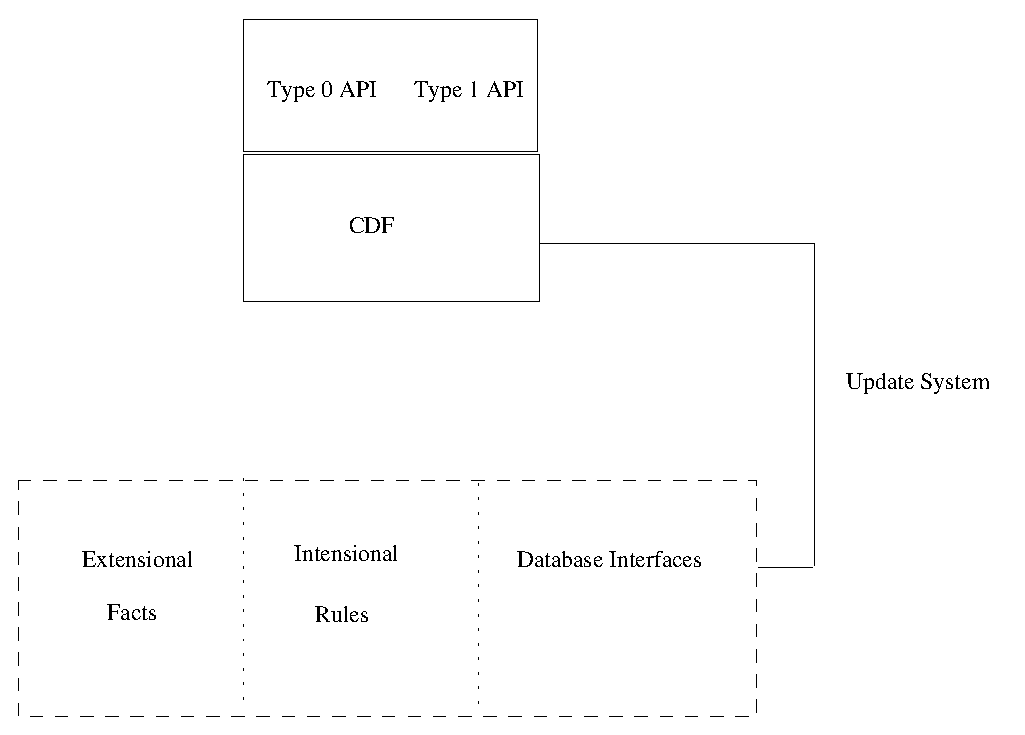
\epsfig{file=Figures/arch.eps,width=0.80\textwidth}}
\caption{A High-Level Architecture of CDF and XJ}
\label{fig:arch}
\end{figure}
%--------------

CDF instances can be classified either as Type-0 or a Type-1, each of
which has its own interface.  Type-0 instances are useful for storing
large amounts of information; and consistency and implication in
Type-0 instances is computable in polynomial time.  Type-0 instances
describe classes by existential and universal relations, qualified
number restrictions, and relational hierarchies, but descriptions omit
negation and disjunction. Type-0 instances also support a direct
product construction for objects and classes.  
\mycomment{
These product classes and objects can be useful for representing
certain types of non-binary relations, and are particularly useful for
incorporating knowledge represented as RDF facts \cite{}.  }
Information in Type-0 CDF instances is tightly coupled to XSB's
query mechanism, and CDF ensures that only the most specific answers
(according to a given inheritance hierarchy) are returned for any
Type-0 query.

Type-1 instances extend Type-0 instances to describe classes using
negation and disjunction, and thus permit descriptions that are
equivalent to an expressive description logic.  In fact, a Type-1 CDF
instance can be seen as a knowledge base in which various classes are
described via {\em class expressions}, which correspond to formulas in
description logics.  Reasoning in Type-1 instances is done via the CDF
theorem-prover.  Using the Type-1 API, users may ask whether a given
class or object is consistent, whether a given class expression is
consistent with a class or object; or whether a given class expression
is entailed by a given class or object.  The problems of determining
consistency or entailment of a Type-1 class expression have a high
degree of complexity.  To solve these problems the CDF theorem prover
uses several heuristics, but a determined (or unlucky) user can always
find class expressions that require a large amount of time to check.

Of course, ontology management systems require many features in
addition to reasoning and representation features \cite{MGPS03}.  We
mention some of these features.

\begin{itemize}
\item {\em A Semantic Checking System}.  CDF has various mechanisms for
ensuring consistency of objects and classes both at the Type-0 or
Type-1 level.  Various levels of consistency can be checked during
various operations on the CDF instance.
%
\item {\em A Component System}. Reusability of ontologies is supported
by the {\em component} structure of CDF.  An ontology component may be
maintained by separate users or organizations in different locations
and assembled in various ways by applications.
%
\item {\em A Concurrency System}. (Non open-source) Based on the
component structure, the {\em concurrency} mechanism for CDF allows
users to update their own CDF instances and to periodically update a
common store. Naturally, the various mechanisms in CDF for ensuring
consistency that are vital to ensuring coherency when users update
their systems concurrently.
%
\item {\em Database Interfaces}. (Non open-souce) CDF supports various
interfaces to databases so that CDF facts can be stored in a database
or mapped to database tables.
\end{itemize}

Based on these features, CDF can support user interfaces in a number
of ways.  One of the most convenient is to use a XSB/Java interface
such as InterProlog~\cite{Cale01} or JAXSB~(see
\texttt{http://xsb.sourceforge.net}) and then write a user interface in
Swing or some other Java Graphics library.  One of the easiest ways to
do this is to make use of the {\em XJ system} which allows Swing Gui
objects to be represented as Prolog terms (the XJ system is non
open-source) From a systems perspective, a graphical interface is then
written XJ library Swing widgets or specialized XJ-CDF Swing widgets.
CDF per-se has the following graphical packages and applications.
%
\begin{itemize}
%
\item {\em An XJ Caching System}. Adds and deletes to CDF are extended
with a notification mechanism so that Java Swing objects (created with
XJ, XSB's graphics system) reflect the state of CDF even when it
dynamically changes.
%
\item {\em A Visual Editor}. Finally,  CDF supports a graphical editor
that allows users both to visualize an ontology and to perform the
functions mentioned so far.
\end{itemize}
%
Extensional facts, intensional rules, updates, the Type-0 and Type-1
interfaces, consistency checking predicates and the full component
system are available as an open-source package for XSB.  Other
features, concurrency mechanisms, specialized database interfaces, XJ
support and the editor are not open-source.  The open-source code can
be obtained via \texttt{xsb.sourceforge.net}.  Inquiries about the full
Coherent Description System should be made to
\texttt{ode@xsb.com}.





%------------------------------------------------------------------------------
\part{A (somewhat) Formal Introduction to CDF} \label{part:semantics}

\chapter{The Meaning of Type-0 CDF Instances}
\label{chap:type0} 

%-------------------------------------------------------------------------------
\mycomment{
\subsection{Terminology}

In this paper we use standard logic programming terminology and
notation (e.g. \cite{Lloy84}), extended with the well-founded
semantics~\cite{VGR99}. In addition, we commonly make use of notation
for sentences and formulas in first-order logic.  While most of this
notation is readily apparent, we sometimes write a first-order formula
$\phi$ as $\phi[\overline{X}]$, where $\overline{X}$ is a {\em
superset} of the free variables in $\phi$.
}
%-------------------------------------------------------------------------------

Facts in both Type-0 and Type-1 CDF instances are closely related to
class expressions in description logics.  However, because CDF often
stores class expressions as Prolog facts in an unconventional way, and
because description logics may not be familiar to a logic programming
audience, we present here a somewhat formal introduction to how CDF
represents knowledge.  Users without a mathematical background can
ignore the various axioms and formal definitions that are presented in
this chapter.  Our approach is to introduce a semantics of CDF based
on a translation of a {\em CDF instance} into a set of first-order
logic sentences that constitute an {\em Ontology Theory} whose models
are the models of a CDF instance.  For simplicity of presentation the
description of CDF instances in this section omits certain details
about components, extensional facts and intenstional rules, and other
topics that will be introduced in later chapters.

We illustrate aspects of CDF by means of an example drawn from
electronic commerce.  Health care organizations, such as hospitals,
clinics, etc., have difficulties in buying disposable medical devices
such as sutures, bandages, gloves, and so on.  The difficulty arises
from the fact that these devices may be quite specialized, for intance
when they are used in surgery.  At the same time, since these devices
are disposable, they may need to be purchased frequently.  We consider
concretly the class of {\em absorbable sutures}, which are used for
stitching and securing tissues, and which can be absorbed by the human
body.  Information below is adapted from he U.S. Defence Logistics
Information Service \url{http://www.dlis.mil}, from the Universal
Standard Products and Services Classification~\cite{UNSPSC}, as well
as from websites of various commercial medical supply companies.

\section{Type-0 CDF Instances}
\label{sec:type0} 

We begin with the syntax of Type-0 instances~\footnote{The syntax for
identfiers differs in the actual CDF implementation. See
Section~\ref{sec:instance}.}: 

\begin{definition}[Type-0 Instances: Semantic Level] \label{def:ids}
A {\em Type-0 CDF instance} is a finite set of ground facts for the
predicates \pred{isa/2}, \pred{hasAttr/3}, \pred{allAttr/3},
\pred{classHasAttr/3}, \pred{minAttr/4}, and \pred{maxAttr/4}.  An {\em
identifier} is either a constant or a term.  The arguments of these
predicates are {\em concrete identifiers}, where a term $T$ is an
identifier iff $T$ has the functor symbol {\tt cid/1}, {\tt oid/1},
{\tt rid/1}, or {\tt crid/1} whose argument is either

\begin{enumerate}
\item a constant; or 
\item a term $f(I_1,\ldots,I_n)$ where $I_1,\ldots,I_n$ are identifiers.
\end{enumerate}
In the first case, an identifier is called {\em atomic}; in the second
it is called a {\em product identifier}.
\end{definition}

Despite the simple syntax of Type-0 CDF instances, their semantics
differs from the usual semantics assigned to facts in Prolog.
Identifiers identify sets of objects, or binary relations between
objects.  Furthermore, the facts of a Type-0 CDF instance can
implicitly denote inheritance of various relationships among classes
and objects, as well as inheritance constraints about what
relationships are allowed.

\subsection{Simple Taxonomies in CDF}

\begin{example} \rm \label{ex:suture1}
The following CDF instance illustrates a fragment of a taxonomy for
medical equipment.
%-------------------------------------------
{\tt  {\small 
\begin{tabbing}
foo\=foo\=foo\=foo\=foo\=foo\=foooo\=foooooooooooooooo\=\kill
isa(cid(medicalEquipment),cid('CDF Classes'))  \\
\> isa(cid(woundCareProducts),cid(medicalEquipment)) \\
\> \> \>  isa(cid(suturesAndRelatedProducts),cid(woundCareProducts)) \\
\> \> \> isa(cid(sutures),cid(suturesAndRelatedProducts))  \\
\> \> \> \> isa(cid(absorbableSutures),cid(sutures))  \\
\> \> \> \> isa(cid(nonAbsorbableSutures),cid(sutures)) \\
\> \\
\> \> \>   isa(oid(sutureU245H),cid(absorbableSutures))  \\
\> \> \> \> \>   isa(oid(suture547466),cid(sutures)) 
\end{tabbing} }} 
%-------------------------------------------
\noindent
In CDF, sets of objects are termed {\em classes} to stress the
informality of its sets from the perspective of set theory, and class
identifiers have the functor {\tt cid/1}.  One can read the fact
\begin{verbatim}
      isa(cid(nonAbsorbableSutures),cid(sutures))
\end{verbatim}
as ``all elements in the class {\tt cid(nonAbsorbableSutures)} are
also in the class {\tt cid(sutures)}'' --- in other words, that {\tt
cid(nonAbsorbableSutures)} is a subclass of {\tt cid(sutures)}.
Object identifiers have the functor {\tt oid/1}, and denote classes
with cardinality 1, or {\em singleton classes}.  The fact
\begin{verbatim}
      isa(oid(sutureU245H),cid(absorbableSutures))
\end{verbatim}
can be read as ``the element of the singleton class {\tt
oid(sutureU245H)} is in the class {\tt cid(absorbableSutures)}''.
Note that {\tt cid(absorbableSutures)} is (potentially) more specific
than the class {\tt cid(sutures)}, to which {\tt oid(suture547466)}
belongs.  The class {\tt cid('CDF Classes')} is taken to contain all
objects in the domain of discourse.  All identifiers in this simple
taxonomy are atomic.

The decision of whether to denote an entity as an object or as a class
depends on the use of a given CDF instance.  Here, a given part number
can specify a number of physical parts, but the physical parts are
taken to be identical for the purposes of this instance.  However, if
we were constructing a CDF instance for warehouse management, the
above objects might be better represented as classes, and the physical
objects represented as CDF objects.
\end{example} 

Implicit in the above example is the fact that we use the term {\em
object identifiers} or {\em objects} to denote singleton classes,
class identifiers to denote all classes (including singleton classes).
Elements cannot be denoted directly by CDF facts, but only through
singleton classes that contain them (and are isomorphic to them).  At
this point, we can begin defining the semantics of Type-0 CDF
instances.

%-------------------
\begin{definition} \label{def:ontolang}
\index{ontology language} \index{ontology structure} \index{ontology
theory}
%
An {\em ontology language} is a first-order language with equality
containing the predicates: {\em isClass/1, isElt/1, isRel/1, isCrel/1,
elt/2, rel/3, and crel/3}, and a countable set of constants.  An {\em
ontology structure} is a structure defined over an ontology language.
An {\em ontology theory} is a set of first-order sentences formed over
an ontology language that includes a set of {\em core axioms}, defined
below, along with the defined predicate:
\[
isObj(X) =_{def} isClass(X) \wedge 
	((elt(E_1,X) \wedge elt(E_2,X)) \Rightarrow E_1 = E_2)
\]
If $\cT$ is an ontology theory formed over an ontology
language $\cL$, an ontology structure $S$ over $\cL$ is a model of
$\cT$ if every sentence of $\cT$ is satisfied in $S$.
\end{definition}
%-------------------

\index{sorting predicates}
By convention we assume that the variables in an ontology language are
indexed by the set of natural numbers.  In this paper we will restrict
our attention to ontology languages whose constant and function
symbols are identifiers as described in Definition~\ref{def:ids}.
Informally $isClass/1$ indicates that an identifier $I$ is a class
name or {\em class identifier}; $isElt/1$ indicates that an identifier
$I$ is an element of a class; $isRel/1$ that $I$ is a {\em relation
identifier}; and $isCrel/1$ that $I$ is a {\em class-relation
identifier}; and $isObj/1$ that $I$ is an {\em object identifier}.  We
sometimes call these 5 predicates {\em sorting predicates}.
$elt(E,C)$ indicates that an element $O$ is a member of class
identifier $C$; $rel(O_1,R,O_2)$ indicates that an element $E_1$ has a
$R$ relation to an element $E_2$; and $crel(C_1,R,E)$ indicates that
the class identifier $C_1$ has a $R$ relation to an object identifier
$E$.

The first core axiom ensures that objects, classes, relations and
class-relations all have distinct identifiers within an ontology
language.
%-----------
\begin{axiom}[Distinct Identifiers] \label{ax:distinct}
\index{axioms!distinct identifiers} 
\ \\
\begin{tabbing}
foo\=foo\=foo\=foo\=foo\=foo\=foooo\=foooooooooooooooo\=\kill
\> $\neg \exists Id [isClass(Id) \wedge (isElt(Id) \vee isRel(Id) 
	                                 \vee isCrel(Id))] \wedge $ \\
\> $\neg \exists Id [isObj(Id) \wedge (isElt(Id) \vee isCrel(Id))] \wedge $ \\
\> $\neg \exists Id [isElt(Id) \wedge isCrel(Id)] $ 
\end{tabbing}
\end{axiom} 
%-----------

$isClass/1$, $isElt/1$, $isRel/1$, and $isCrel/1$ provide an effective
sorting that extends to all predicates, as the next axiom indicates.

\begin{axiom}[Predicate Sorts] \rm \label{ax:sorts}
\index{axioms!predicate sorts} 
\ \\
\begin{tabbing}
foo\=foo\=foo\=foo\=foo\=foo\=foooo\=foooooooooooooooo\=\kill
\> \> $(\forall X,Y) [elt(X,Y) \Rightarrow (isElt(X) \wedge isClass(Y))]
								\wedge $ \\
\> \> $(\forall X,Y,Z) [rel(X,Y,Z) \Rightarrow (isElt(X) \wedge isRel(Y)
					   \wedge isElt(Z))] \wedge  $ \\
\> \> $(\forall X,Y,Z) [crel(X,Y,Z) \Rightarrow (isClass(X) \wedge isRel(Y)
					   \wedge isElt(Z))] $ \\
\end{tabbing}
\end{axiom} 

%-----------

The following definition of $IdSort$ relates the functors of
identifiers in a Type-0 CDF instance to their sort in an ontology
theory.  It will be used in the various instance axioms to enforce
proper sorting of product identifiers.

\begin{definition}{\bf [IdSort]} \label{def:IdSort}
Let {\em I} is be an identifier. Then {\em IdSort(I)} is equal to {\em
isClass(I)} if the main functor symbol of {\em I} is {\tt cid/1}; {\em
isObj(I)} if the main functor symbol of {\em I} is {\tt oid/1}; {\em
isRel(I)} if the main functor symbol of {\em I} is {\tt rid/1}; and
{\em isCrel(I)} if the main functor symbol of {\em I} is {\tt crid/1}.
\end{definition}

%-----------------------------------------------------------------------------------------
\mycomment{
\begin{definition}{\bf [IdSort]}  Let {\em I} is be an identifier, and
$\cI$ be the set of identifiers occurring in {\em I}. Then
%
\[ IdSort(I) =_{def} \bigwedge_{I' \in \cI} Sort(I') \]
%
where {\em Sort(I)} is equal to {\em isClass(I)} if the main functor
symbol of {\em I} is {\tt cid/1}; {\em isObj(I)} if the main functor
symbol of {\em I} is {\tt oid/1}; {\em isRel(I)} if the main functor
symbol of {\em I} is {\tt rid/1}; and {\em isCrel(I)} if the main
functor symbol of {\em I} is {\tt crid/1}.
\end{definition}
}
%-----------------------------------------------------------------------------------------

From Definitions~\ref{def:IdSort} and~\ref{def:ontolang}, it is easy
to see that for any object identifier $O$, $IdSort(O) = isObj(O)$, and
$isObj(O) \Rightarrow isClass(O)$.

%-----------
\begin{instance} [Translation of {\tt isa/2}] \rm 
For each fact of the form {\tt isa(Id$_1$,Id$_2$)} add the axiom
\ \\
\begin{tabbing}
foo\=foo\=foo\=foo\=foo\=foo\=foooo\=foooooooooooooooo\=\kill
\> $ IdSort(Id_1) \wedge IdSort(Id_2) \wedge $ \\

\> \> $ (((isClass(Id_1) \wedge isClass(Id_2)) \wedge
	(\forall X) [elt(X,Id_1) \Rightarrow elt(X,Id_2)]) \vee $ \\

%\> \> $ ((isObj(Id_1) \wedge isClass(Id_2)) \wedge elt(Id_1,Id_2)) \vee $ \\

\> \> $ ((isRel(Id_1) \wedge isRel(Id_2)) \wedge
	(\forall X,Y)[rel(X,Id_1,Y) \Rightarrow rel(X,Id_2,Y)]) \vee $ \\

\> \> $ ((isCrel(Id_1) \wedge isCrel(Id_2)) \wedge
	(\forall X,Y)[crel(X,Id_1,Y) \Rightarrow crel(X,Id_2,Y)])) $ 
\end{tabbing}
denoted as {\tt isa(Id$_1$,Id$_2$)}$^{\cI}$.
\end{instance}
%-----------

Note that the reflexive and transitive closure of {\tt isa/2} is an
immediate consequence of its translation rule.  The next axiom is
technical.  It is important for the semantics of relations that each
class have at least one member.
%-----------
\begin{axiom}[Non-Empty Classes] \label{ax:nonnull}
\index{axioms!non-empty classes} 
\[ (\forall X) [isClass(X) \Rightarrow (\exists Y) [elt(Y,X)]] \]
\end{axiom} 
%-----------

The last core axiom for these predicates ensures is that each class is
a subclass of {\tt cid('CDF Classes')}.

%-----------
\begin{axiom}[Domain Containment] \label{ax:contained}
\index{axioms!domain containment} 
\[ (\forall X) [isElt(X) \Rightarrow elt(X,cid('CDF\ Classes'))] \]
\end{axiom} 
%-----------

\subsection{General Relations between Objects in  Classes}

\begin{example} \rm \label{ex:suture2}
The class {\tt cid(sutures)} can be further defined by its relations
to other classes.  For instance, an object in {\tt cid(sutures)} may
have a designation of its needle design indicating whether it is to be
used for abdominal surgeries, thoracic surgeries, or other purposes.
This information is indicated by the following CDF facts:
%
{\small
\begin{tabbing}
fooo\=foo\=foo\=foo\=fooooooooooooooooooooooooooooooo\=ooooooooooooo\=\kill
\> {\tt isa(rid(hasNeedleDesign),rid('CDF Relations'))} \\
\\
\> {\tt isa(cid(domainTypes),cid('CDF Classes'))} \\
\> \> {\tt isa(cid(needleDesignTypes),cid(domainTypes))} \\
\> \> \> {\tt isa(cid(Abdominal),cid(needleDesign))} \\
\> \> \> {\tt isa(cid(Abscisson),cid(needleDesign))} \\
\> \> \> {\tt isa(cid('Adson Dura'),cid(needleDesign))} \\
\> {\it \% 126 other values..}  \\
\\
\> {\tt allAttr(cid(sutures),rid(hasNeedleDesign),cid(needleDesign))} 
\end{tabbing}
}
%
\noindent
The {\tt allAttr/3} fact above can be read as ``if any object in {\tt
cid(absorbableSutures)} has a {\tt rid(hasNeedleDesign)} relation, it
must be to an object in the class {\tt cid(needleDesign)}''.  That
{\tt hasNeedleDesign} is a relation is indicated by clothing it in the
functor {\tt rid/1}.  This relation is an immediate subclass of all
{\tt CDF Relations} which in turn is taken to represent the universal
binary relation over the domain of discourse.  Thus the {\tt
allAttr/3} fact effectively types the range of {\tt
rid(hasNeedleDesign)} relations, stemming from objects in the class
{\tt cid(absorbableSutures)}, but it does not indicate the existence
of such a relationship.  From a user's point of view, the {\tt
rid(hasNeedleDesign)} relation can be thought of as an optional
attribute for a given {\tt cid(absorbableSutures)} object.  Sample
values for {\tt cid(hasNeedleDesignTypes)} are also given.
\end{example} 

%-------------------

{\tt allAttr/3} provides a simple but powerful mechanism for
inheritance of typing among CDF classes:
%---------------------------------------------------------------------------
\mycomment{
, as can be seen from the
following translation rule, which uses the defined formula

\[ 
elt(X,Y) =_{def} ((isClass(Y) \wedge elt(X,Y)) \vee (isObj(Y) 
			\wedge X = Y))
\] }
%---------------------------------------------------------------------------

\begin{instance} [Translation of {\tt allAttr/3}] \rm 
For each fact of the form {\tt allAttr(Id$_1$,Rid,Id$_2$)} add the instance
axiom: 
\begin{tabbing}
foo\=foo\=foo\=foo\=foo\=foo\=foooo\=foooooooooooooooo\=\kill
\> $ IdSort(Id_1) \wedge IdSort(Rid) \wedge IdSort(Id_2) \wedge $ \\
\> \> $ IsClass(Id_1) \wedge IsRel(Rid) \wedge IsClass(Id_2) \wedge $ \\
\> \> $(\forall X, Y) [(elt(X,Id_1) \wedge rel(X,Rid,Y))
					\Rightarrow elt(Y,Id_2)] $
\end{tabbing}
denoted as {\tt allAttr(Id$_1$,Rid,Id$_2$)$^{\cI}$}.
\end{instance}

%----------------------
\mycomment{
\begin{tabbing}
foo\=foo\=foo\=foo\=foo\=foo\=foooo\=foooooooooooooooo\=\kill
\> $ IdSort(Id_1) \wedge IdSort(Rid) \wedge IdSort(Id_2) \wedge $ \\
\> \> $ (IsClass(Id_1) \vee isObj(Id_1)) \wedge IsRel(Rid) \wedge 
	 (IsClass(Id_2) \vee isObj(Id_2)) \wedge $ \\
\> \> $(\forall X, Y) [(elt(X,Id_1) \wedge rel(X,Rid,Y))
					\Rightarrow elt(Y,Id_2)] $
\end{tabbing}
}
%----------------------
\begin{example} \rm \label{ex:hasAttr}
While {\tt allAttr/3} indicates a typing for relations, it does not
indicate that a relation must exist for elements of a class.  This
statement is made by \pred{hasAttr/3}.  The relation {\tt
rid(hasPointStyle)} for the class {\tt cid(absorbableSutures)} is
taken to be required in this schema.  The facts
%
{\small
\begin{tabbing}
fooo\=foo\=foo\=foo\=foooooooooooooooooooooooooooo\=ooooooooooooo\=\kill
\> {\tt allAttr(cid(absorbableSutures),rid(hasPointStyle),cid(pointStyle)) } \\
\> {\tt hasAttr(cid(absorbableSutures),rid(hasPointStyle),cid(pointStyle)) }
\end{tabbing}
}
%
\noindent
indicate not only the range of such relationships, but that such a
relationship must exist.  Indeed, the {\tt hasAttr/3} fact can be read
as ``all objects in the class {\tt cid(absorbableSutures)} have a
relation {\tt rid(hasPointStyle)} to an object in the class {\tt
cid(pointStyle)}''.  The facts below also give information about the
{\tt rid(hasPointStyle)} relation.
%
{\small
\begin{tabbing}
fooo\=foo\=foo\=foo\=foooooooooooboooooooooooooooo\=ooooooooooooo\=\kill
\> {\tt isa(cid(pointStyle),cid(domainTypes))} \\
\> {\tt isa(cid(regularCuttingEdge),cid(pointStyle))} \\
\> {\tt isa(cid(reverseCuttingEdge),cid(pointStyle))} \\
\> {\tt isa(cid(scalpelPoint),cid(pointStyle))} \\
\> {\it \% 10 other values.} \\
\\
\> {\tt hasAttr(oid(sutureU245H),rid(hasPointStyle),cid(regularCuttingEdge))}
\end{tabbing}
} 
\noindent
The last of the above facts can be read as ``the object {\tt
oid(sutureU245H)} has a {\tt rid(hasPointStyle)} relation to an object
in the class {\tt cid(pointStyle)}''.  
\end{example}

Not surprisingly, the definition of {\tt hasAttr/3} bears some
similarity to that of {\tt allAttr/3}.

\begin{instance} [Translation of \pred{hasAttr/3}] \rm 
For each fact of the form {\tt hasAttr(Id$_1$,Rid,Id$_2$)} add the instance
axiom: 
\begin{tabbing}
foo\=foo\=foo\=foo\=foo\=foo\=foooo\=foooooooooooooooo\=\kill
\> $ IdSort(Id_1) \wedge IdSort(Id_2) \wedge IdSort(Id_2) \wedge $ \\
\> \> $ IsClass(Id_1) \wedge IsRel(Rid) \wedge
	 IsClass(Id_2) \wedge $ \\
\> \> \> $ (\forall X) [elt(X,Id_1) \Rightarrow \exists Y [rel(X,Rid,Y) 
					\wedge elt(Y,Id_2)]]$
\end{tabbing}
denoted as {\tt hasAttr(Id$_1$,Rid,Id$_2$)$^{\cI}$}.
\end{instance}

We next turn to relational axioms that indicate the cardinality of
various relations.

\begin{example} \rm  \label{ex:maxAttr}
For our purposes, an object in {\tt cid(absorbableSutures)} can be
thought of as consisting of a needle and a thread~\footnote{The thread
is often called a suture.  We are assuming for purposes of
illustration that all sutures are --- in suture-speak --- ``armed''.}.  This is
represented by the facts:
%
{\small
\begin{tabbing}
foo\=foo\=foo\=foo\=foo\=foo\=foooo\=foooooooooooooooo\=\kill
\> {\tt allAttr(cid(absorbableSutures),rid(hasImmedPart),cid(absSutPart)) } \\
\> {\tt hasAttr(cid(absorbableSutures),rid(hasImmedPart),cid(absSutNeedle)) } \\
\> {\tt hasAttr(cid(absorbableSutures),rid(hasImmedPart),cid(absSutThread)) } \\
\\
\> {\tt isa(cid(absSutPart),cid(suturesAndRelatedProducts))}  \\
\> \> {\tt isa(cid(absSutNeedle),cid(absSutPart)) } \\
\> \> {\tt isa(cid(absSutSuture),cid(absSutPart)) } 
\end{tabbing}
}
%
\noindent
A needle for an absorbable suture is typically made of a different
material than the thread to which the needle is attached.  Each of
these materials may be important in choosing an absorbable suture, and
each of these materials are unique.  The facts
%
{\small
\begin{tabbing}
foo\=foo\=foo\=foo\=foo\=foo\=foooo\=foooooooooooooooo\=\kill
\> {\tt hasAttr(cid(absSutPart),rid(hasMaterial),cid(absSutMaterial)) } \\
\> {\tt maxAttr(cid(absSutPart),rid(hasMaterial),cid(absSutMaterial),1) } \\
\\
\> {\tt isa(cid(material),cid(domainTypes))} \\
\> {\tt isa(cid(absSutMaterial),cid(material)} \\
\> {\tt isa(cid(gut),cid(absSutMaterial))} \\
\> {\tt isa(cid(polyglyconate),cid(absSutMaterial))} \\
\> {\tt isa(cid(polyglyconicAcid),cid(absSutMaterial)) } 
\end{tabbing}
}
%
\noindent
indicate that each {\tt cid(absSutPart)} has a unique material.  The
{\tt maxAttr/4} fact can be read as ``Each object in the class {\tt
cid(absSutPart)} has at most 1 {\tt rid(hasMaterial)} relation to an
object in the class {\tt cid(absSutMaterial)}''.
\end{example}

In order to define the semantics of {\tt maxAttr/4}, let
$\exists^{\leq n}X_m[ \phi(X,Z)]$ be defined as an abbreviation for
the formula
\[
  \exists x_m,...,\exists x_{m+n} [\bigwedge_{m \leq i \leq m+n} 
	\phi(x_i,\overline{z}) 
	\Rightarrow \bigvee_{m \leq i < j \leq m+n} x_i  = x_j]
\]
i.e., for the formula indicating that there are at most $N$ non-equal
elements satisfying $\phi(x,z)$.  The abbreviation $\exists^{\geq N}$
is defined similarly to indicate that a formula is satisfied by at
least $N$ non-equal elements.

\begin{instance} [Translation of {\tt maxAttr/4}] \rm 
For each fact of the form {\tt maxAttr(Id$_1$,Rid,Id$_2$,N)} add the instance
axiom: 
\begin{tabbing}
foo\=foo\=foo\=foo\=foo\=foo\=foooo\=foooooooooooooooo\=\kill
\> $ IdSort(Id_1) \wedge IdSort(Id_2) \wedge IdSort(Id_2) \wedge $ \\
\> \> $ IsClass(Id_1) \wedge IsRel(Rid) \wedge
	 (IsClass(Id_2) \wedge $ \\
\> \> \> $ (\forall X) [elt(X,Id_1) \Rightarrow \exists^{\leq N} Y [rel(X,Rid,Y) 
					\wedge elt(Y,Id_2)]]$
\end{tabbing}
denoted as {\tt maxAttr(Id$_1$,Rid,Id$_2$,N)$^{\cI}$}.
\end{instance}

A corresponding predicate, {\tt minAttr/4} is used to indicate a
minimality restriction on a relation.  {\tt minAttr/4} is defined
similarly to {\tt maxAttr/4}, but using $\exists^{\geq N}$ rather than
$\exists^{\leq N}$.  Indeed, the predicate
%
{\small {\tt 
\begin{tabbing}
foo\=foo\=foo\=foo\=foo\=foo\=foooo\=foooooooooooooooo\=\kill
\> hasAttr(cid(absSutPart),rid(hasMaterial),cid(absSutMaterial)).
\end{tabbing}
} }
%
\noindent
could be replaced by the predicate
%
{\small {\tt 
\begin{tabbing}
foo\=foo\=foo\=foo\=foo\=foo\=foooo\=foooooooooooooooo\=\kill
\> minAttr(cid(absSutPart),rid(hasMaterial),cid(absSutMaterial),1).
\end{tabbing}
} }
%
\subsection{Class Relations}
Each of the predicates discussed so far are inheritable in their first
argument.  For instance, the fact
{\small {\tt 
\begin{tabbing}
foo\=foo\=foo\=foo\=foo\=foo\=foooo\=foooooooooooooooo\=\kill
\> hasAttr(cid(absSutPart),rid(hasMaterial),cid(absSutMaterial)).
\end{tabbing}
} } 
%
\noindent
implies that every subclass of {\tt cid(absSutures)} will have a
material in the class {\tt cid(absSutMaterial)}.  However, classes may
have relations that do {\em not} hold for their subclasses or members.
For instance, a finite set may have a given cardinality, but its
proper subsets will have a different cardinality.  Such relations are
termed {\em class relations}.

%-------------------
\begin{example} \label{ex:strel} \rm 
A practical example of a class relation comes from an application that
may be called part equivalency matching.  In this application, the
possible attributes for a class of parts are given various weights.
Two parts match if the sum of the weights of their attributes that
match are above a given threshold.  The weighting for the {\tt
cid(pointStyle)} of sutures might be given as:
%----------------------------------
{\small 
{\tt 
\begin{tabbing}
foo\=foo\=foo\=foo\=foo\=foo\=foooo\=foooooooooooooooo\=\kill
\> isa(cid(pointStyleWeight),cid('CDF Classes')) \\
\> \> isa(cid(highWeight),cid(pointStyleWeight)) \\
\> \> isa(cid(lowWeight),cid(pointStyleWeight)) \\
\\
\> classHasAttr(cid(sutures),crid(pointStyleWeight),cid(highWeight))
\end{tabbing}
} }
%----------------------------------
\noindent
The {\tt classHasAttr/3} fact can be read as ``the class {\tt
cid(sutures)} has a {\tt crid(pointStyleWeight)} relation to an object
in {\tt cid(highWeight)}.  Matching weights are made non-inheritable
via {\tt classHasAttr/3} because a weight may depend on a given
classification of a part.  For instance if a part were classified as a
{\tt cid(nonAbsorbableSuture)}, its {\tt cid(pointStyle)} might weigh
less (or more) for determining whether two sutures are equivalent.
\end{example}
%------------------
\begin{instance} [Translation of {\tt classHasAttr/3}] \rm 
For each fact of the form {\tt classHasAttr(Id$_1$,CRid,Id$_2$)} add the
instance axiom: 
\begin{tabbing}
foo\=foo\=foo\=foo\=foo\=foo\=foooo\=foooooooooooooooo\=\kill
\> $ IdSort(Id_1) \wedge IdSort(CRid) \wedge IdSort(Id_2) \wedge $ \\
\> \> $ IsClass(Id_1) \wedge IsCrel(CRid) \wedge isClass(Id_2) \wedge $ \\
\> \> \> $ (\exists X) [elt(X,Id_2) \wedge crel(Id_1,CRid,X)] $
\end{tabbing}
denoted as {\tt classHasAttr(Id$_1$,Rid,Id$_2$)$^{\cI}$}.
\end{instance}
%----------


  \section{Product Classes}

The above predicates allow the definition of various named binary
relations between classes.  However, binary definitions can sometimes
be inconvenient to use.  For instance, in the part equivalency
matching example, (Example~\ref{ex:strel}), it may be desirable to
make explicit the weight of the match as an indication of the strength
of the match.  The weight could be made explicit by a series of
definitions
%-------------------------------------------
{\small 
{\tt 
\begin{tabbing}
foo\=foo\=foo\=foo\=foo\=foo\=foooo\=foooooooooooooooo\=\kill
\> allAttr(\cid{dlaPart},\rid{suturesRusMatch\_low},\cid{suturesRusPart}) \\
\> : \\
\> allAttr(\cid{dlaPart},\rid{suturesRusMatch\_high},\cid{suturesRusPart})
\end{tabbing}
} } 
%----------------------------------
\noindent
indicting that a given part has a match of weight {\em low} through
{\em high}.  However, for a scale with a large number of values,
defining matches in this way is time-consuming and prone to errors.
To address this, we first define a new class {\tt \cid{matchScale}}
containing as subclasses the various match levels.  We then combine
{\tt \cid{matchScale}} with the class {\tt \cid{suturesRusPart}} in a
product with a {\em product identifier}, as in the following fact
%-------------------------------------------
{\small 
{\tt 
\begin{tabbing}
foo\=foo\=foo\=foo\=foo\=foo\=foooo\=foooooooooooooooo\=\kill
 
allAttr(\cid{dlaPart},\rid{suturesRusMatch}, \\
\> \> \> \> \cid{partMach(\cid{suturesRusPart},\cid{matchScale})})
\end{tabbing}  } }
\noindent 
which indicates that a {\tt \cid{dlaPart}} can have a {\tt
\cid{suturesRusMatch}} to an object in the {\tt partMatch/2}  class,
which has both a {\tt \cid{suturesRusPart}} component and a {\tt
\cid{matchScale}} component.

%-------------------------------------------------------------------

We capture the intuition behind product classes through the following
axiom schemas.  The first indicates that product identifiers 
are constructed from {\em constituent identifiers} of the same sort.

\begin{axiom}[Downward Closure] \label{ax:downcl}
\index{axioms!downward closure}
\ \\
For each product identifier $\cid{f(x_1,\ldots,x_n)}$,
$\oid{f((x_1,\ldots,x_n)}$, $\rid{f(x_1,\ldots,x_n)}$, and
$c\rid{f((x_1,\ldots,x_n)}$ the following axiom is added,
\begin{tabbing}
foo\=foo\=foo\=foo\=foo\=foo\=foooo\=foooooooooooooooo\=\kill
\> $isClass(\cid{f(x_1,\ldots,x_n)}) \Rightarrow 
	isClass(x_1) \wedge \ldots \wedge isClass(x_n) $\\
\> $isObj(\oid{f(x_1,\ldots,x_n)}) \Rightarrow 
	isObj(x_1) \wedge \ldots \wedge isObj(x_n) $\\
\> $isRel(\rid{f(x_1,\ldots,x_n)}) \Rightarrow 
	isRel(x_1) \wedge \ldots \wedge isRel(x_n) $\\
\> $isCrel(\crid{f(x_1,\ldots,x_n)}) \Rightarrow 
	isCrel(x_1) \wedge \ldots \wedge isCrel(x_n) $
\end{tabbing}
\end{axiom}

With this axiom, along with the use of $IdType/1$ in the various
instance axioms, we will sometimes refer to a CDF identifier $I$ as a
class identifier if its outer functor is {\tt cid/1}, an object
identifier if its outer functor is {\tt oid/1} etc.  The next axiom
associates product classes with the objects they contain.

\begin{axiom}[Implicit Subclassing] \label{ax:implsc}
\index{axioms!implicit subclassing} 

\begin{enumerate}
\item For each product identifier $cid(f(x_1,\ldots,x_n))$ or 
$oid(f(x_1,...,x_n))$, the following axioms are added for $x_i, 1 \leq i
\leq n$:
\[
(\forall E) [(elt(E,y_i) \Ra elt(E,x_i)) \Ra \\
	(\forall E') [elt(E',f(x_1,...x_n))[x_i/y_i] \Rightarrow elt(E',f(x_1,...x_n))]]
\]

\item For each product identifier $rid(f(x_1,\ldots,x_n))$ the
following axioms are added for $x_i, 1 \leq i 
\leq n$:
\begin{tabbing}
foo\=foo\=foo\=foo\=foo\=foo\=foooo\=foooooooooooooooo\=\kill
\> $(\forall E_1,E_2) [(rel(E_1,y_i,E_2) \Ra rel(E_1,x_i,E_2)) \Ra$ \\
\> \> $(\forall E'_1,E'_2) [rel(E'_1,f(x_1,...x_n),E'_2)[x_i/y_i] \Ra rel(E'_1,f(x_1,...x_n),E'_2)]]$
\end{tabbing}
\end{enumerate}
\end{axiom}

%-------------------------------------------
\mycomment{
\begin{axiom}[Implicit Subclassing] \label{ax:implsc}
\begin{enumerate}
\item For each product identifier $\oid{f(x_1,\ldots,x_n)}$ the
following axiom is added:  
\[(\forall O) [elt(O,\cid{f(x_1,\ldots,x_n)})
	\Ra (O = \oid{f(y_1,\ldots,y_n)} \wedge 
  		  elt(y_1,x_1) \wedge \ldots \wedge elt(y_n,x_n))] \]

\item For each product identifier $\cid{f(x_1,\ldots,x_n)}$ and for
each atomic identifier $\cid{c}$ the following axiom is
added:
\[ (\forall C) 
   ([elt(\oid{f(x_1,\ldots,x_n)},C)] \Ra (C = \cid{f(y_1,\ldots,y_n)}
   \vee C = \cid{c})) \]
\end{enumerate}
\end{axiom}
}
%-------------------------------------------

\begin{example} \rm
Axiom~\ref{ax:downcl} simply states that identifier types cannot be
mixed within a product identifier.  For instance, if {\tt
\oid{matchLevelN}} is an object in the {\tt \cid{matchScale}},
then the identifier 

{\tt \cid{partMatch(\cid{suturesRusMatch},\oid{matchLevelN})}}

\noindent
is improperly formed.  On the other hand, if {\tt \oid{sutureU245H}} is in
the class {\tt \cid{suturesRusPart}}, then the identifier {\tt
\oid{partMatch(\oid{sutureU245H},\oid{matchLevelN})}} is a product
identifier that is also an object identifier.

Axiom~\ref{ax:implsc} also means that the inheritance relation of a
product class is partly determined by the inheritance relation of its
constituent elements.
\end{example}

\mycomment{
Core Axiom~\ref{ax:implsc} can be used either to set up equality
constraints on a model of a CDF instance, or it can be used to
determine which CDF instances have free models (as explained in the
next section).  The following example illustrates the first use.

\begin{example} \rm \label{ex:equality}
Suppose we have the CDF instance
{\small 
{\tt 
\begin{tabbing}
foo\=foo\=foo\=foo\=foo\=foo\=foooo\=foooooooooooooooo\=\kill
\> isa(\cid{a},\cid{f(a)}.
\end{tabbing} } } 
\noindent
By Core Axiom~\ref{ax:nonnull} (Non-empty Classes), {\tt \cid{a}} has
at least one element, which can be called {\tt \oid{a1}}.  By the
instance axiom for the above fact, {\em elt(\oid{a1},\cid{f(a)}}.  By
Core Axiom~\ref{ax:implsc}(1), it must be the case that 
%
\[ \oid{a1} = \oid{f(Y)} \wedge elt(Y,\cid{a}) \]
%
If we take $Y = \oid{a1}$, then this means that 
%
$ \oid{a1} = \oid{f(\oid{a1})} $
% 
so that the above fragment has a model $\cM$ with a single individual
(in the universe of $\cM$) to which all object identifiers are mapped,
and that has a $elt/2$ relation to each individual to which a class
identifier is mapped (among other models).
\end{example}
}

\section{Models of Type-0 Instances} \label{sec:type0models}

Type-0 instances have been designed so that checking their consistency
--- whether they have a model --- is easily done.  Models of Type-0
instances are discussed in \cite{SwiW03b}, here we review some of the
main points without proofs.  We begin by defining a model of a Type-0
instance.

\begin{definition} \label{def:ont-th}
Let $\cO$ be a CDF instance.  We define as $\cL_{\cO}$, the ontology
language whose functions and constant symbols are restricted to the
identifiers in $\cO$.  $TH(\cO)$ is the ontology theory over
$\cL_{\cO}$ whose non-logical axioms consist of the core axioms and
the instance axiom for each fact in $\cO$.
% while $\cO^{\cI}$ is the theory over $\cL_{\cO}$ containing only the
% instance axioms.  
We say that an ontology structure $\cM$ is a model of $\cO$ if it is a
model of $TH(\cO)$.

\index{well-sorted}
If $\cO$ is Type-0 it is {\em well-sorted} if each instance axiom
cojoined with Core Axioms~\ref{ax:distinct} (Distinct Identifiers) and
Axiom Schema~\ref{ax:downcl} (Downward Closure) is consistent.
\end{definition}

Intuitively, a CDF fact is well-sorted if its arguments have class,
relation, class relation identifiers, etc. in the right place.  There
is no room for contradiction in a well-sorted Type-0 instance $\cO$
unless it contains {\tt minAttr/4} and {\tt maxAttr/4} facts.  If it
does, inconsistency can arise if {\tt minAttr(C$_1$,R,C$_2$,M)}$^{\cI}$
holds, {\tt maxAttr(C$_1$,R,C$_2$,N)}$^{\cI}$ holds, and $M > N$.
Thus, consistency of Type-0 instances is easy to check, and can in
fact be done in polynomial time.

However, CDF is a logic programming system, so it is important to know
whether an instance $\cO$ over a language $\cL_{\cO}$ has a {\em
Herbrand} model \cite{Lloy84} --- essentially one in which the
universe $\cU$ of the model are the terms of $\cL_{\cO}$, and where
the mapping of terms from $\cL_{\cO}$ to $\cU$ is the identity
mapping.  Herbrand models are the basis of Prolog semantics, so that
if CDF instances have Herbrand models, they can be easily implemented
in Prolog without resorting to a constraint system or to
meta-interpretation.  Care has been taken to ensure that any Type-0
CDF instance does in fact have a Herbrand model, so that the Type-0
interface in \refchap{sec:impl} can be supported~\footnote{This is one
of the reasons why object identifiers in CDF denote singleton classes.
If two classes $c_1$ and $c_2$ are ``equal'', this simply means that a
model must satisfy the sentence $(\forall X) elt(X,c_1)
\leftrightarrow elt(X,c_2)$ which has a Herbrand model.}.

  \section{Inheritance} \label{sec:inheritance}

Example~\ref{ex:hasAttr} indicates that each object in the class of
{\tt cid(absorbableSutures)} has a {\tt rid(hasPointStyle)} relation
to an object in the domain {\tt cid(pointStyle)}.  Thus, if no
stronger information were provided for, say, part {\tt
oid(sutureU245H)}, then
%--------------------------
{\small 
\begin{tabbing}
foo\=foo\=foo\=foo\=foo\=foo\=foooo\=foooooooooooooooo\=\kill
\> {\tt hasAttr(oid(sutureU245H),rid(hasPointStyle),cid(pointStyle))}$^{\cI}$
\end{tabbing} } 
%--------------------------
\noindent would be true in any model of the CDF instance.  This
consequence can be seen as a primitive form of ``default'', or more
precisely indefinite, reasoning that is provided by CDF.  Indeed,
%--------------------------
{\small 
\begin{tabbing}
foo\=foo\=foo\=foo\=foo\=foo\=foooo\=foooooooooooooooo\=\kill
\> {\tt
hasAttr(cid(suture547466),rid(hasPointStyle),cid(pointStyle))$^{\cI}$} 
\end{tabbing} } 
%--------------------------
\noindent would also be true, but would be of less interest, since
Example~\ref{ex:hasAttr} specifically indicates that {\tt
oid(suture547466)} is related to a subclass of {\tt cid(pointStyle)},
namely {\tt cid(regularCuttingEdge)}.  In contrast to {\tt
rid(endType)} the relation {\tt rid(suturesRusMatch)} was defined via
the {\tt allAttr/3} predicate.  
However the constraint that any {\tt rid(suturesRusMatch)} must be to
a {\tt cid(suturesRusPart)} holds for members of the class {\tt
cid(sutures)}, just as it holds for subclasses of {\tt
cid(sutures)}. 
The following formulas summarize inheritance in the
first argument of Type-0 relations.

%{\sc TLS: coversAttr}

\begin{proposition}[First Argument Inheritance Propagation] \label{prop:inh1}\rm
Let $\cM$ be an ontology model.
\begin{enumerate}
\item If $\cM \models {\tt hasAttr(Id_1,Id_2,Id_3)}^{\cI} \wedge
						{\tt isa(Id_0,Id_1)}^{\cI}$ 
	then $\cM \models  {\tt hasAttr(Id_0,Id_2,Id_3)}^{\cI}$
%
\item If $\cM \models {\tt allAttr(Id_1,Id_2,Id_3)}^{\cI} \wedge
					    {\tt isa(Id_0,Id_1)}^{\cI}$ 
		then $\cM \models {\tt allAttr(Id_0,Id_2,Id_3)}^{\cI}$ 
\item If $\cM \models {\tt minAttr(Id_1,Id_2,Id_3,N)}^{\cI} \wedge
						{\tt isa(Id_0,Id_1)}^{\cI}$ 
	then $\cM \models  {\tt minAttr(Id_0,Id_2,Id_3,N)}^{\cI}$
%
\item If $\cM \models {\tt maxAttr(Id_1,Id_2,Id_3,N)}^{\cI} \wedge
					    {\tt isa(Id_0,Id_1)}^{\cI}$ 
		then $\cM \models {\tt maxAttr(Id_0,Id_2,Id_3,N)}^{\cI}$ 
%
%\item If $\cM \models {\tt coversAttr(Id_1,Id_2,Id_3)}^{\cI} \wedge
%					    {\tt isa(Id_0,Id_1)}^{\cI}$ 
%		then $\cM \models {\tt coversAttr(Id_0,Id_2,Id_3)}^{\cI}$ 
%
\end{enumerate}
\end{proposition}



There is inheritance also in the third argument of relations.
Consider again the {\tt hasAttr/3} facts of Example~\ref{ex:hasAttr}
that states that any element of {\tt cid(absorbableSutures)} is
related via {\tt rid(hasPointStyle)} to an element or subclass of {\tt
cid(pointStyle)}.  By this definition, it also holds that {\tt
rid(hasPointStyle)} constrains any element of {\tt rid(absorbaleSutures)}
to an element or subclass of any {\em superclass} of {\tt
cid(pointStyle)} so that
%--------------------------
{\small 
\begin{tabbing}
foo\=foo\=foo\=foo\=foo\=foo\=foooo\=foooooooooooooooo\=\kill
\> 
{\tt hasAttr(cid(absorbableSutures),rid(hasPointStyle),cid('CDF Classes'))}$^{\cI}$
\end{tabbing} }
%--------------------------
\noindent
should also hold in any model of the CDF instance.  
%-----------------------
Similiarly,
{\small 
\begin{tabbing}
foo\=foo\=foo\=foo\=foo\=foo\=foooo\=foooooooooooooooo\=\kill
\> 
{\tt allAttr(cid(dlaPart),rid(suturesRusMatch),id('CDF Classes'))$^{\cI}$}
\end{tabbing} }
%-----------------------
\noindent
should also hold.  In English, every member or subclass of {\tt
cid(sutures)} that has a relation {\tt rid(suturesRusMatch)} has the
same relation to a member or subclass of {\tt \cid{'CDF Classes'}}.
{\tt minAttr/4} and {\tt classHasAttr/4} behave similarly with regards
to third argument inheritance.

Third argument inheritance is different for {\tt maxAttr/4}, however.
The fact
%-----------------------
{\small 
\begin{tabbing}
foo\=foo\=foo\=foo\=foo\=foo\=foooo\=foooooooooooooooo\=\kill
\> 
{\tt maxAttr(cid(person),rid(hasGeneticRelation),cid(mother))}
\end{tabbing} }
%-----------------------
\noindent
states that each person has at most one genetic mother.  If {\tt
cid(mother)} is a subclass of {\tt cid(parent)}, then it is not true
that each person has at most one genetic parent.  On the other hand,
if {\tt cid(elderlyMother)} is a subclass of {\tt cid(mother)} then it
is true that each person has at most one genetic elderly mother.  The
behavior of {\tt maxAttr/4} in models of CDF instances accords with
this intuition.
%-----------------------

\begin{proposition}[Third-Argument Inheritance Propagation] \rm
\label{prop:inh3} 
\end{proposition} 
\begin{enumerate}
\item If $\cM \models {\tt hasAttr(Id_1,Id_2,Id_3)}^{\cI} \wedge
					{\tt isa(Id_3,Id_4)}^{\cI}$
					then $\cM \models {\tt
					hasAttr(Id_0,Id_2,Id_4)}^{\cI}
					$
%
\item If $\cM \models {\tt allAttr(Id_1,Id_2,Id_3)}^{\cI} \wedge
					{\tt isa(Id_3,Id_4)}^{\cI}$ 
	then $\cM \models {\tt allAttr(Id_0,Id_2,Id_4)}^{\cI} $ 
%
\item If $\cM \models {\tt minAttr(Id_1,Id_2,Id_3,N)}^{\cI} \wedge
					{\tt isa(Id_3,Id_4)}^{\cI}$ 
	then $\cM \models {\tt minAttr(Id_0,Id_2,Id_4,N)}^{\cI} $ 
%
\item If $\cM \models {\tt classHasAttr(Id_1,Id_2,Id_3)}^{\cI} \wedge
			  {\tt isa(Id_3,Id_4)}^{\cI}$ 
	then $\cM \models {\tt classHasAttr(Id_0,Id_2,Id_4)}^{\cI} $ 
%
\item If $\cM \models {\tt maxAttr(Id_1,Id_2,Id_3,N)}^{\cI} \wedge
			  {\tt isa(Id_4,Id_3)}^{\cI}$ 
	then $\cM \models {\tt maxAttr(Id_0,Id_2,Id_4,N)}^{\cI} $ 

\end{enumerate}

%-------------------------------
\mycomment{
\footnote{One can define a relational inverse $Rid^-$ for any relation
identifier $Rid$ as
%
\[ (forall X,Y)[ rel(X,Rid^-,Y) \leftrightarrow rel(Y,Rid,X) ] \]
%
The binary relations $Rid$ and $Rid^-$ can be extended into a Galois
connection between sets of object identifiers using a standard
construction (e.g. \cite{Ore62} Section 11.2).  This connection is
reflected in the two foregoing inheritance propositions.}}
%-------------------------------

In CDF, the inheritance in the second argument of relations
generalizes or specializes relations.  For instance, the relation {\it
parent} can be generalized to {\it ancestor} or specialized to {\it
mother}.  Thus, if {\it Abraham} is the {\it parent} of {\it Isaac},
it is true that he is the {\it ancestor\ } of {\it Isaac\ } but not
necessarily the {\it mother} of {\it Isaac}.  It follows from the
semantics of CDF that {\tt hasAttr/3}, {\tt classHasAttr/3}, and {\tt
minAttr/4} all propigate inheritance in their second argument from
relations to the super-relations that contain them.  {\tt allAttr/3}
works differently, however.  Any {\it mother} of {\it Isaac} is
female, but any {\it parent} is not.  Second argument inhertiance
propagates from relations to subrelations both in {\tt allAttr/3} and
{\tt maxAttr/3}.

\begin{proposition}[Second-Argument Inheritance Propagation]
\label{prop:inh2} \rm 
\end{proposition} 
\begin{enumerate}
\item If $\cM \models {\tt hasAttr(Id_1,Id_2,Id_3)}^{\cI} \wedge
				{\tt isa(Id_2,Id_4)}^{\cI}$ 
	then $\cM \models {\tt hasAttr(Id_0,Id_4,Id_3)}^{\cI} $ 
%
\item If $\cM \models {\tt classHasAttr(Id_1,Id_2,Id_3)}^{\cI} \wedge
				{\tt isa(Id_2,Id_4)}^{\cI}$ 
	then $\cM \models {\tt classHasAttr(Id_0,Id_4,Id_3)}^{\cI} $ 
%
\item If $\cM \models {\tt minAttr(Id_1,Id_2,Id_3,N)}^{\cI} \wedge
				{\tt isa(Id_2,Id_4)}^{\cI}$ 
	then $\cM \models {\tt minAttr(Id_0,Id_4,Id_3,N)}^{\cI} $ 
%
\item If $\cM \models {\tt allAttr(Id_1,Id_2,Id_3)}^{\cI} \wedge
				{\tt isa(Id_4,Id_2)}^{\cI}$ 
	then $\cM \models {\tt allAttr(Id_0,Id_4,Id_3)}^{\cI} $ 
\item If $\cM \models {\tt maxAttr(Id_1,Id_2,Id_3,N)}^{\cI} \wedge
				{\tt isa(Id_4,Id_2)}^{\cI}$ 
	then $\cM \models {\tt maxAttr(Id_0,Id_4,Id_3,N)}^{\cI} $ 
\end{enumerate}

We conclude this chapter with a discussion of irredundant sets and
principle classes, both of which are used in the operational semantics
of the Type-0 interface in \refchap{sec:impl}.

\index{{\sc inh} proof}
The above inheritance propositions can be made into a simple proof
system, {\sc inh}, by considering the facts themselves rather than
their interpretations into an ontology theory.  For instance, give a
CDF instance $\cO$ containing {\tt hasAttr(Id1,Id2,Id3)} and {\tt
isa(Id3,Id4)} then {\tt hasAttr(Id1,Id2,Id4)} can be deduced.  In
other words, {\sc inh} contains an inference rule,
\[
\frac{{\tt hasAttr(Id1,Id2,Id3)},{\tt isa(Id3,Id4)}}{{\tt hasAttr(Id1,Id2,Id4)}}
\]
based on Proposition~\ref{prop:inh3}.1.  The {\sc inh} proof system
contains similar inference rules obtained from Proposition
Proposition~\ref{prop:inh1}.(1-2), Proposition~\ref{prop:inh3}.(2-3),
Proposition~\ref{prop:inh2}.(1-3), and the transitive reflexive
closure of the {\tt isa/2} facts, and forms the main reasoning
mechanism for Type-0 instances.

%-------------------------------------------------------------------------------
\mycomment{
When making use of Propositions~\ref{prop:inh1}-\ref{prop:inh1} on
facts in a CDF instance, we slightly abuse terminology by saying that
a fact $F$ is implied by a set of facts $\cF$ via
Propositions~\ref{prop:inh1}-\ref{prop:inh1}, rather than the more
cumbersome statement that the translation of $F$ is implied by the set
of translations of each fact in $\cF$.  }
%-------------------------------------------------------------------------------

%-------------------------------------------------------------------------------
\index{class!principle} \index{irredundant set} \index{irredundant basis}
\index{irredundant set!more specific} \index{$\succ_{spec}$}
\begin{definition} \label{def:redund} \index{irredundant}
Let $\cO$ be a Type-0 CDF instance, $\cS \subseteq \cO$, and
$\cO_{isa}$ be the set of {\tt isa/2} facts in $\cO$.  Then a fact $f
\in \cS$ is {\em irredundant in $\cS$} if there is no other $f' \in
\cS, f' \not= f$ such that
\[
\cO_{isa},f' \inhdash f
\]
$\cS$ is irredundant if each fact in it is irredundant.  An
irredundant basis for $\cS$ is a irredundant $\cS' \subseteq \cS$ such
that for all $f \in \cS$, 
\[
(\cS' \cup \cO_{isa}) \inhdash f
\]

Given an identifier $I$, a class $C$ is a {\em principle class for
$I$} if $\cO_{isa} \inhdash I \not= C \wedge isa(I,C)$, but $\cO_{isa}
\not \inhdash isa(I,C') \wedge (C' \not = C) \wedge isa(C',C)$.  Similarly
a relation identifier $R$ is a {\em principle relation for object
identifiers $O_1$ and $O_2$} if $\cO_{isa} \inhdash rel(O_1,R,O_1)$
but $\cO_{isa} \not \inhdash rel(O_1,R',O_2) \wedge (R \not = R')
\wedge isa(R',R)$

Finally, if $\cS, \cS' \subseteq \cO$, and $\cS$ and $\cS'$ are both
irredundant sets, then {\em $\cS$ is more specific than $\cS'$ in
$\cO$}, $\cS \succ_{spec} \cS'$ if there is a $f \in \cS$ and $f' \in
\cS'$, $f \not= f'$ such that $\cO_{isa},f \inhdash f'$, but there is
no $g' \in \cS'$ $g \in \cS$, $g \not = g$ such that $\cO_{isa},g
\inhdash g'$.
%
\end{definition}
%-----------------------------------------------------------------------------
\noindent
It is straightforward that any $\cS \subseteq \cO$ contains an
irredundant basis (recall that $\cO$ is finite).  Furthermore, $\cS$
contains a unique irredundant basis if the {\tt isa/2} facts in $\cO$
are ``acyclic'', i.e. if there are no two non-identical identifiers
$I,I' \in \cO$ such that $\inhdash isa(I,I')$ and $\inhdash isa(I',I)$


 
\chapter{The Meaning of Type-1 CDF Instances} \label{chap:type1}

Type-1 CDF instances differ from Type-0 CDF instances simply in that
they allow a new kind of fact: {\tt necessCond/2}.  To explain the
power and usefulness of this kind of fact, we first describe class
expressions, which arise from the field of description logic.

\section{Class Expressions and CDF Facts}

While Type-0 CDF Instances are useful in practice, they lack
expressiveness in certain situations, as the following example shows.

%--------------------------------------------------
\begin{example} \rm \label{ex:ce1}
Consider the following CDF fragment which defines conflicting
materials for the thread of a suture object, named {\tt
\oid{inconSuture}}, using the schema of Example~\ref{ex:maxAttr}.
%
{\small
\begin{tabbing}
foo\=foo\=foo\=foo\=foo\=foo\=foooo\=foooooooooooooooo\=\kill
\> {\tt isa(\oid{inconSuture},\cid{absorbableSuture}) }\\
\> {\tt isa(\oid{inconNeedle},\cid{absSutNeedle}) }\\
\> {\tt isa(\oid{inconThread},\cid{absSutThread}) }\\
\\
\> {\tt hasAttr(\oid{inconSuture},\rid{hasImmedPart},\oid{inconThread}) }\\
\> {\tt hasAttr(\oid{inconThread},\rid{hasMaterial},\cid{gut}) }\\
\> {\tt hasAttr(\oid{inconThread},\rid{hasMaterial},\cid{polyglyconate})}
\end{tabbing}
}
%
\noindent
It is easy to show that when the schema of Example~\ref{ex:maxAttr} is
extended with this fragment, it has a model.  Because the schema
contains the fact:
%
{\small
\begin{tabbing}
foo\=foo\=foo\=foo\=foo\=foo\=foooo\=foooooooooooooooo\=\kill
\> {\tt maxAttr(\cid{absSutPart},\rid{hasMaterial},\cid{absSutMaterial},1) } 
\end{tabbing}
} 
%
\noindent
the model contains an element that is in the class {\tt
\cid{polyglyconate}} as well as in the class {\tt \cid{gut}}.  However,
such a model is unintended, as gut and polyglyconate are separate
materials.
\end{example}
%--------------------------------------------------

In order to address such situations, classes and objects may be
defined in terms of {\em class expressions}.

\begin{definition} \label{def:ce} \index{class expressions}
\index{class expressions!inclusion statement}
Let $\cL$ be an ontology language.  A {\em CDF class expression} $C$
over $\cL$ is formed by one of the following constructions in which
$A$ is a class or object identifier $C_1$ and $C_2$ class expressions,
$R$ a relation identifier, and $n$ a natural number.
\begin{tabbing}
fo\=foo\=foo\=foo\=foooooooooooooooooooooooooooo\=ooooooooooooo\=\kill
\> $C \leftarrow A | not\ C_1 | C_1 , C_2 | C_1 ; C_2 |
			| all(R,C_1) | exists(R,C_1)
 			  | atLeast(n,R,C_1) | atMost(n,R,C_1)  $ 
\end{tabbing}
If $C_1$ and $C_2$ are class expressions, then $C_1 \subseteq C_2$ is
an {\em inclusion statement},  
\end{definition}
Note that in the definition above, $A$ can be either an atomic or
product identifier. Also note that Prolog-style syntax is used: {\em
and} is represented as {\em ``,''} and {\em or}\  as {\em ``;''}.  

The meaning of class expressions in terms of ontology theories will be
defined in \refsec{sec:cesemantics}.  For now, we informally
illustrate their meaning through a series of examples.

As their name implies, class expressions provide a means for
describing classes.  Intuitively, the $all$ constructor may seem to
have some correspondance to {\tt allAttr/3}, $exists$ to {\tt
hasAttr/3}, $atLeast$ to {\tt minAttr/4} and $atMost$ to {\tt
maxAttr/4}.  More precisely if the sorting predicates are ignored,
then
\begin{center}
{\tt allAttr(cid(source),rid(r),cid(target))} 
\end{center}
\noindent
translates to an {\em inclusion statement} 
 between class expressions.
\[ 
cid(source) \subseteq all(rid(r),cid(target))
\]
where the inclusion statement $C_1 \subseteq C_2$ is true in an
ontology structure if the set of elements denoted by $C_1$ is a subset
of the set of elements denoted by $C_2$.  The other Type-0 predicates
translate to inclusion statements in a similar manner.

%------------------------------------------
\begin{example} \label{ex:firstce} \rm
Let $C_1$ be the class expression: 
%-------------
{\em {\small
\begin{tabbing}
fooo\=foooo\=foo\=foo\=foooooooooooooooooooooooooooo\=oooooooooo\=\kill
\> \cid{absorbableSutures}, \\
\> all(\rid{hasNeedleDesign},\cid{needleDesign}), \\
\> all(\rid{hasPointStyle},\cid{pointStyle}), \\
\> \> 	exists(\rid{hasPointStyle},\cid{pointStyle}, \\
\> all(\rid{hasImmedPart},\cid{absSutPart}),  \\
\> \> 	exists(\rid{hasImmedPart},\cid{absSutNeedle}),  \\
\> \> 	exists(\rid{hasImmedPart},\cid{absSutThread})  
\end{tabbing}
} }
%-------------
This class expression can be read in English as 
\begin{tabbing}
fooo\=foooo\=foo\=foo\=foooooooooooooooooooooooooooo\=oooooooooo\=\kill
\> ``The class of all
elements that are in {\tt \cid{absorbableSutures}} and \\
\> all of whose {\tt \rid{hasNeedleDesign}} relations are to elements in
the class {\tt \cid{needleDesign}} and \\
\> all of whose {\tt \rid{hasPointStyle}} relations are to elements in
the class {\tt \cid{pointStyle}} and \\
\> that has a {\tt \rid{hasPointStyle}} relation to an element in
the class {\tt \cid{pointStyle}} and \\
\> all of whose {\tt \rid{hasImmedPart}} relations are to elements in
the class {\tt \cid{absSutPart}} and \\
\> that has a {\tt \rid{hasPointStyle}} relation to an element in
the class {\tt \cid{absSutNeedle}} and \\
\> that has a {\tt \rid{hasPointStyle}} relation to an element in
the class {\tt \cid{absSutThread}}''.
\end{tabbing}
\noindent
Note that from our running example, the CDF facts that pertain to {\tt
absorbableSutures)} are: 
%-------------
{\small
\begin{tabbing}
fooo\=foooo\=foo\=foo\=foooooooooooooooooooooooooooo\=oooooooooo\=\kill
\> {\tt isa(\cid{absorbableSutures},\cid{sutures})}  \\
\> {\tt allAttr(\cid{absorbableSutures},\rid{hasNeedleDesign},\cid{needleDesign})} \\
\> {\tt allAttr(\cid{absorbableSutures},\rid{hasPointStyle},\cid{pointStyle}) } \\
\> \> {\tt hasAttr(\cid{absorbableSutures},\rid{hasPointStyle},\cid{pointStyle}) } \\
\> {\tt allAttr(\cid{absorbableSutures},\rid{hasImmedPart},\cid{absSutPart}) } \\
\> \> {\tt hasAttr(\cid{absorbableSutures},\rid{hasImmedPart},\cid{absSutNeedle}) } \\
\> \> {\tt hasAttr(\cid{absorbableSutures},\rid{hasImmedPart},\cid{absSutThread}) } 
\end{tabbing}
} 
\noindent
Other facts hold, but they are redundant
(Definition~\ref{def:redund}).  From these facts along with the
semantics given in Section~\ref{chap:type0}, it is not hard to see
that if an element $O$ is in the class {\tt \cid{absorbableSutures}}
then it must also be in $C$.
\end{example}
%------------------------------------------
From Definitions~\ref{def:ontolang} and~\ref{def:IdSort}, a CDF object
identifier denotes a class with a uniqueness constraint.  Because of
this, object identifiers and class identifiers can be intermingled
withing class expressions.

\begin{example} \rm \label{ex:type1cc}
Consider the object identifier {\tt \oid{inconSuture}}, introduced in
Example~\ref{ex:ce1}.  As {\tt \oid{inconSuture}} is a subclass of
{\tt \cid{absorbableSuture}}, the facts
%-------------
{\small
\begin{tabbing}
fooo\=foooo\=foo\=foo\=foooooooooooooooooooooooooooo\=oooooooooo\=\kill
\> (1) \> {\tt isa(\oid{inconSuture},\cid{absorbableSuture}} \\
\> (2) \> {\tt allAttr(\oid{inconSuture},\rid{needleDesign},\cid{needleDesignType})} 
\end{tabbing}
}
%-------------
\noindent
hold (cf. Example~\ref{ex:suture2}).  as does
%-------------
{\small
\begin{tabbing}
fooo\=fooo\=foo\=foo\=fooooooooooooooooooooooooooooooo\=oooooooo\=\kill
\> (3) \> {\tt allAttr(\oid{inconSuture},\rid{hasPointStyle},\cid{pointStyle}) } \\
\> (4) \>{\tt hasAttr(\oid{inconSuture},\rid{hasPointStyle},\cid{pointStyle}) }
\end{tabbing}
}
%-------------
\noindent
(cf. Example~\ref{ex:hasAttr}).  Furthermore, from Example~\ref{ex:maxAttr}
%-------------
{\small
\begin{tabbing}
foo\=fooo\=foo\=foo\=foo\=foo\=foooo\=foooooooooooooooo\=\kill
\> (5) \>{\tt allAttr(\oid{inconSuture},\rid{hasImmedPart},\cid{absSutPart}) } \\
\> (6) \>{\tt hasAttr(\oid{inconSuture},\rid{hasImmedPart},\cid{absSutNeedle}) } 
\end{tabbing}
}
%-------------
\noindent
all hold, along with 
%-------------
{\small
\begin{tabbing}
foo\=fooo\=foo\=foo\=foo\=foo\=foooo\=foooooooooooooooo\=\kill
\> (7) \> {\tt hasAttr(\oid{inconSuture},\rid{hasImmedPart},\oid{inconThread}) }
\end{tabbing}
} 
\noindent
It is not hard to convince yourself that these facts imply that the
{\tt \oid{inconSuture}} belongs to the class $C_2$ described by
%-------------
{\em {\small
\begin{tabbing}
fooo\=foooo\=foo\=foo\=foooooooooooooooooooooooooooo\=oooooooooo\=\kill
\> \oid{inconSuture}, \cid{absorbableSutures}, \\
\> all(\rid{hasneedleDesign},\cid{needleDesign}),  \\
\> all(\rid{hasPointStyle},\cid{pointStyle}), \\
	exists(\rid{hasPointStyle},\cid{pointStyle}), \\
\> all(\rid{hasImmedPart},\cid{absSutPart}),  \\
\> \> 	exists(\rid{hasImmedPart},\cid{absSutNeedle}),  \\
\> \> 	exists(\rid{hasImmedPart},\oid{inconThread})
\end{tabbing}
} }
%--------------
\noindent
Note that $C_2$ is similar to $C_1$, except that the object
identifiers imply that {\tt \cid{inconNeedle}} and {\tt
\cid{inconThread}} contain one and only one element.
\end{example}

%---------------------------------------------------------------------
\subsection{Class Expressions and Ontology Theories} \label{sec:cesemantics}
%---------------------------------------------------------------------

Class expressions can be formally translated into the ontology
languages of Definition~\ref{def:ontolang} using the following
definition from~\cite{Swif04} (see, e.g. \cite{CGLN02} for a general
exposition of class expressions).

%--------------------------------------
\begin{definition} \label{def:fot}
Let $C$ a CDF class expression, over an ontology language $\cL$ in
which the variables are denoted as $X_i$, for positive integers $i$.
Then the translation of $C$, $C[X_0]^{\cI}$, is a first-order formula
defined by the following rules, which use a global variable number,
$vnum$ that is initialized to 1 at the start of the transformation.

\begin{itemize}
\item if $C = A$ and  $A$ is an object identifier, then  $C[X_N]^{\cI} =
  elt(X_N,A) \wedge \forall X_{vnum} [elt(X_{vnum},A) \Ra X_N = X_{vnum}]$, 
	where $vnum$ is incremented before the next step of the translation.
%
\item if $C = A$ and  $A$ is a class identifier, then  $C[X_N]^{\cI} =
		elt(X_N,A)$.
%
%
\item if $C = (C_1 , C_2)$, then $C[X_N]^{\cI} =
		C_1[X_N]^{\cI} \wedge C_2[X_N]^{\cI}$.
%
\item if $C = (C_1 ; C_2)$, then $C[X_N]^{\cI} =
		C_1[X_N]^{\cI} \vee C_2[X_N]^{\cI}$.
%
\item if $C = not\ C_1$, then $C[X_N]^{\cI} = \neg C_1[X_N]^{\cI}$.
%
\item if $C = exists(R,C_1)$, then $C[X_N]^{\cI} =
		\exists X_{vnum}. rel(X_N,R,X_{vnum}) \wedge
		C_1[X_{vnum}]^{\cI}$, where $vnum$ is
			incremented before the	next step of the translation.
%
\item if $C = all(R,C_1)$, then $C[X_N]^{\cI} = 
	\forall X_{vnum}. rel(X_N,R,X_{vnum}) \Ra C[X_{vnum}]^{\cI}$,
	where $vnum$ is incremented before the next step of the translation.
%

\item if $C = atLeast(m,R,C_1)$, then $C[X_N]^{\cI} = 
\exists^{\geq m} X_{vnum} [rel(X_N,R,X_{vnum}) \wedge C[X_{vnum}]^{\cI}]
$		
where $vnum$ is incremented $m$ times before the next steps of the
translation. 
%
\item if $C  = atMost(m,R,C_1)$, then 
	$C[X_N]^{\cI} = \neg atLeast(m+1,R,C_1)[X_N]^{\cI}$

\end{itemize}
If $C_1 \subseteq C_2$ is an inclusion statement, its tranlation is 
$
(\forall X_0) [ C_1[X_0]^{\cI} \Ra C_2[X_0]^{\cI} ]
$
\end{definition}

\begin{example} \rm
If $C_1$ is the class expression from Example~\ref{ex:type1cc}, then
$C_1[X_0] = $
{\small
\begin{tabbing}
fooo\=foooo\=foo\=foo\=foooooooooooooooooooooooooooo\=oooooooooo\=\kill
\> $elt(X_0,cid(absorbableSutures)) \wedge (\forall X_1)
	[elt(X_1,oid(absorbableSutures)) \Ra X_0 = X_1]$ \\
\> $(\forall X_2) [rel(X_0,rid(hasNeedleDesign),X_2) \Ra
			elt(X_2,cid(needleDesign))] \wedge $ \\
\> $(\forall X_3) [rel(X_0,rid(hasPointStyle),X_3) \Ra
			elt(X_3,cid(pointStyle))] \wedge $ \\
\> \> $(\exists X_4) [rel(X_0,rid(hasPointStyle),X_4) \wedge
			elt(X_4,cid(pointStyle))] \wedge $ \\
\> $(\forall X_5) [rel(X_0,rid(hasImmedPart),X_5) \Ra
			elt(X_5,cid(absSutPart))] \wedge $ \\
\> \> $(\exists X_6) [rel(X_0,rid(hasImmedPart),X_6) \wedge
			elt(X_6,cid(absSutNeedle))] \wedge $ \\
\> \> $(\exists X_7) [rel(X_0,rid(hasImmedPart),X_7) \wedge
			elt(X_7,oid(inconThread)) \wedge $ \\
\> \> \> \> $	(\forall X_8) [elt(X_8,oid(inconThread)) \Ra X_7 = X_8]] $
\end{tabbing}
}
\end{example}

To summarize this section, CDF instances have direct translations into
ontology theories, as presented in Chapter~\ref{chap:type0}.  Class
expressions can also be translated into ontology theories via
Definition~\ref{def:fot}, and these two translations induce a unique
translation from CDF instances to inclusion statements between class
expressions.  Thus a CDF instance can be seen as a set of sentences in
an ontology theory, or as a set of inclusion statements between class
expressions.  At the same time, there are class expresion constructors
that are not used when Type-0 instances are translated into class
expressions, namely {\em ``;''} and {\em not}.  Arbitrary class
expressions are denoted by stating necessary conditions, to which we
now turn.

%------------------------------------------
\section{Necessary Conditions} \index{predicates!necessCond/2}

The unintended model of Example~\ref{ex:ce1} can be prevented by
stating that a necessary condition for an object to be in {\tt
\cid{gut}} is that the object not be in {\tt \cid{polyglyconate}}.  This
is handled by a new type of fact {\tt necessCond/2} that is used to
state necessary conditions.

%--------------------
\begin{example} \rm  \label{ex:nc1}
Adding the fact

{\tt necessCond(cid(gut),vid(not(cid(polyglyconate)))). }

denotes that no element of {\tt cid(gut)} can be in {\tt
cid(polyglyconate)}.
\end{example}
%--------------------

\index{identifiers!virtual}
Type-1 CDF instances thus have a new kind of identifier: a {\em
virtual identifier}, denoted by the functor {\tt vid/1}.  A virtual
identifier indicates that rather than denoting a class by its name, it
is denoted by a class expression whose syntax is given in
Definition~\ref{def:ce}, and whose meaning is given by the translation
of Definition~\ref{def:fot}.

\begin{instance} [Translation of {\tt necessCond/2}] \rm 
For each fact of the form {\tt necessCond(Cid,Vid)} add the axiom
\ \\
\begin{tabbing}
foo\=foo\=foo\=foo\=foo\=foo\=foooo\=foooooooooooooooo\=\kill
\> $ isClass(Cid) \wedge 
	(\forall X) [elt(X,Cid) \Rightarrow Vid[X]^{\cI}]$ 
\end{tabbing}
denoted as {\tt necessCond(Cid,Vid)}$^{\cI}$.
\end{instance}

\begin{example} \rm 
The translation of the fact from Example~\ref{ex:nc1} is the axiom
\[
isClass(\cid{gut}) \wedge (\forall X_0) [elt(X_0,\cid{gut}) \Ra 
					\neg elt(X_0,\cid{polyglyconate})]
\]
It is easy to see that an instance containing this fact and those of
Example~\ref{ex:ce1}, combined with the Schema of
Example~\ref{ex:maxAttr} will not have a model.  Note that
Axiom~\ref{ax:nonnull} (Non-Empty Classes) is essential to deriving
this inconsistency.
\end{example}

The following proposition is straightforward.

\begin{proposition}[First Argument Inheritance Propagation 
						for {\tt necessCond/2}] 
\label{prop:necesscondinh}\rm
Let $\cM$ be an ontology model.
\begin{enumerate}
\item If $\cM \models {\tt necessCond(Id_1,Id_2)}^{\cI} \wedge
						{\tt isa(Id_0,Id_1)}^{\cI}$ 
	then $\cM \models  {\tt necessCond(Id_0,Id_2)}^{\cI}$
\end{enumerate}
\end{proposition}

The {\sc inh} proof system can be extended to use a deduction rule
based on this proposition, in a straightforward way.

%------------------------------------------------------------------------------

\section{Local Class Expressions} \label{sec:lce}

When translating information in a CDF instance directly to a class
expression, a difficulty can arise.  In the examples~\ref{ex:firstce}
and~\ref{ex:type1cc} class identifiers within the {\em all}, {\em
exists}, {\em atLeast} and {\em atMost} constructors can be considered
``primitive'' in the sense that these class identifiers do not occur
as the first argument of any {\tt allAttr/3}, {\tt hasAttr/3}, {\tt
minAttr/4} or {\tt maxAttr/4} predicates.  However, it is not always
the case that only primitive classes occur in these positions.

\begin{example} \rm 
Consider the following schema for family relations, adapted from
~\cite{BaNu03}.
%
{\tt {\small
\begin{tabbing}
fooo\=foooo\=foo\=foo\=foooooooooooooooooooooooooooo\=oooooooooo\=\kill
\> isa\_ext(cid(gender),cid('CDF Classes')). \\
\>   isa\_ext(cid(female),cid(gender)). \\
\>   isa\_ext(cid(male),cid(gender)). \\
\\
\> isa\_ext(cid(person),cid('CDF Classes')). \\
\> \> allAttr\_ext(cid(person),rid(hasBrother),cid(man)). \\
\> \> allAttr\_ext(cid(person),rid(hasSister),cid(woman)). \\
\\
\>   isa\_ext(cid(woman),cid(person)). \\
\> \>   isa\_ext(cid(woman),cid(female)). \\
\>   isa\_ext(cid(man),cid(person)). \\
%
%  necessCond\_ext(cid(man),vid(not(cid(woman)))).
\end{tabbing}
} }
The class expression for {\tt cid(person)} is
{\em {\small
\begin{tabbing}
fooo\=foooo\=foo\=foo\=foooooooooooooooooooooooooooo\=oooooooooo\=\kill
\> cid('CDF Classes'), \\
\> all(rid(hasBrother),cid(man)), \\
\> all(rid(hasSister),cid(woman))
\end{tabbing}
} }
while the class expression for {\tt cid(man)} is 
{\em {\small
\begin{tabbing}
fooo\=foooo\=foo\=foo\=foooooooooooooooooooooooooooo\=oooooooooo\=\kill
\> cid(person), \\
\> all(rid(hasBrother),cid(man)), \\
\> all(rid(hasSister),cid(woman))
\end{tabbing}
} }
\end{example}
In the above example, a class expression for {\tt cid(person)}
contains subclasses of {\tt cid(person)}, while a class expression for
{\tt cid(man)} contains the class {\tt cid(man)} itself.  A CDF
instance can be seen as a type of {\em termonology system}, (sometimes
called a TBox in the literature).  CDF classes and objects are defined
in terms of other classes and objects that may themselves be defined
in terms of classes and objects.  If a terminology system has a class
identifier that is defined in terms of itself, it is sometimes called
{\em cyclic}, otherwise the terminology system is {\em acyclic}.  As
the previous example shows, many of the most natural terminology
systems are cyclic.

\index{class expressions!local}
At this point, it is useful to introduce some ``terminology'' of our
own, at a somewhat informal level.  Given a class or object identifier
$C$ in a CDF instance $\cO$, a {\em level 1 local class expression}
for $C$ is formed by cojoining all principle classes for $C$ along
with translations of non-isa facts for $C$ (i.e. {\tt hasAttr/3} into
an $exists$ constructor, {\tt allAttr/3} into an $all$ constructor,
etc.)  A {\em level n local class expression} for $C$ is then defined
as follows.  We start with an empty {\em ancestorList}, and construct
a level 1 local class expression, $CE$ for $C$.  Next we add $C$ to
the {\em ancestor list}, and construct a level $n-1$ class expression
for each identifier in $CE$ that is not in the ancestor list.
Intuitively, constructing a level $n$ local class expression
``unfolds'' or ``expands'' class expressions and identifiers $n$
times, ignoring cycles.  

The concept of local class expressions is used to explain features of
the Type-1 CDF interface, as descrined in
Section~\ref{sec:type1query}.


%------------------------------------------------------------------------------
\part{Using CDF}

\chapter{Implementation and System Features} \label{sec:impl}

In this section we describe how the CDF system implements the
semantincs of Part~\ref{part:semantics}, as well as many other
features for ontology management.  We begin by describing CDF
identifiers, facts, and rules in Section~\ref{sec:instance}.  The
Type-0 query interface, based on tabled resolution is described in
Section~\ref{sec:type0query}.  Section~\ref{sec:type0query} describes
the Type-1 API, which is based on the CDF therorem prover.  Update and
consistency predicates for CDF are described in
Section~\ref{sec:update}.  Section~\ref{sec:config} describes how to
configure CDF, along with predicates that allow the user to examine
aspects of the CDF state.  Section~\ref{sec:components} describes
basic I/O for CDF, along with a more sophisticated {\em component}
system that is built on top of basic I/O.  Section~\ref{sec:database}
describes database interfaces for CDF, and
Section~\ref{sec:concurrency} describes concurrency support.
%
\mycomment{
   Finally Section~\ref{} briefly describes the InterProlog interface for
   XSB, the XJ interface that is built using InterProlog, the CDF caching
   system that supports visual editing of CDF instances, and the CDF
   Editor.}

\paragraph{Terminology}
Throughout this chapter, we assume a general familiarity with the
terminology and conventions of Prolog in general and XSB in
particular.  We discuss here our specialized conventions.  By
\emindex{sorts} we mean the various sorts for identifiers discussed in
\refchap{chap:type0} and in \refdef{def:cdfids}.  We reserve the term
\emindex{types} for types as defined in the ISO-Prolog standard
\cite{ISO}.  We use \emindex{domains} to refer to the ``types'' that are
useful in CDF.  Each CDF domain is defined by a 1-ary predicate that
begins with {\tt is}, such as {\tt isContextType/1}, {\tt
isType0Term/1} etc., and we refer to domains via their predicate names
and arities (e.g. {\tt isContextType/1}, etc).


%----------------------------------------------------

\section{CDF Instances} \label{sec:instance}

Part~\ref{part:semantics} simplified the syntax of CDF instances in
certain ways.  In this section we describe those aspects of the actual
CDF implementation that differ from the abstract presentation
Part~\ref{part:semantics}.

The first major difference concerns CDF identifiers.

\index{CDF Identifer}
\index{component tag}
\begin{definition}[CDF Identifiers] \label{def:cdfids}
A {\em CDF identifier} has the functor symbol {\tt cid/2}, {\tt
oid/2}, {\tt rid/2}, or {\tt crid/2}.  The second argument of a CDF
identifier is a Prolog atom and is called its {\em component tag},
while the first argument is either
\begin{enumerate}
\item a Prolog atom or 
\item a term $f(I_1,\ldots,I_n)$ where $I_1,\ldots,I_n$ are CDF identifiers.
\end{enumerate}
In the first case, an identifier is called {\em atomic}; in the second
it is called a {\em product identifier}.
\end{definition}

Thus in an implementation of, say, Example~\ref{ex:suture1} all
identifiers would have component tags.  For instance the identifier
{\tt cid(absorbableSutures)} might actually have the form {\tt
cid(absorbableSutures,unspsc)} and {\tt oid(sutureU245H)} would have
the form {\tt oid(sutureU245H,sutureRus)}.  These component tags have
two main uses.  First, they allow ontolgies from separate soruces to
be combined, and thus function in a manner somewhat analogous to XML
namespaces.  Second, the component tags are critical to the CDF
component system, described in \secref{sec:components}.

%----------------------------------------------------------------------------
\subsection{Extensional Facts and Intensional Rules}

\index{extensional facts} \index{intensional rules}
%
An actual CDF instance is built up of {\em extensional facts} and {\em
intensional rules} defined for the CDF predicates {\tt isa/2} {\tt
allAttr/3}, {\tt hasAttr/3}, {\tt classHasAttr/3}, {\tt coversAttr/3},
{\tt minAttr/4} and {\tt maxAttr/4}.  Extensional facts for these
predicates add the suffix {\tt \_ext} to the suffix name leading to
{\tt isa\_ext/2}, {\tt allAttr\_ext/2} and so on.  Intensional rules
add the suffix {\tt \_int} leading to {\tt isa\_int/2}, {\tt
allAttr\_int/2} etc.

Extensional facts make use of XSB's sophisticated indexing of dynamic
predicates.  Since CDF Extensional Facts use functors such as {\tt
cid/1} or {\tt oid/1} to type their arguments, traditional Prolog
indexing, which makes use only of the predicate name and outer functor
of the first argument, is unsuitable for large CDF instances.  CDF
extensional facts use XSB's star-indexing~\cite{XSB-home}.  For ground
terms, star-indexing can index on up to the first five positions of a
specified argument.  In addition, various arguments and combinations
of arguments can be used with star-indexing of dynamic predicates.
The ability to index within a term is critical for the performance of
CDF; also since star-indexing bears similarities to XSB's
trie-indexing~\cite{RRSSW98}, it is spatially efficient enough for
large-scale use.  Section~\ref{sec:config} provides information on
default indexing in CDF and how it may be reconfigured.

Intensional rules may be defined as XSB rules, and may use any of
XSB's language or library features, including tabling, database, and
internet access.  Intensional rules are called on demand, making them
suitable for implementing functionality from lazy database access
routines to definitions of primitive types.

\begin{example} \rm \label{ex:intrules}
In many ontology management systems, integers, floats, strings and so
on are not stored explicitly as classes, but are maintained as a sort
of {\em primitive type}.  In CDF, primitive types are easily
implemented via intensional rules like the following.
%
{\small {\sf  
\begin{tabbing}
foo\=foo\=foooooooooooooooooooooooooooooooooooooooo\=foo\=\kill
%
\> isa\_int(oid(Float),cid(allFloats)):- \\
\> \> 	(var(Float) -$>$ cdf\_mode\_error ; float(Float). \\
\end{tabbing} } }
\end{example}
%
CDF provides intensional rules defining all Prolog primitive types as
CDF primitive types in the component \component{cdfpt} (see below).
Other, more specialized types can be defined by users by defining
intensional rules along the same lines {\sc fill in 'below'; tabling
and intensional rules}

As mentioned above, the predicate {\tt
immed\_hasAttr/3}, (and {\tt immed\_allAttr/3}, etc) is used to store
basic CDF information that is used by predicates implementing {\tt
hasAttr/3} and other relations.  {\tt immed\_hasAttr/3} itself is
implemented as:
%
{\small {\sf  
\begin{tabbing}
foo\=foo\=foooooooooooooooooooooooooooooooooooooooo\=foo\=\kill
%
\> immed\_hasAttr(X,Y,Z):- hasAttr\_ext(X,Y,Z). \\
\> immed\_hasAttr(X,Y,Z):- hasAttr\_int(X,Y,Z). \\
\> immed\_hasAttr(X,Y,Z):- immed\_minAttr(X,Y,Z,\_). 
\end{tabbing} } }
%
\noindent
The above code fragment illustrates two points.  First, {\tt
immed\_hasAttr/3} is defined in terms of {\tt immed\_minAttr/3},
fulfilling the semantic requirements of Section \ref{sec:type0}.
It also illustrates that {\tt immed\_hasAttr/3} is implemented in
terms both of extensional facts {\tt hasAttr\_ext/3} and intensional
rules {\tt hasAttr\_int(X,Y,Z)}.  

%-------------------------------------------

\subsection{The Top-level Hierarchy and Primitive Types}

All CDF instances share the same top-level hierarchy, as depicted in
Figure~\ref{fig:toplevel}.  All classes and objects are subclasses
(through the {\tt isa} relation) to {\tt cid('CDF Classes',cdf)}, all
relations are subrelations of {\tt rid('CDF Object-Object
Relations',cdf)} and all class relations are subrelations of {\tt
crid('CDF Class-Object Relations',cdf)}.
%-------------------------------------------
\index{identifiers!cid('CDF Classes',cdf)}
\index{identifiers!rid('CDF Object-Object Relations,cdf)}
\index{identifiers!crid('CDF Class-Object Relations',cdf)}
\index{identifiers!cid('CDF Primitive Types',cdf)}
\index{identifiers!cid(allIntegers,cdf)}
\index{identifiers!cid(allFloats,cdf)}
\index{identifiers!cid(allAtoms,cdf)}
\index{identifiers!cid(allStructures,cdf)}
\index{identifiers!cid(atomicIntegers,cdf)}

\begin{figure}[htb] 
{\small {\it
\begin{center}
\begin{bundle}{cid('CDF Classes',cdf)}
\chunk{\begin{bundle}{cid('CDF Primitive Types',cdf)}
  \chunk{\begin{bundle}{cid(allIntegers,cdf)\ \ \ \ \ \    }
	\chunk{oid(Integer,cdfpt)}
	\end{bundle} }
  \chunk{\begin{bundle}{cid(allFloats,cdf)\ \ \ \ \ \ }
	\chunk{oid(Float,cdfpt)}
	\end{bundle} }
  \chunk{\begin{bundle}{cid(allAtoms,cdf)\ \ \ \ \ \ }
	\chunk{oid(Atom,cdfpt)}
	\end{bundle} }
  \chunk{\begin{bundle}{cid(allStructures,cdf)\ \ \ \ \ \ }
	\chunk{oid(Structure,cdfpt)}
	\end{bundle} }
  \chunk{\begin{bundle}{cid(atomicIntegers,cdf)}
	\chunk{oid(AInteger,cdfpt)}
	\end{bundle} }
  \end{bundle} } 
\end{bundle}
\end{center}

\ \\
\begin{center}
rid('CDF Object-Object Relations',cdf)
\end{center}

\ \\
\begin{center}
\begin{bundle}{crid('CDF Class-Object Relations',cdf)}
\chunk{crid('Name',cdf)}
\chunk{crid('Description',cdf)}
\end{bundle}
\end{center}
} }
\caption{Built-in Inheritance Structure of CDF}
\label{fig:toplevel}
\end{figure}
%-------------------------------------------

An immediate subclass of {\tt cid('CDF Classes',cdf)} is {\tt cid('CDF
Primitive Types',cdfpt)}.  This class allows users to maintain in CDF
any legally syntactic Prolog element, and forms an exception to
Definition~\ref{def:cdfids}.  Specifically {\tt cid('CDF Primitive
Types',cdf)} contains Prolog atoms, integers, floats, structures and
what are termed ``atomic integers'' --- integers that are represented
in atomic format, e.g. '01234'.  Primitive types are divided into five
subclasses, {\tt cid(allIntegers,cdf)}, {\tt cid(allFloats,cdf)}, {\tt
cid(allAtoms,cdf)}, {\tt cid(allStructures,cdf)}, and {\tt
cid(atomicInteger,cdf)}.  Each of these in turn have various objects
as their immediate subclasses~\footnote{Recall that objects in CDF are
singleton classes.}, whose inheritance relation is defined by an
intensional rule like the one presented in Example~\ref{ex:intrules}.
Thus, if the number 3.2 needs to be added to an ontology, perhaps as
the value of an attribute, it is represented as {\tt oid(3.2,cdfpt)},
and it will fit into the inheritance hierarchy as a subclass of {\tt
cid(allFloats,cdf)}.  The intensional rules are structured so that for
any Prolog syntactic element {\tt X}, when {\tt X} is combined with
the component \component{cdfpt}, then {\tt cid(X,cdfpt)} will be a
subclass of {\tt cid('CDF Primitive Types',cdfpt)}, as will be {\tt
oid(X,cdfpt)}.

\subsection{Basic CDF Predicates}

\begin{description}

\ourpredmodrptitem{isa\_ext/2}{usermod}
\ourpredmodrptitem{allAttr\_ext/3}{usermod}
\ourpredmodrptitem{hasAttr\_ext/3}{usermod}
\ourpredmodrptitem{classHasAttr\_ext/3}{usermod}
\ourpredmodrptitem{minAttr\_ext/4}{usermod}
\ourpredmodrptitem{maxAttr\_ext/4)}{usermod}
%\ourpredmodrptitem{coversAttr\_ext/3)}{usermod}
\ourpredmoditem{necessCond\_ext/2)}{usermod}
%
These dynamic predicates are used to store extensional facts in CDF.
They can be called directly from the interpreter or from files that
are not modules, but must be imported from {\tt usermod} by those
files that are modules.  Extensional facts may be added to a CDF system
via \pred{newExtTerm/1} (\secref{sec:update}), or imported from a
\ttindex{cdf\_extensional.P} file (\secref{sec:components}).

\ourpredmodrptitem{isa\_int/2}{usermod}
\ourpredmodrptitem{allAttr\_int/3}{usermod}
\ourpredmodrptitem{hasAttr\_int/3}{usermod}
\ourpredmodrptitem{classHasAttr\_int/3}{usermod}
\ourpredmodrptitem{minAttr\_int/4}{usermod}
\ourpredmodrptitem{maxAttr\_int/4)}{usermod}
%\ourpredmodrptitem{coversAttr\_int/3)}{usermod}
\ourpredmoditem{necessCond\_int/2)}{usermod}
%
These dynamic predicates are used to store intensional rules in CDF.
They can be called directly from the interpreter or from files that
are not modules, but must be imported from {\tt usermod} by those
files that are modules.  Intensional rules may be added to a CDF
system via \pred{???newIntRule/1} (\secref{sec:update}), or imported from
a \ttindex{cdf\_intensional.P} file (\secref{sec:components}).


\ourpredmoditem{immed\_isa/2}{cdf\_init\_cdf}
{\tt immed\_isa(SubCid,SupCid)} is true if there is a corresponding
fact in \pred{isa\_ext/2} or in the intensional rules.  It does not
use the Implicit Subclassing Axiom \ref{ax:implsc}, the Domain
Containment Axiom~\ref{ax:contained}, or reflexive or transitive
closure.

\ourpredmodrptitem{immed\_allAttr/3}{cdf\_init\_cdf}
\ourpredmodrptitem{immed\_hasAttr/3}{cdf\_init\_cdf}
\ourpredmodrptitem{immed\_classHasAttr/3}{cdf\_init\_cdf}
\ourpredmodrptitem{immed\_minAttr/4}{cdf\_init\_cdf}
\ourpredmodrptitem{immed\_maxAttr/4)}{cdf\_init\_cdf}
%\ourpredmodrptitem{immed\_coversAttr/3)}{cdf\_init\_cdf}
\ourpredmoditem{immed\_necessCond/2)}{cdf\_init\_cdf}
Each of these predicates calls the corresponding extensional facts for
the named predicate as well as the intensional rules.  No inheritance
mechanisms are used, and any intensional rules unifying with the call
must support the call's instantiation pattern.


\ourpredmoditem{cdf\_id\_fields/4}{cdf\_init\_cdf}
{\tt cdf\_id\_fields(ID,Functor,NatId,Component)} is true if {\tt ID}
is a legal CDF identifier, {\tt Functor} is its main functor symbol,
{\tt NatId} is its first field and {\tt Component} is its second
field.  This convenience predicate provides a faster way to examine
CDF identifiers than using {\tt functor/3} and {\tt arg/3}.

\end{description}
 
%-------------------------------------------
\section{The Type-0 Query Interface} \label{sec:type0query}

There are two main design goals behind the Type-0 query interface.
\begin{itemize}
\item to provide a Prolog interface to CDF based on  
the axioms in Chapter~\ref{sec:type0}, and the {\sc inh} proof system
derived from \refsec{sec:inheritance} along with
Proposition~\ref{prop:necesscondinh}.
\item to provide a highly efficient and scalable interface to CDF.
\end{itemize}

Indeed, the Type-0 interface has been used to support CDF instances
containing nearly a million extensional facts that require heavy
manipulation and access, and are used as back-ends to interactive
graphical systems.  As discussed below, this need for efficiency
affects certain aspects of the interface.

\subsection{Virtual Identifiers}
As discussed, Type-0 instances do not make contain facts of the form
\pred{necessCond/2}.  In the implementation of CDF, {\tt necessCond/2}
goals can be called, and their implementation obeys the first-argument
inheritance for {\tt necessCond}.  However, it is important to note
that {\bf the Type-0 interface does not use information in virtual
identifiers} as the following example shows.

\begin{example} \rm 
Consider the CDF instance containing only the fact
{\small 
{\tt 
\begin{tabbing}
foo\=foo\=foo\=foo\=foo\=foo\=foooo\=foooooooooooooooo\=\kill
\> necessCond\_ext(cid(a,test),vid(exists(rid(r,test),cid(b,test)))).
\end{tabbing} } } 
%
\noindent
by the semantics of Chapter~\ref{chap:type1}, this CDF instance
logically entails {\small {\tt
\begin{tabbing}
foo\=foo\=foo\=foo\=foo\=foo\=foooo\=foooooooooooooooo\=\kill
\> hasAttr(oid(a,test),rid(r.text),cid(b,text))$^{\cI}$
\end{tabbing} } } 
%
\noindent
However the Type-0 interface will answer ``no'' to the query 
{\small 
{\tt 
\begin{tabbing}
foo\=foo\=foo\=foo\=foo\=foo\=foooo\=foooooooooooooooo\=\kill
\> ?- hasAttr(oid(a,test),rid(r.text),cid(b,text)).
\end{tabbing} } } 
%
\end{example}

\subsection{Computing Irredundant Answers}

Consider the running sutures example of Chapter~\ref{sec:type0} to
which is added a fact
%
{\small 
{\tt 
\begin{tabbing}
foo\=foo\=foo\=foo\=foo\=foo\=foooo\=foooooooooooooooo\=\kill
\> hasAttr(oid(sutureU245H),rid(needleDesign),cid('Adson Dura')).
\end{tabbing} } } 
%
\noindent
Suppose the query {\tt ?-
hasAttr(oid(sutureU245H),rid(needleDesign),Y)} were asked.  Via an
{\sc inh} proof, rhe CDF instance would imply the answers 
%
{\small {\tt
\begin{tabbing}
foo\=foo\=foo\=foo\=foo\=foo\=foooo\=foooooooooooooooo\=\kill
\>  hasAttr(oid(sutureU245H),rid(needleDesign),cid('Adson Dura')) \\
\> hasAttr(oid(sutureU245H),rid(needleDesign),cid(needleDesignTypes)) \\
\>  hasAttr(oid(sutureU245H),rid(needleDesign),cid('CDF Classes))
\end{tabbing} } }
%
\noindent
The last two answers are, of course, redundant according to
Definition~\ref{def:redund}.  Omitting redundant answers is important
both for human comprehension of information in a CDF instance, and to
reduce excessive backtracking in applications.

% TLS coversAttr
Computation of irredundant answers is done in CDF by creating a {\em
preference relation}\ \ on the relations {\tt hasAttr/3}, {\tt
classHasAttr/3}, {\tt allAttr/3}, {\tt minAttr/3}, {\tt maxAttr/3} and
{\tt necessCond} using the techniques of \cite{CuSw02}.  The schematic
code for a query to {\tt hasAttr/3} in which the first argument is
known to be bound, and the second two free, is shown in
Figure~\ref{fig:preference}.  Basic information concerning {\tt
hasAttr/3} within a CDF instance is kept via the predicate {\tt
immed\_hasAttr/3} (and similarly for other CDF relations), and {\tt
hasAttr/3} uses {\tt immed\_hasAttr/3} to compute implications via
inheritance upon demand.  In the compilation of the code in
Figure~\ref{fig:preference}, well-founded negation is used to ensure
that only preferred answers are returned.  It is easy to see by
comparing the preference rules of Figure~\ref{fig:preference} with
Propositions~\ref{prop:inh1}-\ref{prop:inh2}, that the preference rule
ensures that answers are returned only if they are not implied by
other answers.  Similar approaches are used for other query modes and
CDF relations.  

\begin{figure}[htb] 
%-------------------------------------------
{\small {\sf  
\begin{tabbing}
foo\=foo\=foooooooooooooooooooooooooooooooooooooooo\=foo\=\kill
%
\> hasAttr(X,Y,Z):- \\
\> \> 	nonvar(X), \\
\> \> 	(var(Y) -$>$ hasAttr\_bff(X,Y,Z) ; hasAttr\_bbf(X,Y,Z)). \\
	   \\
\> :- table hasAttr\_bbf/3. \> \> :- table hasAttr\_bff/3.\\
\> hasAttr\_bbf(X,Y,Z):-  \> \> hasAttr\_bff(X,Y,Z):-  \\
\> \> 	isa(X,XSup), 	\> \> 	isa(X,XSup), \\
\> \> 	isa(Y,YSup), 	\> \>  	immed\_hasAttr(XSup,Y,Z). \\
\>  \> 	immed\_hasAttr(XSup,YSup,Z). \\
\\
\> prefer(hasAttr\_bbf(X,y,Z1),hasAttr\_bbf(X,Y,Z2)):-  
\> \> prefer(hasAttr\_bff(X,Y1,Z1),hasAttr\_bff(X,Y2,Z2)):-  \\
\> \> 	isa(Z1,Z2),\pnot(Z1 = Z2). 
\> \> 	isa(Y1,Y2),\pnot(Y1 = Y2), \\
\> \> \> \> 	isa(Z1,Z2),\pnot(Z1 = Z2).
%
\end{tabbing} } }
\caption{Schematic Representation for Selected Modes of {\tt
hasAttr/3} Implementation} 
\label{fig:preference}
\end{figure}

\subsection{Implementations of {\tt isa/2}} \label{sec:isaimpl}

In implementing {\tt isa/2} there are a number of tradeoffs to be made
between semantic power and efficiency.  We discuss some of them here
in order to motivate the design of the Type-0 API.

\subsubsection{To Table or Not to Table}  Tabling {\tt isa/2} (or the
predicates that underly it) may have several advantages.  First,
consider the goal {\tt ?- isa(cid('CDF Root',cdf),X)} that traverses
through the entire {\tt isa/2} hierarchy.  Is {\tt isa/2} is tabled,
{\tt X} will be instantiated once for each class in the hierarchy.  If
{\tt isa/2} is not tabled, {\tt X} will be instantiated for every path
in the hierarchy whose initial class is {\tt cid('CDF Root',cdf)}.
Since the number of paths in a directed graph can be exponential in
the number of nodes in the graph, a failure to table {\tt isa/2} can
potentially be disasterous.  Whether it is or not depends on the
structure of the inheritance hierarchy.  To the extent the hierarchy
is tree-like, tabling {\tt isa/2} will not be of benefit, as the
number of paths from any node in a tree is equal to the number of
nodes in the tree.  Indeed, in such a case, tabling {\tt isa/2} could
be a disadvantage, as large parts of the hierarchy may need to be
materialized in a table.  On the other hand, if there is much multiple
inheritance in the hierarchy, tabling {\tt isa/2} can vastly improve
performance.
%
A second consideration is whether intensional rules are used in a CDF
instance, and if so, the form of the rules.  If intensional rules
themselves call predicates in the Type-0 interface, there is a risk of
infinite loops if {\tt isa/2} isn't tabled.

As a result of these considerations, certain predicates underlying
{\tt isa/2} are tabled.  However, this tabling can be removed by
reconfiguring and recompiling CDF.  To do this, the file {\tt
cdf\_definitions.h} in {\tt \$XSBHOME/packages/altCDF} must be edited,
changing the line

{\tt DEFINE TABLED\_ISA 1}

\noindent to

{\tt DEFINE TABLED\_ISA 0}

\noindent
and recompiling {\tt cdf\_init\_cdf.P}.

\subsubsection{Product Classes}
%
From an operational perspective however, a query @tt{?- isa(X,Y)} can
easily be intractable if product classes are used.

\begin{example} \rm
Let {\tt cid(boolean,s)} be a class with two subclasses: {\tt
oid(true,s)} and {\tt oid(false,s)}.  Then the product class {\tt
cid(f(cid(boolean,s),...,cid(boolean,s),s)} will contain a number of
subclasses exponential in the arity of {\tt f}.
\end{example}

In order to use product classes in practical applications the
implementation of {\tt isa/2} distinguishes a general isa relation in
which a given fact may be proved using Instance Axioms, the Domain
Containment Axiom (Axiom~\ref{ax:contained}) and the Implicit Isa
Axiom (Axiom~\ref{ax:implsc}) from {\em explicit} isa proved without
the Implicit Subclassing Axiom.  Based on this distinction, two
restrictions are made:

\begin{enumerate}

\item {\em Restriction 1}: Axioms used to prove answers to the query
{\tt ?- isa(X,Y)} depend on the instantiation of {\tt X} and {\tt Y}.

\item {\em Restriction 2}: If {\tt immediate\_isa(Id1,Id2)} is true then
{\tt Id2} is an atomic identifier.
\end{enumerate}

We discuss each restriction in turn.  The behavior of {\tt isa/2} for
various instantiation patterns is as follows.

\begin{enumerate} 

\item If {\tt Id1} and {\tt Id2} are both ground, the Implicit
Subclassing Axiom is used, if necessary.

\item If {\tt Id1} is not ground, the Implicit Subclassing Axiom is
{\em not} used, in order to avoid returning a number of answers that
is exponential in the size of a product identifier.

\item If {\tt Id1} is ground but not {\tt Id2} then the Implicit
Subclassing Axiom may used in the first step of a derivation.  In
other words, in any isa derivation for this instantiation pattern, the
first step may use the Implicit Subclassing Axiom to "match" a term in
the {\tt immediate\_isa/2} relation, but subsequent steps must use
explicit isa.  Upon backtracking the Implicit Subclassing Axiom may be
used again to begin a new derivation, but subsequent steps in this
derivation must cannot use this axiom.
\end{enumerate}

The second assumption helps to reinforce the assumption of case 3
above.  Without it, users might expect that the Implicit Subclassing
Axiom could be used in each step of a derivation of an {\tt isa/2}
fact.  Such an implementation would slow down the execution of {\tt
isa/2} so that it would be unusable for many
applications~\footnote{Given Restriction 2, atomic identifiers usually
occur within the inner loops of {\tt isa/2}.  Atomic identifiers have
the advantage that these inner loops can use unification to traverse
the hierarchy.  If product identifers are used, they must be
abstracted using {\tt functor/3} and the hierarchies of their inner
arguments traversed, a much slower method.}.

\begin{example}  \rm Suppose we have the following CDF instance.

{\small {\tt
\begin{tabbing}
foo\=foo\=foooooooooooooooooooooooooooooooooooooooo\=foo\=\kill
%
\> isa\_ext(cid(bot,s),cid(mid,s)). \\
\> isa\_ext(cid(mid,s),cid(top,s)). \\
\\
\> isa\_ext(cid(prod(cid(mid,s),cid(top,s)),s),cid(myClass,s)).
\end{tabbing} } }

\begin{itemize}
%
\item The query 
{\small {\tt
\begin{tabbing}
foo\=foo\=foooooooooooooooooooooooooooooooooooooooo\=foo\=\kill

\> ?- isa(cid(prod(cid(bot,s),cid(mid,s)),s),cid(prod(cid(mid,s),cid(mid,s)),s)
\end{tabbing} } }

would succeed.

\item 
{\small {\tt
\begin{tabbing}
foo\=foo\=foooooooooooooooooooooooooooooooooooooooo\=foo\=\kill

\> ?- isa(cid(prod(cid(bot,s),cid(mid,s)),s),X)
\end{tabbing} } }
would successively unify {\tt X} with 
{\small {\tt
\begin{tabbing}
foo\=foo\=foooooooooooooooooooooooooooooooooooooooo\=foo\=\kill
\> (1) cid(prod(cid(bot,s),cid(mid,s)),s), \\
\> (2) cid(prod(cid(mid,s),cid(top,s)),s), \\
\> (3) cid(myClass,s), {\rm and} \\
\> (4) cid('CDF Root',cdf)
\end{tabbing} } }

\item The query
{\small {\tt
\begin{tabbing}
foo\=foo\=foooooooooooooooooooooooooooooooooooooooo\=foo\=\kill

\> ?- isa(X,cid(prod(cid(mid,s),cid(mid,s)),s))
\end{tabbing} } }
would unify {\tt X} only with {\tt
cid(prod(cid(mid,s),cid(mid,s)),s)}

\end{itemize}
\end{example}

\subsection{The Type-0 API} \label{sec:type0api}

Exceptions to all predicates in this API are based on the context {\tt
query} (See \refsec{sec:consist}).

\begin{description}

%----------------------------------------------------------------
\mycomment{
\ourpreditem{implicit\_isa/2}  {\tt implicit\_isa(Id1,Id2)} forms a partial
implementation of the Implicit Subclassing Axioms for product
identifiers\ref{???}.  As an example of implicit isaing of product
classes, {\tt id(f(id(a,source1),id(b,source2),source3)} is a subclass
of {\tt id(f(id(c,source1),id(b,source2),source3)} if {\tt
id(a,source1)} is a subset of {\tt id(a,source1)}.  Because the use of
product identifiers can isa relations that are exponential in the size
of the product identifiers, the implementation described below
attempts to partially traverse the implicit isa relation in a manner
that is semantically meaningful while also remaining tractable.

The semantics of {\tt implicit\_isa/2} is mode-dependent.  Let fully
ground inputs be treated as {\tt +} and non-fully ground inputs treated
as {\tt -}.  Suppose we have a call {\tt implicit\_isa(C1,C2)}:

\begin{itemize} 
\item {\tt implicit\_isa(+,+)}: succeeds if {\tt C1} is
not equal to {\tt C2} and {\tt C1} is lower than {\tt C2} on the isa
hierarchy by the isa axioms.

\item {\tt implicit\_isa(+,-)}: succeeds if {\tt C1} \=
{\tt C2}, {\tt C1} is a subclass, (member, etc) of {\tt C2} by the isa
axioms {\em and} for some {\tt C3} {\tt immed\_isa(C2,C3)} is true.

\item {\tt implicit\_isa(-,+)}: fails.

\item {\tt implicit\_isa(-,-)}: fails.
\end{itemize}

The motivation for this partial implementation is as follows.  If both
terms are ground, determining their relation in the isa hierarchy is
linear in the sizes of the terms.  In all cases where variables are
present, there is the possibility of backtracking through a large
isa\_relation.  For the instantiation pattern {\tt immed\_isa(+,-)}
this is addressed by searching through only those product identifiers
that occur in the first argument of the immediate isa relation.
Because of the assumption that product identifiers can occur only in
the first argument of the immediate isa relation, this option is not
available for the instantiation patterns {\tt implicit\_isa(-,+)} and
{\tt implicit\_isa(-,-)}, so they fail. }
%----------------------------------------------------------------

\ourpredmoditem{isa/2}{cdf\_init\_cdf} The operational semantics of
{\tt isa/2} is defined in \refsec{sec:isaimpl}.

\mycomment{
/* TLS: the supporting predicates for isa/2 may or may not be tabled.
Certain of the CDF operations depend on the prolog semantics of isa.
Rather than changing these predicates, I moved isa tabling to a lower
level, past mode checks, and the first call to isa in each mode.  This
should cause no extra tabling beyond tabling isa/2, and perhaps a bit
less tabling.  If you definately want tabled behavior use
table\_isa/2.  Note that explosive\_isa/2, proper\_isa/2*/}

\ourpredmoditem{explosive\_isa/2}{cdf\_init\_cdf}
{\tt explosive\_isa(Sub,Sup)} follows the isa axioms for product
identifiers rather than the algorithm of {\tt isa/2}. Thus if neither
{\tt Id1} nor {\tt Id2} are product identifiers, or if {\tt Id1} and
{\tt Id2} are fully ground product identifiers, {\tt explosive\_isa/2}
behaves as {\tt isa/2}.  Otherwise, suppose {\tt Id1} is a (perhaps
partially ground) product identifier whose Nid has the outer functor
{\tt F/A}.  If the Nid of {\tt Id2} is a variable, it is instantiated
to a skeleton of {\tt F/N}; otherwise its outer functor must be {\tt
F/A}.  In either case, both Nids are broken into their constituent
identifiers and {\tt explosive\_isa/2} is recursively called on each
of these.  {\tt explosive\_isa/2} thus removes Restriction 1 above,
but not Restriction 2.

\ourpredmodrptitem{allAttr/3}{cdf\_init\_cdf}

\ourpredmodrptitem{hasAttr/3}{cdf\_init\_cdf}

\ourpredmodrptitem{maxAttr/4}{cdf\_init\_cdf}

\ourpredmodrptitem{minAttr/4}{cdf\_init\_cdf}

\ourpredmoditem{classHasAttr/3}{cdf\_init\_cdf}
%
These predicates assume they are operating on a CDF instance, $\cO$ in
which the {\tt isa/2} relation is acyclic.  For efficiency reasons,
given a goal, $G$, the behavior of these predicates further depends on
whether various arguments of $G$ are ground atomic identifiers. 
\begin{itemize}
\item  If either the first argument of $G$ is a ground atomic
identifier, or the second and third arguments of $G$ are ground atomic
identifiers, each answer $G\theta$ will be a member of a set $S$ which
is the most specific irredundant set containing only elements that
unify with $G$.
%
\item Otherwise, each answer $G\theta$ will be a member of a set $S$ that 
is the most specific irredundant set containing only elements that
unify with $G$.
\end{itemize}


\ourpredmoditem{nessesCond/2}{cdf\_init\_cdf}
Given a goal {\tt nessesCond(?Id,-Vid)}, each answer
$nessesCond(Id,Vid)\theta$ will be a member of a set $S$ which is the
most specific irredundant set containing only elements that unify with
{\tt nessesCond(?Id,-Vid)}.  

\ourpreddomitem{isType0Term/1}{cdf\_checks}
{\tt isType0Term(?Term)} succeeds if {\tt Term} unifies with an
extensional fact (e.g. a term of the form {\tt isa\_ext(A,B)}, {\tt
hasAttr\_ext(A,B)}, etc.), an intensional rule head (e.g. a term of
the form {\tt isa\_int(A,B)}, {\tt hasAttr\_int(A,B)}, etc.), or a
semantic type-0 predicate (e.g. a term of the form {\tt isa(A,B)},
{\tt hasAttr(A,B)}, etc.).

\end{description}

%TLS: check out loops in hasAttr.

%------------------------------------------------------------------
\section{The Type-1 API} \label{sec:type1query}

The Type-1 interface is radically different than the Type-0 interface.
While the Type-0 interface uses tabling and logical preferences to
return correct answers according to the {\sc inh} proof system, it is
still resolution-based.  However, when the disjunction and negation of
virdual identifiers is added such an approach is no longer possible,
so that the Type-1 query interface is based on computing logican
consistency and entailment.  Since logical entailment of class
expressions can be reduced to consistency, the Type-1 interface is
based on consistency checking of CDF instances that have been
transformed into class expressions.

Consistency checking of class expressions such as those of
Definition~\ref{def:ce} is decidable, but {\em P-space}
complete~\footnote{Assuming a linear encoding of the integers in the
{\em atLeast} and {\em atMost} constructs.  Formally, the CDF prover
is complete for ${\cal ALCQ}$ description logics extended with
relational hierarchies and product classes.}, so that determening
whether a Type-1 instance has a model requires radically different
checking techniques than Type-0 instances.  Query answering for Type-1
instances is performed by using theorem proving techniques.

\subsection{The CDF Theorem Prover}

Specialized theorem-provers are generally implemented to check
consistency of class expressions.  These provers may use based on
structural subsumption techniques (e.g. as used in
CLASSIC~\cite{PMBRB91}, LOOM~\cite{MacB94} and GRAIL~\cite{RBGHNS97});
tableaux construction~\cite{HoPS99}; or stable model
generation~\cite{Swif04} --- in \version{} of CDF a tableaux-style
prover is used.

At a high level, the CDF prover first translates a class expression
$CE$ to a formula $\psi$ in an ontology language according to
Definition~\ref{def:fot}.  It then attempts to construct a model for
$\psi$: if it succeeds $CE$ is consistent, otherwise $CE$ is
inconsistent (since the prover can be shown to be complete).  The CDF
prover has access to the relational and class hierarchies of a CDF
instance during its execution.  As a result, only the principle
classes and relations of an identifier (Definition~\ref{def:redund})
need be entered in class expressions.  Finally, since objects in the
semantics of CDF are indistinguishable from singleton sets, an object
identifier $O$ can be used in any context that a class identifier can
be used.  The prover takes accont of this by enforcing a cardinality
constraint for the set $O$.

The theorem prover of \version{} uses exhaustive backtracking, rather
than the dependency-directed backtracking that is typical of recent
provers such as the DLP prover \cite{}, the FaCT prover \cite{} or the
Racer prover \cite{}.  As a result, the CDF prover may be slow for
certain types of queries relative to these other provers.
Dependency-directed backtracking has not been added to the CDF prover
largely to keep it simple enough to experiment with different
extensions to the types of class expressions it supports~\footnote{In
particular, work is underway on extending the CDF prover to handle
functional attribute chains and concrete domains (see \cite{}).}.  On
the other hand, the CDF prover is relatively efficient on how it
traverses a CDF instance to check consistency.

When a CDF Type-1 instance is checked, the instance is translated into
either a class expression before it can be sent to the CDF prover.
Due to the high worst-case complexity of consistency checking, input
strings to the prover should be kept as small as possible.  The CDF
system accomplishes this by translating information about a given CDF
identifier into a series of local class expressions
(\refsec{sec:lce}), sending a local class expresion to the CDF prover,
then producing and checking other local class expressions as needed.
Since CDF instances differ in philosophy from terminological systems,
they may be expected to be cyclic, so that a given class identifier
may occur in a level $n$ local class expression of itself.

\subsection{The Type-1 API}

\begin{description}

\ourpreditem{checkIdConsistency/1}{cdftp\_chkCon}
In {\tt checkIdConsistency(IdList)} {\tt IdList} is a (list of) class
or object identifier(s) which is taken as a conjunction.  The
predicate succeeds if {\tt IdList} is consistent in the current CDF
instance.

{\bf Exceptions} {\tt Domain Exception: IdList} is not a class
identifier, an object identifier, or a list of class or object
identifiers.

%-----------------------------------------------------------------------------
\mycomment{
/* The algorithm is described in detail in the CDF system paper.  What
we do here is to prove consistency of an identifier by an iterative
process.  Given an identifier {\tt Id}, a local class expression is
constructed for Id, and a consistency check made for that class
expression.  In other words, we prove the consitency of Id by trying
to construct a model in which Id is a non-empty set if it is a cid, or
a non-empty unique set if Id is an oid.

Local class expressions dont contain all information for an
identifier.  Accordingly, in the model constructed for Id we need to
check the *contexts* for each individual in the model, i.e. if an
individual i belongs to classes C1 and C2 in our model we must ensure
that a model can be constructed for both C1 and C2.  The checker thus
traverses through all the contexts in the model and checks them
recursively.

An important issue occurs if a check for an identifier recursively
leads to a context in which the identifier itself is present.  If this
is the case, we succeed, as it can be shown that the identifier is
consistent.  If an identifier Id depends on itself negatively, we
fail, as we cannot be sure of constructing a model in this case.  A
more elaborate algorithm would take into account even and odd loops,
but that seems a little arcane for our purposes.

This code doesn't use XSBs tabling for two reasons.  First, we want to
succeed on positive loops, and second, we only want a single solution
for each consistency check.  In this homespun tabling, information is
entered about whether a context we are traversing has been queried,
and whether it has succeeded or failed if it is complete.  Once a
consistency check succeeds, all of its choice points are cut away.
Success on positive loops is addressed by passing around an ancestor
list and performing an ancestor check at each call to the sat routine.
If the context is in the ancestor list we succeed, otherwise we call
the sat routine (which succeed or fail on table check).  Note that we
do not need to table the ancestor list -- it is not a set of
assumptions, its just used to succeed on loops.  Also, since all code
requires only a single solution for any consistency check do not have
to worry about incomplete tables that are not in the ancestor list.

Various cases.  
1) Not called before 
2) Called but incomplete 
3) Complete, succeed or fail 

checkIdConsistency_1 handles case 2).  
Cases 1) and 3) are handled by checkIdConsistency_1
*/
}
\ourpredmoditem{consistentWith/2}{cdftp\_chkCon}
In {\tt consistentWith(Id,CE)}, {\tt Id} can either be a class or an
object identifier and {\tt CE} is a class expression.  This predicate
checks whether {\tt CE} is logically consistent with all that is known
about {\tt Id} in the current CDF instance.  {\tt consistentWith/2}
determines whether there is a model of the current CDF instance that
satisfies the expression {\tt Id,CE}.

This predicate assumes that all class and object identifiers in a
given CDF instance are consistent.

{\bf Exceptions} 

{\tt Domain Exception: Id} is not a class or object identifier.

{\tt Domain Exception: CE} is not a well-formed class expression.

\ourpredmoditem{allModelsEntails/2}{cdftp\_chkCon}
In {\tt allModelsEntails(Id,CE)}, {\tt Id} is a class or object
identifier and {\tt CE} is a class expression. {\tt
allModelsEntails/2} succeeds if {\tt CE} is entailed by what is known
about {\tt Id} in the current CDF instance.  In other words, {\tt
allModelsEntails/2} determines whether in all models of the current
CDF instance, if an element is in {\tt Id} then it is also in {\tt
CE}.  It does this by checking the inconsistency of {\tt Id,CE}.

This predicate assumes that all class and object identifiers in a
given CDF instance are correct.

{\bf Exceptions} 

{\tt Domain Exception: Id} is not a class or object identifier.

{\tt Domain Exception: CE} is not a well-formed class expression.

\ourpredmoditem{localClassExpression/3}{cdftp\_chkCon}
In {\tt localClassExpression(+IdList,+N,-Expr)} {\tt IdList} is a list
of class identifiers, and {\tt N} is a positive integer.  In its
semantics, {\tt IdList} is interpreted as a conjunction of
identifiers, and upon success, {\tt Expr} is a class expression,
unfolded to depth {\tt N}, that describes {\tt IdList} according to
gthe current CDF instance.

{\bf Exceptions} 

{\tt Domain Exception: IdList} is not a class identifier or object
identifier, or a list of class or object identifiers.

{\tt Type Exception: N} is not a positive integer.

{\tt Instantiation Exception: Expr} is not a variable.

\ourpredmoditem{check\_lce/2}{cdftp\_chkCon}
In the goal {\tt check\_lce(+IdList,+N)} {\tt IdList} is a list of
class identifiers, and {\tt N} a positive integer.  In its semantics,
{\tt IdList} is interpreted as a conjunction of identifiers, and {\tt
check\_lce(+IdList,+N)} pretty-prints a class expression, unfolded to
depth {\tt N}, that describes {\tt IdList} according to the current
CDF instance.

{\bf Exceptions} 

{\tt Domain Exception: IdList} is not a class identifier or object
identifier, or a list of class or object identifiers.

{\tt Type Exception: N} is not a positive integer.

\end{description}

%------------------------------------------------------------------
\section{Updating CDF Instances} \label{sec:update}

Both extensional facts and intensional rules are dynamic, so that they
can be asserted or retracted.  Any attempt to directly assert or
retract to a CDF instance, however, will almost certainly lead to
disaster.  When the state of a CDF instance changes, tables that
support the Type-0 interface may need to be abolished; consistency
checks may need to be rerun; various components may need to be marked
as dirty (so that they will be written out the next time the component
is updated); the update logged to support future merges; and the XJ
cache may need to be updated, and so on.  The Update API supports all
the tasks that need to be done when a CDF instance changes.

Abolishing tables for the Type-0 interface, can be seen as an instance
of the {\em table update problem}.  This problem can occur when a
table depends on dynamic information.  When the dynamic information
changes the table may become out-of-date.  In principle, this problem
might be addressed by changing the tables themselves -- adding or
deleting answers as needed.  However, relating specific answers to
dynamic information is not always easy to do, (as when recursive
predicates are tabled).  As an alternative various tables may be
abolished when there is a danger that they are based on out-of-date
information.  Using this approach, one can abolish entire tables for
certain queries, or all tables for certain predicates.

CDF takes the simple but sound solution of abolishing all calls to a
tabled system predicate whenever that predicate might depend on
updated dynamic information.  Such dependencies are most common for
the Type-0 API.  Various tables are used to compute the {\tt xxxAttr}
relations and {\tt isa/2} (when {\tt isa/2} is tabled).  If, say, a
{\tt hasAttr\_ext/3} fact is added, then the {\tt hasAttr/3} tables
should be abolished: otherwise the tables will represent outdated
information.  Similarly, if a change is made to an {\tt isa/2}
extensional fact or intensional rule, all of the tables used to
compute the {\tt xxxAttr} predicates must be abolished, as well as any
tables used to compute {\tt isa/2} itself.

A more difficult problem can arise when intensional rules are added or
deleted.  If the intensional rule depends on tabled predicates, and
the tabled predicates themselves depend on Type-0 predicates, the
tabled predicates supporting the rule must be abolished.  To address
this when a CDF intensional rule $R$ is updated, CDF must be informed
of those Type-0 predicates upon which tables in $R$ depend using the
predicate {\tt addTableDependency/2} defined below.

% TLS concurrency

\subsection{The Update API}

The following predicates form the update API for CDF.  No exceptions
are listed for these predicates: rather a user can chose the semantic
checks she wants by adding checks to various contexts, or removing
them, as described in Section~\ref{sec:consist}.

\begin{description}

\ourpredmoditem{newExtTerm/1}{cdf\_init\_cdf}
{\tt newExtTerm(+Term)} is used to add a new extensional fact to the
CDF instance.  This predicate applies those consistency checks that
have been specified for addition of a single extensional facts (see
\refsec{sec:config} for the default checks, and \refsec{sec:consist}
for a description of the checks themselves).  It then logs the fact
that {\tt Term} has been asserted, marks the component to which {\tt
Term} belongs as $dirty$, invalidates the XJ cache, and finally
abolishes the appropriate tables.

\ctxtexc{newExtTermSingle}

\ourpredmoditem{retractallExtTerm/1}{cdf\_init\_cdf}
{\tt retractallExtTerm(?Term)} retracts all extensional CDF facts that
unify with {\tt Term}.  This predicate applies those consistency
checks that have been specified for retraction of extensional facts
unifying with a term (see \refsec{sec:config} for the default checks,
and \refsec{sec:consist} for a description of the checks themselves).
It then logs the fact that the facts unifying with {\tt Term} have
been retracted, marks the components to which those facts belong as
$dirty$, invalidates the XJ cache, and finally abolishes the
appropriate tables.  Note that this operation does not affect
information derived via intensional rules, and may not affect
information derived via inheritance.

\ctxtexc{retractallExtTermSingle}

\mycomment{
\ourpredmoditem{updateExtTerm/3}{cdf\_init\_cdf}
{\tt updateExtTerm(ExtTerm,Vars,NValList)} updates a set of values,
only invalidating those that changed.  {\tt ExtTerm} is a term of the
form of an \_ext cdf predicate; Vars is a term containing the
variables appearing in ExtTerm, and NValList is a list of ground
instances of Vars.  The goal is to minimize invalidation.  The
semantics is: (retractallExtTerm(ExtTerm), member(Vars,NValList),
newExtTerm(ExtTerm)), fail ; true).
}

\ourpredmoditem{newIntRule/2}{cdf\_init\_cdf}
{\tt newIntRule(+Head,+Body)} is used to add a new intensional rule to
the CDF instance.  This predicate applies those consistency checks
that have been specified for addition of a single intensional rule
(see \refsec{sec:config} for the default checks, and
\refsec{sec:consist} for a description of the checks themselves.  It
then logs that the rule has been asserted, marks the component to
which the rule belongs as $dirty$, invalidates the XJ cache, and
finally abolishes the appropriate tables.

\ourpredmoditem{retractallIntRule/2}{cdf\_init\_cdf}
{\tt retractallExtTerm(?Head,?Body)} retracts all intensional rules for
which {\tt clause(Head,Body)} is true.  This predicate applies those
consistency checks that have been specified for retraction of rules
(see \refsec{sec:config} for the default checks, and
\refsec{sec:consist} for a description of the checks themselves.  Note
that this operation does not affect information derived via
extensional facts, and may not affect information derived via
inheritance.

\index{predicate indicator}
\ourpredmoditem{addTableDependency/2}{cdf\_init\_cdf}
{\tt addTableDependencies(+TableList,+DependencyList} informs CDF that
each table in {\tt TableList} depends on all dynamic predicates in
{\tt DependencyList}.  Both lists use predicate indicators (i.e. terms
of the form {\tt Functor/Arity}, see the XSB manual) and the predicate
specifiers in {\tt DependencyList} must be of type
\domain{isDynSupportedPred/1}.  These dependencies ensure that
tables for predicates in {\tt TableList} are abolished whenever
extensional facts or intensional rules for tables in {\tt
DependencyList} are updated.

\ourpreddomitem{isDynSupportedPred/1}{cdf\_init\_cdf}
The goal {\tt isDynSupportedPred(?Pred)} succeeds if {\tt Pred}
unifies with a specifier for a predicate defined to be the Type-0 API,
currently {\tt isa/2}, {\tt allAttr/3}, {\tt hasAttr/3}, {\tt
maxAttr/4}, {\tt minAttr/4}, {\tt classHasAttr/3} or {\tt
necessCond/2}.

\ourpredmoditem{abolish\_cdf\_tables/0}{cdf\_init\_cdf}
This predicate abolishes all tables used by CDF.  It does not
reinitialize any other aspects of the CDF system state as does
\pred{initialize\_state/0} (see \refsec{sec:configapi}).

%\ourpredmodrptitem{make\_cdf\_clean/0}{cdf\_init\_cdf}
%\ourpredmoditem{make\_cdf\_clean/1}{cdf\_init\_cdf}

\end{description}

%-----------------------------------------------------------------------------
\section{Semantic Checking} \label{sec:consist}

Enforcing the semantic axioms of Chapters~\ref{chap:type0} and
~\ref{chap:type1} is critical to developing ontologies.  In the first
place, enforcing a correct semantics is, in the long run, critical for
user confidence; in the second place, enforcing axioms at a system
level eases the coding of higher layers of CDF functionality and of
applications.  At the same time, semantic checking can slow down
performance if done redundantly or unnecessarily.

\index{contexts}
CDF provides several predicates for semantic checking, as well as
different methods to adjust the amount of checking done during
execution of system or user code.  Semantic checking in system code
can be adjusted by the predicicates~\pred{addCheckToContext/2}
and~\pred{removeCheckToContext/2}, which determine which checks are to
be performed at various {\em contexts} during the course of managing
an ontology.  The checking predicates themselves also can be called
directly, and users can even create their own contexts.  To explain
the consistency checking system, we first discuss the type of checking
predicates that are provided, then discuss system contexts, and
finally how a user can create his or her own contexts for application
code.

\subsection{Classes of Semantic Checking Predicates} \label{sec:checkpreds}

The semantic checking predicates may be categorized in different ways.
An obvious distinction is between Type-1 consistency checking and the
simpler semantic checks that make use of Type-0 axioms or of {\sc inh}
proofs.  The main Type-1 consistency checking predicate
is~\pred{checkIdConsistency/1} discussed in \refsec{sec:type1query}.
We discuss here the simpler semantic checking for (portions of) Type-0
Axioms.  Detailed information about these predicates are discussed in
\refsec{sec:checkingapi}.

Since well-sorting is a necessary condition for the consistency of
Type-0 (and Type-1) instances, certain of the checking predicatess
concern themselves with ensuring that given facts are well-sorted.
These include the predicates {\tt cdf\_check\_ground/1}, and {\tt
cdf\_check\_sorts/1}.  The first checks that a term is ground (modulo
the exception for identifiers whose component tag is
\component{cdfpt}); the second checks that an extensional fact is
well-sorted.

Other predicates perform checks to ensure that a CDF instance does not
have ``redundant'' extensional facts.  As notation, let us write an
extensional fact as $F\_ext\theta$ where $F\_ext$ is the predicate
skeleton (i.e. {\tt hasAttr\_ext(A,B,C)}, {\tt allAttr(A,B,C)} etc.)
and $\theta$ is the binding to the variables of the skeleton.  One
predicate that checks for redundancy is {\tt
cdf\_check\_implication($F\_ext\theta$)} which takes an extensional
fact as input and checks whether $F\theta$ holds in the current CDF
instance.  For example if the extensional fact were {\tt
hasAttr\_ext(A,B,C)$\theta$} the predicate would check whether {\tt
hasAttr(A,B,C)$\theta$} held.  A weaker predicate is
\pred{cdf\_check\_identity/1} which checks for $F\_ext\theta$
whether {\tt imnmed\_$F\theta$} holds in the current instance.  In
other words, if the extensional fact were {\tt
hasAttr\_ext(A,B,C)$\theta$} the predicate would check whether {\tt
immed\_hasAttr(A,B,C)$\theta$} held.  Working at a somewhat broader
level, the predicate {\tt check\_redundancies(Component)} performs the
same check as {\tt check\_identity/1} (in a somewhat optimized manner)
for each extensional fact in {\tt Component}, removing any redundant
facts (see Section~\ref{sec:components} for assignment of facts to
components).

If a check takes as input an extensional fact it is called a {\em
fact-level check}; if it takes as input a component tag it is called a
{\em component-level check}.  The type of input affects the contexts
where a check can be used, as we now describe.

%---------------------------------------------------------
\subsection{System Contexts}
\index{contexts}

The available system contexts for \version{} of CDF are listed.  

\begin{itemize}
\item Contexts where fact-level checks can be applied and are of type
{\tt factLevel}.
\begin{itemize}
\item \context{query}.  This context occurs when a query is made using the
Type-0 API.

\item \context{newExtTermSingle}.  This context occurs when an attempt is
made to add a new extensional fact to the CDF store by
\pred{newExtTerm/1}, as occurs for instance when facts are added using
the CDF editor.  

\item \context{newExtTermBatch} This context occurs when an attempt is
made to add a given extensional term to the CDF store during component
load by \pred{load\_component/3}, or file load by
\pred{load\_extensional\_facts/1}.

\item \context{retractallExtTermSingle}.  This context occurs when an attempt
is made to retract an extensional fact from the CDF store by
\pred{retractExtTerm/1}, as occurs for instance when facts are removed using
the CDF editor.

%\item \context{newIntRuleBatch} This context occurs when an attempt is
%made to add a given intensional rule to the CDF store during component
%load the predicate \pred{load\_intensional\_rules/1}.

%\item \context{newIntRuleSingle}.  This context occurs when an attempt is
%made to add a new intensional rule to the CDF store by
%\pred{newIntRule/1}.

%\item \context{retractIntRuleSingle}.  This context occurs when an attempt
%is made to retract an intensional rule from the CDF store by
%\pred{retractIntRule/1}, as occurs for instance when facts are removed
%using the CDF editor.
\end{itemize}

\item Contexts where component-level checks can be applied, and are of
type {\tt componentLevel}.
\begin{itemize}
\item \context{componentUpdate} This context occurs when the
predicate \pred{update\_all\_components/3} is called to save or move a
component.

\item \context{loadComponent} This context occurs  when the predicate
\pred{load\_component/3} is called to load a new component.
\end{itemize}
\end{itemize}

The checks are associated with a given context by default in
\file{cdf\_config.P} or in the user's \file{xsbrc.P} file.  However at
any point in a computation, a user may associate a given check to a
context or dissasociate the check from the context using
\pred{addCheckToContext/2} and~\pred{removeCheckFromContext/2}.

In addition, certain of the semantics checking predicates may be
useful outside of contexts, in order to check that a CDF fact is
properly ground or well-sorted.  To support this, there is a ``dummy''
context, {\tt usercall} that is displayed in warnings and errors in
these cases.

%---------------------------------------------------

\subsection{Adding User Contexts}

At an operational level, a context is executed whenever the predicate
{\tt apply\_checks(+Context,Argument)} is called, where {\tt
Argument} is either an extensional fact or a component tag, depending
on the type of the context.  This predicate determines which checks
are associated with {\tt Context} and ensures that all of the checks
are called.  Thus, the first step in adding a context to user code is
to determine what point (or points) checks should be made, and figure
out a name for the context.

In order to ensure that the checks are performed properly, the context
must be made known to CDF.  This is done by the predicate {\tt
addUserContext(+Context,+Type)} which informs CDF that a context of a
given type is added.  The context may be removed by {\tt
removeUserContext(+Context)}.

{\sc TLS add something about persistance for CDF flags}.

%---------------------------------------------------

\subsection{Semantic Checking Predicates} \label{sec:checkingapi}

\begin{description}
\ourpredmoditem{cdf\_check\_ground/1}{cdf\_checks}
{\tt cdf\_check\_ground(+Term)} requires that {\tt Term} be in the
domain \domain{isType0Term/1}, and checks that each argument {\tt A}
of {\tt Term} is a CDF identifier and that each identifier occurring
in {\tt A} is either ground or has the component tag
\component{cdfpt}.  If not, an instantiation error is thrown.

{\bf Exceptions} 

{\tt Domain Exception:} {\tt Term} is not in the domain {\tt
isType0Term/1}.

{\tt Instantiation Exception:} {\tt Term} has a non-ground identifier,
not in \component{cdfpt}.


% TLS: how about domain error?
\ourpredmodrptitem{cdf\_check\_sorts/2}{cdf\_checks}

\ourpredmoditem{cdf\_check\_sorts/1}{cdf\_checks}
{\tt cdf\_check\_sorts(+Context,+Term)} requires that {\tt Term} be in
the domain \domain{isType0Term/1}.  The predicate checks that each
argument {\tt A} of {\tt Term} is a CDF identifier that obeys the
sorting constraints of the instance axiom for {\tt Term}, as well as
the Downward Closure Axiom for Product Identifiers
(Axiom~\ref{ax:downcl}).  If {\tt Term} is not in the domain {\tt
isType0Term/1} or if it is not well-sorted, a warning is written out
to the XSB messages stream indicating that the predicate failed during
{\tt Context} and the predicate fails.  {\tt cdf\_check\_sorts(+Term)}
behaves similarly, with the context set to {\tt usercall}.

\ourpredmoditem{cdf\_check\_implication/1}{cdf\_checks}
{\tt cdf\_check\_implication(+Term)} requires that {\tt Term} be in
the domain \domain{isType0Term/1}.  The predicate silently fails if the
corresponding Type-0 predicate is derivable.  For instance, if {\tt
Term} were equal to {\tt hasAttr\_ext(C1,R1,C2)}, then the predicate
fails if {\tt hasAttr(C1,R1,C2)} holds in the current CDF instance.

\ourpredmoditem{cdf\_check\_identity/1}{cdf\_checks}
{\tt cdf\_check\_identity(+Term)} silently fails if {\tt ExtTerm} has
been asserted, or if the arguments of {\tt ExtTerm} can be derived by
a corresponding intensional rule; otherwise it succeeds.  For
instance, if {\tt ExtTerm} were equal to {\tt hasAttr\_ext(C1,R1,C2)},
then the predicate fails if {\tt ExtTerm} were already in the CDF
instance or if {\tt hasAttr\_int(C1,R1,C2)} were derivable.  As it
does not make use of inheritance rules, this predicate can much faster
than {\tt cdf\_check\_implication/1}

\ourpredmoditem{cdf\_check\_redundancies/3}{cdf\_checks}
If the mode in {\tt
cdf\_check\_redundancies(+Context,+Component,+Mode)} is {\tt retract},
this predicate backtracks through each extensional fact $F\_ext\theta$
(see Section~\ref{sec:checkpreds}) that are associated with {\tt
Component} and removes $F\_ext\theta$ if $F\theta$ is {\sc
inh}-implied by other extensional facts or intensional rules.
Otherwise, if {\tt Mode} is set to {\tt warn}, rather than removing
redundant facts, a warning is issued for each fact found to be
redundant.

\ourpredmoditem{checkComponentConsistency/1}{cdf\_checks}
{\tt checkComponentConsistency(+Component)} ensures that each class or
object identifier associated with {\tt Component} has a consistent
definition using the CDF theorem prover.

\ourpredmoditem{addCheckToContext/2}{cdf\_checks}
{\tt addCheckToContext(+PredIndicator,+Context)} ensures that the
check {\tt PredIndicator} (i.e. a term of the form {\tt F/N}) will be
performed when executing any context that unifies with {\tt Context}.
If {\tt PredIndicator} has already been added to {\tt Context}, {\tt
addCheckToContext/2} succeeds. 

{\bf Exceptions}:
    \begin{description}
    \item[{\tt instantiation\_error}]
    	{\tt PredIndiecator} or {\tt Context} is not instantiated at
	    time of call. 
    \item[{\tt misc\_error}]
    	{\tt Predindicator} is not a predicate indicator.
    \item[{\tt domain\_error}]
    	File {\tt Context} is not currently a context.
    \item[{\tt misc\_error}]
    	{\tt Context} and {\tt Predindicator} use different context types.
    \end{description}

\ourpredmoditem{removeCheckFromContext/2}{cdf\_checks}
{\tt removeCheckToContext(?PredIndicator,?Context)} ensures that any
checks that unify with {\tt PredIndicator} (i.e. a term of the form
{\tt F/N}) will {\em not} be no longer performed when executing {\tt
Context}.  If {\tt PredIndicator} is not associated with {\tt
Context}, {\tt removeCheckFromContext/2} succeeds.

\ourpredmoditem{addUserContext/2}{cdf\_checks}
{\tt addUserContext(+Context,+Type)} adds a context named {\tt
Context} of type {\tt Type}.  This action must be performed before any
checks can be added to {\tt Context}.  If {\tt Context} has already
been added with the same type the predicate succeeds, otherwise it
throws a permission error.

{\bf Exceptions}:
    \begin{description}
    \item[{\tt instantiation\_error}]
    	{\tt Context} or {\tt Type} is not instantiated at the time of call. 
    \item[{\tt domain\_error}]
    	File {\tt Type} is not in domain {\tt isContextType}
    \item[{\tt misc\_error}]
    	{\tt Context} is a system context.
    \item[{\tt misc\_error}]
    	{\tt Context} has already been added, with a type different
	    than {\tt Type}.
    \end{description}

\ourpredmoditem{removeUserContext/1}{cdf\_checks}
{\tt removeUserContext(?Context)} removes any contexts unifying with
{\tt Context} from CDF.  If {\tt Context} is not currently a context,
the predicate succeeds.

\ourpredmoditem{apply\_checks/2}{cdf\_checks}
{\tt apply\_checks(+Context,+Argument)} applys any checks that have
currently been added for {\tt Context} to {\tt Argument}.  If {\tt
Argument} is not of the right type, handling this error is left to the
checks for {\tt Context}, which may fail, emit warnings, throw errors,
etc.


\ourpreddomitem{isContextType/1}{cdf\_checks}
{\tt isContextType(?Type)} defines the context types for \version{} of
CDF.

\ourpredmoditem{currentContext/3}{cdf\_checks}
{\tt currentContext(?Context,?Mode,?Type)} defines the contexts for
the current CDF state, their ``mode'' (i.e. system or user) and their
type.
%
\end{description}

%-----------------------------------------------------------------------------
\section{Configuring and Examining the CDF System} \label{sec:config} 

The file \file{cdf\_config.P} contains all facts, tables etc. that may
need to be configured for a particular user or application.  In
addition to the predicates described below, {\tt cdf\_config.P}
contains a fact for the dynamic predicate {\tt
default\_user\_error\_handler/1} which is used to handle errors.  See
the XSB manual for documentation of this predicate.

\subsection{The Configuration API} \label{sec:configapi}

\begin{description}

%--------------------------------------------------------------------
\mycomment{
\ourpredmoditem{cdf\_flag/2}{usermod}
{\tt cdf\_flag(?Flag,?Value} is a dynamic predicate that indicates all
aspects of a CDF state that can be set dynamically at run time.  It is
analogous to the XSB predicate {\tt xsb\_flag/2}.  The aspects that
can be dynamically changed include consistency checks to be set for
various contexts.

\ourpredmoditem{initial\_cdf\_flag/2}{usermod}
The main action of {\tt initial\_cdf\_flag(+Flag,+ActionList)} is used
to declare which actions (usually consistency checks) are to be
executed at specific points during ontology management.  Any {\tt
initial\_cdf\_flag/2} fact is meant for site-wide configuration.
It can be overridden by declaring a corresponding {\tt
user\_cdf\_flag/2} fact in {\tt \$HOME/.xsb/xsbrc.P}.  
}
%--------------------------------------------------------------------

\ourpredmoditem{cdf\_configuration/2}{usermod}
{\tt cdf\_configuration(?Flag,?Value)} allows access to configuration
parameters for CDF, and is analogous to {\tt xsb\_configuration/2}
These parameters are set during the compilation of CDF by define
statements in \file{cdf\_definitions.h}.  Currently, the only
parameters that can be set are
\begin{itemize}
\item {\tt using\_xj}.  This parameter is set {\tt on} if XJ is to be
supported by CDF, and set {\t off} otherwise.  This parameter is set on by
default in the proprietary version of CDF and off by default in the
open-source version.

\item {\tt tabled\_isa}.  This parameter is set on if {\tt isa/2} is
tabled, and off otherwise.  It is set on by default.
\end{itemize}

\ourpredmoditem{cdf\_index/3}{usermod}
{\tt cdf\_index(+Functor,+Arity,+Index)} is used to set initial
indices for the various types of extensional facts. These indices can
be changed, if necessary to give better performance, but note that the
semantics of predicates in the Type-0 API may not use all indices.
See \refsec{sec:type0api} for details.

\ourpredmoditem{initialize\_state/0}{usermod}
Normally, initialization is done automatically upon loading CDF at the
start of a session.  The predicate {\tt initialize\_state/0} should be
called only when a state is to be reinitialized during a session.
This predicate removes all data in extensional and intensional forat,
and reasserts the basic CDF classes and relations, and resets internal
state variables to values in the CDF configuration file.

\end{description}


%------------------------------------------------------------------------------
\section{CDF Components and I/O} \label{sec:components}

\subsection{CDF Components}

Typically, a CDF instance can be partitioned into several separate
cells representing information that arises from different sources.
For instance, in the example from the previous chapter, the taxonomy
shown in Example~\ref{ex:suture1} is largly drawn from the UNSPSC
taxonomy, while the relations and domains of Example~\ref{ex:suture2}
and later are adapted from DLA's FIIG meta-data.  Practical systems
often need to update data from different sources separately, and may
need to incorporate information from one source independantly from
that of another.  The CDF components system attempts to address this
need by allowing ontologies to be built from discrete {\em components}
that can be maintained separately.

First of all, the CDF component system provides an implicit partition
of all facts and rules in a CDF instance.  Recall from
Defintion~\ref{def:cdfids} all identifiers have an outer 2-ary functor
whose component tag or {\em source} is in the second argument.
%-----------------------------
\mycomment{
Thus, {\tt cid(absorbableSuture)} would actually be maintained as {\tt
cid(absorbableSuture,unspsc)}, {\tt rid(needleDesign)} as {\tt
rid(needleDesign,dlafiig)} etc.  }
%
Extensional facts in a CDF instance can be assigned a component by
choosing a {\em component argument} for each predicate symbol, and
assigning as the component of each fact the component tag of the
identifier in the component argument.  If the identifier is a product
identifier, the source is the source of the outer function symbol).
Intensional rules can be assigned a component in a similar way, by
assigning a component argument to each intensional rule predicate
symbol and requiring that the component tag of the component argument
in each intensional rule be ground.

By default, CDF uses a {\em relation-based component system}, which
chooses as argument identifiers

\begin{itemize}
\item the first argument of all \pred{isa\_ext/2} and
\pred{necessCond\_ext/2} facts, along with \pred{isa\_int/2} and
\pred{necessCond\_int/2} rules.  

\item the second argument of all \pred{hasAttr\_ext/3},
\pred{allAttr\_ext/3}, \pred{minAttr\_ext/4}, \pred{maxAttr\_ext/4}
and \pred{classHasAttr\_ext/3} facts and their associated {\tt \_int}
rules.
\end{itemize}

\index{component dependency}
Given such a partition, a dependency relation between components
arises in a natural way.  Let $Id: components.tex,v 1.3 2010/08/19 15:03:38 spyrosh Exp $ range over CDF identifier functors.
A component $C_1$ {\em directly depends} on component $C_2$ if {\em
Id($Nid_2$,$C_2$)} is an argument in a fact or rule head in component
$C_1$.  In addition, $C_1$ durectly depends on $C_2$ if {\em
Id($Nid_p$,$C_1$)} is a product identifier in a component argument,
and {\em Id($Nid_2$,$C_2$)} occurs as an argument in $Nid_p$.  It is
easy to see that component dependency need not be hierarchical so that
two components may directly depend on each other; furthermore each
component must directly depend on itself.  Component dependency is
defined as the transitive closure of direct dependency.

Dependency information is used to determine how to load a component
and when to update it and is usually computed by the CDF system.
Computing dependency information is easy for extensional facts, but
computing dependency information for intensional rules is harder, as
the component system would need to compute all answer substitutions to
determine all dependencies, and this in impractical for some sets of
intensional rules.  Rather, dependencies are computed by checking the
top-level arguments of intensional rules, which leads to an
under-approximation of the dependencies.

\subsubsection{Component Names, Locations, and Versions}

\index{component!name}
\index{component!version}
\index{component!location}
A component is identified by a structured {\em component name}, which
consists of a {\em location} and a {\em source}.  For example,
information in the directory {\tt /home/tswift/unspsc} would have a
location of {\tt /home/tswift} and source {\tt unspsc}.  For
efficiency, only the source is used as a source argument for
identifiers within a CDF instance; the location is maintained
separately.  The structuring of component names has implications for
the behavior of the component system.  If two components with the same
sources and different locations are loaded, facts and rules from the
two different components cannot be distinguished, as only the source
is maintained in identifiers.  The attempt to load two such components
with the same source and different locations can be treated as an
error; or the load can be allowed to succeed unioning the information
from both components, implicitly asserting an axiom of equality for
the two (structured) component names.

The same component name can have multiple {\em versions}.  An CDF
state can contain only one version for each component name, and an
attempt to load two different versions for the same name always gives
rise to an error.  On the other hand, if two component names $C_1$ and
$C_2$ have the same source and different locations, they do not have
the same name.  If they are loaded so that their information is
unioned together an error is not raised if $C_1$ and $C_2$ have
different versions.

\subsection{I/O for CDF}

The component system allows users to create or update components from
a CDF state, as well as load a component along with its dependencies.
In the present version of CDF, it provides a basis for concurrent
editing of ontologies by different users sharing the same file system
(see Section~\ref{sec:concurrency}).  Users can either load the latest
version of a component, or work with previous versions, or move their
work to a separate directory where they can work until they feel it is
time to merge with another branch.  While the current version of CDF
only supports loading and saving components to a file system, work is
underway to load and save components as RDF resources, using
translators between XSB and RuleML \cite{RuleML} \footnote{These
translators were written by Carlos Dam\'asio.}.

At a somewhat lower level, the CDF I/O system allows a user to load or
dump a file of extensional facts or intensional rules  The I/O system
also forms the building blocks of the component system.


%-----------------------------------------------------------------
\subsection{Component and I/O API}

\subsubsection{Component API}

\begin{description}
\ourpredmoditem{load\_component/1}{cdf\_comps\_share}
{\tt load\_component(Name,Loc,Parameter\_list)} loads the component
{\tt Name}, from location {\tt Loc} and recursively, all other
components upon which the component depends.  If a version conflict is
detected between a component tag to be loaded and one already in the
CDF state or about to be loaded, {\tt load\_component/3} aborts
without changing CDF extensional facts or intensional rules.  In
\version{} of CDF, {\tt Loc} must be a file system path, and the rules
for filename expansion of relative and other paths is the same as in
XSB.

The order of loading is as follows.  First, all extensional facts are
loaded for the component {\tt Name} at location {\tt Loc}, and then
recursively for all components on which {\tt Name} at {\tt Loc}
depends.  Next, the dependency graph is re-traversed so that
intensional rules are loaded and initialization files are consulted in
a bottom-up manner (i.e. in a post-order traversal of the dependency
graph).

{\tt Parameter\_list} may contain the following elements:
\begin{itemize}

\item {\tt action(Action)} where {\tt Action} is {\tt check} or
{\tt union}.  If the action is {\tt check}, two components with the
same component but different locations or versions cannot be loaded:
an attempt to do so will cause an error.  If the action is {\tt
union}, two components with the same name and different locations may
be loaded, and the effect will look as if the two components had been
unioned together.  However an error will occur if two components with
the same name and location but different versions are loaded.

\item {\tt force(Bool)} where {\tt Bool} is {\tt yes} or {\tt no} (default
{\tt no}).  If {\tt Force} is {\tt yes}, any components that have
previously been loaded into the CDF are reloaded, and their
initialization files reconsulted.  If {\tt Force} is {\tt no}, no
actions will be taken to load or initialize components already loaded
into the CDF.

\item {\tt version(V)} where {\tt V} is a version number.  If the
parameter list contains such a term, the loader attempts to load
version {\tt V} of component.  The default action is to load the latest
version of a component.
\end{itemize}

\ourpredmoditem{update\_all\_components/2}{cdf\_comps\_noshare}
{\tt update\_all\_components(Loc,Option\_list)} analyzes components of
a CDF state and their dependencies, determining whether they need to
be updated or not, and creating components when necessary.  When a
component is created with location {\tt Loc}, the files {\tt
cdf\_extensional.P} and {\tt cdf\_intensional.P} are created.
Initialization files must be added manually for new components.
Currently, {\tt Dir} must specify a file system directory. {\tt
Option\_list} contains a list of parameters which currently specifies
the effect on previously existing components:

\begin{itemize} 
\item {\tt action(Action)}.  
\begin{itemize} 

\item If {\tt Action} is {\tt create}, then a new set of components is
created in {\tt Loc}.  Information not previously componentized is
added to new components whose location is {\tt Loc} and whose version
number is 0.  Facts that are parts of previously created components
are also written to {\tt Loc}; if their previous location was {\tt
Loc}, their versions are updated if needed (i.e. if any facts or rules
in the component have changed).  Otherwise, if the location of a
previously created component {\tt C} was not {\tt Loc}, {\tt C} is
written to {\tt Loc} its location information updated, and its version
is set to 0.  
%In addition, the initialization file for {\tt C} is
%copied to {\tt Dir}.

\item If {\tt Action} is {\tt in\_place}, then components are created in
{\tt Loc} only for information that was not previously componentized.
Newly created components are written to {\tt Loc} which serves as
their locations, and their version number is 0.  Previously created
components whose locations were not {\tt Loc} are updated using their
present location, if needed.

\end{itemize}
In either case all dependency information reflects new component and
location and version information.
\end{itemize}

\end{description}

\subsubsection{I/O API}

\begin{description}	
\ourpredmoditem{load\_extensional\_facts/1}{cdf\_io}
{\tt load\_extensional\_facts(DirectoryList)}: loads the file
{\tt cdf\_extensional.P} from directories in {\tt DirectoryList}.  The
files loaded must contain extensional data.
\pred{load\_extensional\_facts/1} does not abolish any extsnsional
information already in memory; rather, it merges the information from
the various files with that already loaded.  Intensional rules will
not be affected by this predicate.  

\ourpredmoditem{load\_intensional\_rules/1}{cdf\_io}
{\tt load\_intensional\_rules(Dir)} ynamically loads intensional rules
from {\tt cdf\_intensional.P} in {\tt Directory}.  This predicate is
designed for the component system, but can be used outside of it.  The
leaf directory name in {\tt Dir} is assumed to be the component name
of the rules.  As the intensional rules are loaded, their functors are
rewritten from {\tt XXX\_int} to {\tt XXX\_int\_Name}, to avoid any
conflicts with intensional rules loaded from other components or
directories.

\ourpredmoditem{merge\_intensional\_rules/0}{cdf\_io}
{\tt merge\_intensional\_rules/0}: This utility predicate takes the
current intensional rules for all sources and transforms them to
extensional form by backtracking through them, and asserting them to
the Prolog store.  All intensional information is then retracted.

\ourpredmoditem{dump\_extensional\_facts/1}{cdf\_io}
{\tt dump\_extensional\_facts(Dir)} writes extensional facts to the
file {\tt cdf\_extensional.P} in {\tt Directory}.  No intensional
rules are dumped by this predicate.
\pred{dump\_extensional\_facts/0} writes the {\tt cdf\_extensional.P} file
to the current directory. 

\ourpredmoditem{dump\_intensional\_rules/1}{cdf\_io}

\ourpredmoditem{cdf\_exists/1}{cdf\_io}
{\tt cdf\_exists(Dir)} checks whether {\tt cdf\_extensional.P} file is
present in directory {\tt Dir}.

\end{description}

%------------------------------------------------------------------------------
\section{Database Access for CDF} \label{sec:database} 

\subsection{Storing a CDF in an ODBC database}

The 4 CDF relations, while usually stored in prolog .P files, may also
be stored in 4 relations in a relational database.  Each relation is
stored in its external form.  Each field (except an object ID) is
stored as a Prolog Term.  Object ID's are stored as strings.

These routines allow the loading of a CDF into memory from an ODBC
database and the dumping of an CDF from memory to an ODBC database.

In the future they will allow all updates to such a CDF in memory to
be immediately reflected back out to the stored DB.

\subsection{Lazy Access to an CDF Stored in a RDB}

A facility is also provided to lazily access an CDF stored externally
as 4 relations in external form in a relational database.


\begin{description}

\ourpredmoditem{clear\_db\_cdf/1} {\tt clear\_db\_cdf(+Connection)} deletes all
tuples in the CDF tables in the database accessible through the
database connection named {\tt Connection}, which must have been opened
with odbc\_open/1.



\ourpredmoditem{clear\_db\_cdf\_component/2}
{\tt clear\_db\_cdf(+Connection,+Component)} deletes all tuples for
component {\tt Component} in the CDF tables in the database accessible
through the database connection named {\tt Connection}, which must have
been opened with odbc\_open/1.  



\ourpredmoditem{drop\_db\_cdf/1} {\tt drop\_db\_cdf(+Connection)} removes the
tables used to dump a CDF to a database. Connection must be an opened
ODBC connection (using odbc\_open/4).


\ourpredmoditem{drop\_db\_cdf\_component/2}
{\tt drop\_db\_cdf(+Connection,+Component)} removes the tables used to
dump a CDF {\tt Component} to a database. Connection must be an opened
ODBC connection (using odbc\_open/4).

\ourpredmoditem{create\_db\_cdf/1} {\tt create\_db\_cdf(+Connection)} creates
the 4 tables necessary to dump a CDF to a database.  Connection must
be an opened ODBC connection (using odbc\_open/4).


\ourpredmoditem{create\_db\_cdf\_indices/1} 
{\tt create\_db\_cdf\_indices(+Connection)} creates the appropriate
indices for the tables necessary to dump a CDF to a database. {\tt
Connection} must be an opened ODBC connection (using odbc\_open/4).

\ourpredmoditem{create\_db\_cdf\_component/2}
{\tt create\_db\_cdf\_component(+Connection,+Component)} creates the tables
necessary for dumping a given CDF {\em Component} into a
database. Connection must be an opened ODBC connection (using
odbc\_open/4).


\ourpredmoditem{create\_db\_cdf\_component\_indices/2}
{\tt create\_db\_cdf\_component\_indices(+Connection,+Component)} creates
the appropriate indices for the tables necessary to dump a CDF
{\tt Component} to a database. {\tt Connection} must be an opened ODBC
connection (using odbc\_open/4).


\ourpredmoditem{load\_db\_cdf/1} {\tt load\_db\_cdf(+Connection)} loads an CDF
from tables stored in a database in external form.  Connection must be
an opened ODBC connection created by odbc\_open/4.

\ourpredmoditem{dump\_db\_cdf/1}
{\tt dump\_db\_cdf(+Connection)} dumps a CDF into a database. It
assumes the necessary tables have been created by {\tt
create\_db\_cdf/1}. {\tt Connection} must be an opened ODBC connection
(using odbc\_open/4).

\ourpredmoditem{dump\_db\_component/3}
{\tt dump\_db\_component(+Connection,+Component,+Path)} dumps a CDF
{\tt Component} into appropriate tables in a database. It assumes the
tables have been created by a call to
{\tt create\_db\_cdf\_component/2}. {\tt Connection} must be an opened ODBC
connection (using odbc\_open/4). Component information is created in
the {\tt Path}. This includes necessary initialization files as well as
static dependencies obtained from the current dependencies for the
Component in CDF. The created files should be patched to contain
appropriate path information for dependencies.

\ourpredmoditem{cache\_abstract/3}{\tt cache\_abstract(Connection,
CallTemplate, AbstractCallTemplate)} is a dynamic predicate
which can be used to control call abstraction, thus implementing
a form of cache prefetching.

\end{description}
%-----------------------------------------------------------------------


\subsection{Updatable External Object Data Sources}

{\em Updatable External Object Data Sources} provide a way for CDF object
data (objects and their attributes) to be stored and retrieved from
external tables within a relational database that is accessible
through the ODBC interface.  Objects can be created and deleted and
their attributes can be added, deleted and updated.  The table(s) in
the (external) relational database are updated to reflect such
changes.

An Updatable External Object Data Source is stored as a ""component""
\secref{sec:components}, which is identified by a particular,
unique, {\em Source}.

The external database table(s) of an Updatable External Object Data
Source must be of specific form(s), and represent objects and their
attributes in particular ways.  However, the ways supported are
general enough to allow reasonably natural external data
representations.

The main table in an Updatable External CDF Object Data Source is
called the {\em Object Table}.  An object table is a database table
whose rows represent objects to be seen within a CDF.  Such a set of
objects will share the same ""source"" in the CDF, indicating their
""component"".

An Object Table contains a column which is the CDF object Native ID,
and that column must be a key for the object table.  The table may
have other columns that can be reflected as CDF attributes for the
objects.  Each such attribute must (clearly) be functional.  There may
also be other tables, called Attribute Tables, which have a foreign
key to the object table, and a column that can be reflected as a CDF
attribute for the object.  These attributes need not be functional.

An Object Table must be declared with the following fact.

\begin{verbatim}
ext_object_table(Source,TableName,NOidAttr,NameAttr,
		 MemberofNCid,MemberofSou).
\end{verbatim}

where:

\begin{itemize}
\item
{\tt Source} is the component identifier for this object table.
\item
{\tt TableName} is the name of the object table in the database.
\item
{\tt NOidAttr} is the column name of the key column of the object table.
\item
{\tt NameAttr} is the column name of field that contains the name field
  for the object.  (If there is no special one, it should be the same
  as {\tt NOidAttr}.)
\item
{\tt MemberofNCid} determines the Native ID of the classes of which the
objects are members.  If it is an atom, then it is the name of a
column in the table whose values contain the Native ID for the class
containing the corresponding object.  If it is of the form
{\tt con(Atom)}, then {\tt Atom}, itself, is the Native ID of the single
class that contains {\em all} objects in the table.
\item
{\tt MemberofSou} determines the Sources of the classes containing the
objects in the table.  If it is an atom, then it is the name of a
column in the object table whose values are the sources of the classes
containing the corresponding objects.  If it is of the form
{\tt con(Atom)}, then {\tt Atom}, itself, is the Source for all classes
containing objects in the table.  (Note if {\tt memberofNCid} is of the
form con(\_), then {\tt MemberofSou} should also be of that form.)
\end{itemize}

The caller must have previously opened an ODBC connection, named
Source, by using \pred{cdf\_db\_open/3}, before these routines will work.

For each functional attribute represented in an Object Table, there
must be a fact of the following form:

\begin{verbatim}
ext_functional_attribute_table(Source,RelNatCid,RelSou,
                                      TarAttr,Trans).
\end{verbatim}

where:

\begin{itemize}
\item
{\tt Source} is the component identifier for this object table.
\item
{\tt RelNatCid} is the Native ID of the CDF relationship for this
attribute.
\item
{\tt RelSou} is the Source of the CDF relationship for this attribute.
\item
{\tt TarAttr} is the name of the column(s) in the table containing the
value of this attribute.  If the internal target type is a product
type, then this is a list of the column names of the columns that
contain the product values.  The predicate \pred{coerce\_db\_type/5}
converts from internal Native Ids to (and from) (lists of) data field
values.  Rules for \pred{coerce\_db\_type/5} are provided to do standard
(Trans = std) conversion between primitive CDF and database types.
Product types are unfolded to be a list of primitive CDF and database
types and are converted as such.  If desired, {\tt coerce\_db\_type/5}
could be extended to include special-purpose conversion methods
(probably only of interest for special product types.)
\item
{\tt Trans} is an atom that indicates the type of translation from
internal to external format.  Normally it is '{\tt std}', unless
\pred{coerce\_db\_type/5} has been extended to include special
translation capabilities.  \end{itemize}

There must be a {\tt schrel} in the CDF for each of these CDF
relationships indicating the CDF type of the attribute value.

For each attribute table, there must be a fact of the following form:

\begin{verbatim}
ext_attribute_table(Source,TableName,NOidAttr,
                    RelationNatCid,RelationSou,TarAttr,Trans)
\end{verbatim}

where:
\begin{itemize}
\item
{\tt Source} is the component identifier for this object table.
\item
{\tt TableName} is the name of the attribute table in the database.
\item
{\tt NOidAttr} is the column name of the column of the attribute table which
  is a foreign key to the object table.
\item
{\tt RelationsNatCid} is the Native ID of the CDF relationship for this
  attribute.
\item
{\tt RelationSou} is the Source of the CDF relationship for this attribute.
\item
{\tt TarAttr} is the name(s) of the column(s) in the table containing the
value(s) of this attribute.  It is an atomic name if the value is of a
primitive CDF type; it is a list of names if the value of this
attribute is of a product type.
\item
{\tt Trans} is an atom that indicates the type of translation from
internal to external format.  Normally it is {\tt std}.
\end{itemize}

For each functional {\tt attribute\_object}, there must be a fact of the
following form:

\begin{verbatim}
ext_functional_attribute_object_table(Source,RelationNatCid,RelationSou,
                                            TarAttr,TarSource)
\end{verbatim}

where, as above

\begin{itemize}
\item
{\tt Source} is the component identifier for this object table.
\item
{\tt RelationsNatCid} is the Native ID of the CDF relationship for this
  attribute.
\item
{\tt RelationSou} is the Source of the CDF relationship for this attribute.
\item
{\tt TarAttr} is the name of the column in the table containing the value of
  a native object ID.
\item
{\tt TarSource} is the Source of the native Oids in the TarAttr field.
\end{itemize}

For each attribute\_object table, there must be a fact of the following form:

\begin{verbatim}
ext_attribute_object_table(Source,TableName,NOidAttr,
                    RelationNatCid,RelationSou,TarAttr,TarSource)
\end{verbatim}
where, once again:
\begin{itemize}
\item
{\tt Source} is the component identifier for this object table.
\item
{\tt TableName} is the name of the attribute table in the database.
\item
{\tt NOidAttr} is the column name of the column of the attribute table which
  is a foreign key to the object table.
\item
{\tt RelationsNatCid} is the Native ID of the CDF relationship for this
  attribute.
\item
{\tt RelationSou} is the Source of the CDF relationship for this attribute.
\item
{\tt TarAttr} is the name of the column in the table containing the value of
  a native object ID.
\item
{\tt TarSource} is the Source of the native Oids in the TarAttr field.
\end{itemize}


\begin{description}
\ourpredmoditem{cdf\_db\_open/3}
{\tt cdf\_db\_open(Component,CallToGetPar,Parameter)} opens an odbc
connection to a database for use by cdf\_db\_updatable, or
cdf\_db\_storage, predicates.  {\tt Component} is an atom representing the
component; {\tt CallToGetPar} is a callable term, which will be called
to instantiate variables in {\tt Parameters}.  If {\tt Parameters} is
given as a ground term, then {\tt CallToGetPar} should be {\tt true}.
It can be used, for example, to ask the user for a database and/a
password.  {\tt Parameter} specifies the necessary information for
odbc\_open to open a connection.  It is one of the following forms:
{\tt odbc(Server,Name,Passwd)} or {\tt odbc(ConnectionString)}.  See the
{\tt odbc\_open/1/3} documentation \footnote{See Volume 2 of the XSB
manual.}  for details on what these parameters must be.  

\ourpredmoditem{isa\_int\_udb/2} {\tt isa\_int\_udb(?Arg1,?Arg2)} is used to
provide access to database-resident {\tt isa\_ext} facts. It is
typically used in the definition of {\tt isa\_int/2} in
{\tt cdf\_intensional.P} files for db\_updatable components.

\ourpredmoditem{assert\_cdf\_int\_udb/1} 
{\tt assert\_cdf\_int\_udb(+Term)} is used to assert a {\tt Term} in a
db\_updatable component. It is typically used in the definition of
{\tt assert\_cdf\_int} for db\_updatable components.

\ourpredmoditem{retractall\_cdf\_int\_udb/1}
{\tt retractall\_cdf\_int\_udb(+Term)} is used to retract a {\tt Term}
from a db\_updatable component. It is typically used in the definition
of {\tt retractall\_cdf\_int} for db\_updatable components.

\ourpredmoditem{hasAttr\_int\_udb/3}
{\tt hasAttr\_int\_udb(?Source,?Relation,?Target)} is used to provide
access to database-resident relations in CDF components. It is
typically used in the definition of {\tt hasAttr\_int/3} for
db\_updatable components.

\end{description}
%------------------------------------------------------------------------------
\section{Concurrency Control in CDF} \label{sec:concurrency}

Logging has multiple purposes in CDF use.  It is used to allow
incremental checkpointing, which is faster and takes less space than
continual saving of an entire CDF.  Logging is also used to support
concurrent use of a CDF.

Logging can be turned on and/or off.  When it is on, every update to
the CDF is ""logged"" in an in-memory predicate.  This log can then be
saved to disk in a ""checkpoint"" file, and later used to recreate the
CDF state as it was at the time of the file-saving.  The checkpoint
file contains the locations of the versions of the components needed
to reconstruct the state.

When used to support multiple concurrent use of a CDF, first logging
is turned on, and CDF components are loaded from a stored (shared)
CDF, and their versions are noted.  Subsequent updates to the
in-memory CDF are logged as they are done.  Then when the in-memory
CDF is to be written back to disk to create new versions of the
updated components, using update\_all\_components(in\_shared\_place), the
following is done for each component.  If the current
most-recent-version on disk is the same as the one orginally loaded to
memory, then update\_all\_components works normally (in\_place),
incrementing the version number and writing out the current in-memory
component as that new version.  Otherwise, there is a more recent
version of the CDF on disk (written by a ""concurrent user"".)  The most
recent version is loaded into memory, and the log is used to apply all
the updates to that new version.  (If conflicts are detected, they
must be resolved.  At the moment, no conflict detection is done.)
Then update\_all\_components(in\_place) is used to store that updated
CDF.  After update\_all\_components is run, the log is emptied, and the
process can start again.  

\begin{description}
\ourpredmoditem{cdf\_log\_component\_dirty/1}
This is a dynamic predicate.  After restoring a checkpoint file and
applying the updates, {\tt cdf\_log\_component\_dirty/1} is true of all
components that differ from their stored versions.  It is a ""local
version"" of cdf\_flags(dirty,\_), and should be ""OR-ed"" with it to
find the components that have been updated from last stored version.

\ourpredmoditem{cdf\_set\_log\_on/2} 
{\tt cdf\_set\_log\_on(+LogFile,+Freq)} This predicate creates a new log
and ensures that logging will be performed for further updates until
logging is turned off.

\ourpredmoditem{cdf\_set\_log\_suspend/0} {\tt cdf\_set\_log\_suspend/0}
temporarily turns logging off, if it is on.  It is restarted by
{\tt cdf\_set\_log\_unsuspend/0}.

\ourpredmoditem{cdf\_reset\_log/0} If logging is on, this predicate deletes
the current log, and creates a new empty one.  If logging is off, no
action is taken

\ourpredmoditem{cdf\_log/1} 
{\tt cdf\_log(ExtTermUpdate)} takes a term of the form assert(ExtTerm)
or retractall(ExtTerm) and adds it to the log, if logging is on.
ExtTerm must be a legal extensional fact in the CDF.

\ourpredmoditem{cdf\_apply\_log/0}
{\tt cdf\_apply\_log} applies the log to the current in-memory CDF.  For
example, if the in-memory CDF has been loaded from a saved CDF
version, and the log represents the updates made to that CDF saved in
a checkpoint file, then this will restore the CDF to state at the time
the checkpoint file was written.

When applying the updates, it does NOT update the CDF dirty flags.
However, it does add the name of any modified component to the
predicate {\tt cdf\_log\_component\_dirty/1}.  This allows a user to
determine both when a change has been made since the last checkpoint
has been saved and since the last saved component version.  (See also
{\tt cdf\_log\_OR\_dirty\_flags/0}.) 

\ourpredmoditem{cdf\_apply\_merge\_log/0}
{\tt cdf\_apply\_merge\_log} applies the current log to the current CDF.
The CDF may not be the one that formed the basis for the current log.
I.e., it may have been updated by some other process.  This function
depends on the user-defined predicate,
{\tt check\_log\_merge\_assert(+Term,-Action)} to provide information on
whether the assert actions should be taken or not, and which provide a
conflict.  (Retract actions are always assumed to be acceptable.)

\ourpredmoditem{cdf\_log\_OR\_dirty\_flags/0}
{\tt cdf\_log\_OR\_dirty\_flags} makes every component in {\tt
cdf\_log\_component\_dirty/1} to be dirty, i.e., {\tt
cdf\_flags(dirty,CompName)} to be made true.

\ourpredmoditem{cdf\_save\_log/1}
{\tt cdf\_save\_log(LogFile)} writes a checkpoint file into the file
named {\tt LogFile}.  The file contains the current in-memory log and
the components and their versions from which these updates created the
current state.

\ourpredmoditem{cdf\_remove\_log\_file/1}
{\tt cdf\_remove\_log\_file(LogFile)} renames the indicated file to the
name obtained by appending a \verb|~| to the file (deleting any
previous file with this name.)  This effectively removes the indicated
file, but allows for external recovery, if necessary.

\ourpredmoditem{cdf\_restore\_from\_log/1}
{\tt cdf\_restore\_from\_log(LogFile)} recreates the CDF state represented
by the chekpoint file named {\tt LogFile}.  The current CDF is assumed
initialized.  It loads the versions of the components indicated in the
checkpoint file, and then applies the logged updates to that state.

\end{description}



\chapter{Programming with CDF}

\section{CDF as a Constraint Language}

As do most description logics, Type-1 CDF Ontologies have the ability
to express a large class of constraint problems in a succinct manner.

\begin{example} \rm
As a simple example of the relationship between ontologies and
constraints, we consider a simplified ontology of manufactured metal
alloys.  Metal alloys are characterized by a number of characteristics
such as chemical composition and the form in which the alloy is
primarily manufactured.  For example, the Americal Society for
Technical Manufacturers alloy ASTM B 107 is manufactured as a form
TUBE, WIRE, or ROD, while the Sikorsky Corporation specification SS
9705 indicates that the metal has the form BAR or TUBE.  This
information is obtained by the fragment.
%------------------------
{\tt  {\small 
\begin{tabbing} foo\=foo\=foo\=foo\=foo\=foo\=foooo\=foooooooooooooooo\=\kill
\> necessCond\_ext(cid('SS 9705',specs), \\
\> \> \>              vid(exists(rid(hasForm,specs),(cid(bar,specs) ; cid(tube,specs)) ), \\
\> \> \> 	              atMost(1,rid(hasForm,specs)) ) \\
\\
\> necessCond\_ext(cid('ASTM B 107',specs), \\
\>\> \>              vid(exists(rid(hasForm,specs),
	(cid(wire,specs) ; cid(tube,specs) ; cid(rod,specs)) ), \\
\\
\> necessCond\_ext(cid(bar,specs),vid(not(wire,specs))) \\
\> necessCond\_ext(cid(bar,specs),vid(not(tube,specs))) \\
\> necessCond\_ext(cid(bar,specs),vid(not(rod,specs))) \\
\> necessCond\_ext(cid(rod,specs),vid(not(tube,specs))) \\
\> necessCond\_ext(cid(rod,specs),vid(not(wire,specs))) \\
\> necessCond\_ext(cid(tube,specs),vid(not(wire,specs))) 
\end{tabbing} }}
%------------------------
CDF has been used in systems that read technical drawings of airplane
parts and infer properties about the parts.  If a given part {\tt
oid(p1,specs)} were described by both ASTM B 107 and SS 9705 the goal
{\tt
allModelsEntails(oid(p1,specs),exists(rid(hasForm,specs),cid(tube,specs)))}
would succeed, indicating that the part must have the form of a tube.
Such information could be useful in automatically deciding that the
part must be manufactured by a supplier with specialized tube-bending
machinery, which is often not available for suppliers who perform
general machining.
\end{example}

The next example is more abstract, and indicates how CDF ontologies
can represent propositional clauses.  As discussed in Section
\ref{sec:type1query}, in \version, the CDF theorem prover is not
especially efficient, and should not be used for

\begin{example} \rm
Consider the propositional clauses, $p \vee q \vee \neg r$ and $\neg p
\vee \neg q \vee r$.  These clauses can be represented by the ontology
%------------------------
{\tt  {\small 
\begin{tabbing} foo\=foo\=foo\=foo\=foo\=foo\=foooo\=foooooooooooooooo\=\kill
\> necessCond\_ext(oid(o1,prop), 
	(cid(p,prop) ; cid(q,prop) ; not(cid(r,prop))) ), \\
\> necessCond\_ext(oid(o1,prop), 
	(not(cid(p,prop)) ; not(cid(q,prop)) ; cid(r,prop)) ), \\
\end{tabbing} }}
%------------------------
The consistency of the two clauses can be determined by checking the
consistency of {\tt oid(o1,prop)}.
\end{example}

It is no surprise to a reader familiar with description logics that a
CDF ontology can represent even more expressive theories. A modal
formula, such as $\square p \vee \Diamond (q \wedge r)$ can easily be
expressed as a class expression

{\small {\tt 
all(rid(rel,modal),(cid(p,modal) ; exists(rid(rel,modal),(cid(q,modal) , cid(r,modal)))) } }

and incorporated into an ontology.  It is easy to see from
Chapter~\ref{chap:type1} that CDF class expressions express {\em
  multi-modal} formulas, in which more than one relation can exist
within a relational quantifier, and allows numeric constraints on
relational quantifiers as well.  On the other hand \version{} of CDF
does not allow specification of transitive relations~footnote{Soon!},
and so does not allow the representation of temporal logics such as
CTL* or the modal-$\mu$ calculus (see e.g. \cite{Stir94}).

\section{Non-Monotonic Reasoning and CDF}

XSB supports non-monotonic reasoning through its implementation of the
well-founded semantics, its support of ASP through the XASP package.
As a result, a number of non-monotonic formalisms have been
implemented in XSB and used for a variety of applications
(e.g.~\cite{Swif99a,CuSw02,AlPS03} However the use of negation within
CDF class expressions differs significantly from the use of negation
in XSB.  Consider an example taken from medical reasoning in which a
patient in the US with fever and headache is assumed to have influenza
unless other knowledge about the cause of the symptoms, say
menengitis, is present.  Such reasoning is easy to represent in
Prolog.

{\tt has\_influenza:- has\_fever, has\_headache, tnot(menengitis). }

If {\tt has\_fever}, and {\tt has\_headache} are both true, but
nothing is known about {\tt menengitis}, the atom {\tt has\_influenza}
will be inferred.  Consider a translation of the above rule to a class
expression: 

{\tt has\_influenza or not(has\_fever and  has\_headache and notmenengitis) }

Now if {\tt has\_fever}, and {\tt has\_headache} are both true the
above formula reduces to 

{\tt has\_influenza or  menengitis}.

So that either influenza or menengitis is consistent with the class
expression In other words, the preference for non-monotonically
inferring {\tt has\_infuenza} is not expressable with a simple class
expression.  Only a limited amount of work has been done to relate
reasoning in description logics to non-monotonic reasoning
(e.g. \cite{BaaH95}), and non-monotonic reasoning is not supported
within \version{} of CDF.  However, there is no restriction on using
non-monotonic negation within intentional rules.  Accordingly, the
above example could be written as
%
\begin{verbatim}
hasAttr_int(oid(Patient,ex),rid(hasDiagnosis,ex),cid(influenza,ex)):-
     has_fever,has_headache,tnot(menengitis).

hasAttr_int(oid(Patient,ex),rid(hasDiagnosis,ex),cid(menengitis,ex)):-
     menengitis.
\end{verbatim}
%
This example indicates a simple programming architecture for CDF.
Below and above CDF are any XSB rules that are used by intensional
rules, and these rules may use non-monotonic negation, numeric
constraints, or other features.  As long as, say, CDF intensional
rules do not depend non-monotonically on other CDF relations the
semantic properties of CDF will be preserved.  Of course, more
sophisticated notions of stratification of non-monotonic negation can
be explored, such as the ability of two disjoint CDF components to be
non-monotonically related.  In any case, \version{} of CDF does not
prohibit non-monotonic dependencies among CDF components, but a user
who programs such dependencies should fully understand the difference
between classical and non-monotonic negation and ensure that
non-monotonic dependencies do not compromise consistency and
entailment checking.

%-----------------------------------------------------------------------------------
\section{Using CDF Relations in Rules}

%-----------------------------------------------------------------------------------
\section{CDF and FLORA-2}

% f-logic arrows
\newcommand{\fd}{\ensuremath{{\rightarrow}}}                   % scalar
\newcommand{\bfd}{\ensuremath{{\bullet\!\!\!\fd}}}            % " + inheritable
\newcommand{\mvd}{\ensuremath{{\rightarrow\!\!\!\!\rightarrow}}}  % multivalued
\newcommand{\bmvd}{\ensuremath{{\bullet\!\!\!\mvd}}}              % " + inheritable
\newcommand{\Fd}{\ensuremath{{\Rightarrow}}}                      % scalar signature
\newcommand{\Mvd}{\ensuremath{{\Rightarrow\!\!\!\!\Rightarrow}}}  % multiv signature
\newcommand{\isa}{\,{\bf{:}}\,}
\newcommand{\subcl}{\,{\bf{::}}\,}

The Type-0 ontologies of CDF have an ``object-oriented'' or
frame-based flavor.  However, CDF is not the only object-oriented
packaged for XSB: the {\em FLORA-2} package \cite{YaKZ05} is also a
sophisticated package that allows object-oriented logic programming
based on the semantics of F-Logic \cite{KiLW95} and that has a growing
user community.  It is natural to ask about the relation between CDF
and F-Logic.  Figure~\ref{fig:flogic-model} (from \cite{YaKZ05}) is an introductory
example of an FLORA-2 object base concerning publications.  We explain
its semantics in terms of a translation into CDF
(Figure~\ref{fig:flogic-cdf}).  
%
%-----------------------------------------------------------------------------------
\begin{figure}[htb]
{\small 
\begin{tabular}{c}
  \begin{tabular}{l}
    {\bf Schema:}\\
    conf\_p\subcl paper. \\
    journal\_p\subcl paper.\\
    paper[authors\Mvd  person, title\Fd string].\\
    journal\_p[in\_vol\Fd journal\_vol]. \\
%    conf\_p[at\_conf\Fd conf\_proc].\\
    journal\_vol[of \Fd journal, volume\Fd integer, 
               year\Fd integer].\\  
    journal[name\Fd string, publisher\Fd string,
            editors\Mvd person]. \\
    person[name\Fd string, affil(integer)\Fd institution]. \\
    institution[name\Fd string, address\Fd string].\smallskip\\

    {\bf Objects:}\\
    $o_{j1}$\isa journal\_p[%
      title\fd 'Records, Relations, Sets, and Entities',
      authors\mvd$\{o_{mes}\}$, in\_vol\fd $o_{i11}$]. \\
    $o_{i11}$\isa journal\_vol[of\fd $o_{is}$, volume\fd 1, year\fd1975]. \\
    $o_{is}$\isa journal[name\fd'Information Systems', editors\mvd $\{o_{mj}\}$]. \\
    $o_{mes}$\isa person[name\fd'Michael E. Senko',affil(1976)\fd $o_{rwt}$]. \\
    $o_{rwt}$\isa institution[name\fd'RWTH\_Aachen'].
\end{tabular}
\end{tabular}
}
\caption{Part of a Publications Object Base and its Schema in {\em FLORA}-2}
  \label{fig:flogic-model}
\end{figure}
%-----------------------------------------------------------------------------------
%
From comparing the two figures, (or
the formal semantics of FLORA-2 and CDF) it can be seen that the
FLORA-2 schema operator {\tt ::/2} corresponds to an {\tt isa/2}
relation between two classes, while the object operator {\tt :/2}
corresponds to an {\tt isa/2} relation between an object and a class.
Other relations for classes and objects have a rather different syntax
in FLORA-2 than in CDF.  First note that in FLORA-2, the molecule {\tt
institution[name => string, address => string]} corresponds to two
simpler molecules {\tt institution[name => string]} and {\tt
institution[address => string]}.  Each of these latter molecules can
be translated into 2 CDF facts, an {\tt allAttr\_ext/3} fact to denote
the typing and a {\tt maxAttr/4} fact to denote the cardinality.  The
FLORA-2 operator {\tt =>>} indicates a non-functional schema
dependency and can be translated using an {\tt allAttr\_ext/3} fact
alone.  At the object level, the operators {\tt ->} and {\tt ->>} are
each handled by a {\tt hasAttr\_ext} fact for the appropriate object:
information that the dependency is functional in a {\tt -> } relation
is handled by the CDF schema and does not need to be repeated.  Also
note that the FLORA-2 {\tt @} operator, which is used to handle the
non-binary (i.e. parameterized) attribute {\tt affil} for a person is
reflected by the CDF product class.

FLORA-2 syntax is more succinct for this example than CDF syntax for
three reasons: the use of F-Logic molecules in FLORA-2, the use of
components in CDF identifiers, and the need for both a {\tt
allAttr\_ext/3} and a {\tt maxAttr/4} fact in the translation of each
{\tt =>} operator.  These features stem from the different design
choices behind CDF and FLORA-2.  FLORA-2 is intended for programmers
who want to program in an object-oriented logic, while CDF is intended
as a Prolog-based repository for logically structured knowledge.  From
this latter perspective the use of components in CDF means that
objects can have more meaningful identifiers than shown in
Figure~\ref{fig:flogic-model} -- {\tt oid('Michael E. Senko',flora)}
would have a different meaning and different properties than a
'Michael E. Senko' taken from a different ontology and having a
different component.  Furthermore, the necessity of using an {\tt
allAttr/3} along with a {\tt maxAttr/3} relation to represent {\tt =>
} arises from the ability of CDF to represent fine shades of meaning
within the schema of an ontology.  For instance, it may be the case
that a heterosexual male has many lovers, all of whom are women, but
that only one of the women is a primary lover.  It is difficult to
express this meaning in FLORA-2, but it can be represented in CDF as

{\tt 
\begin{tabular}{l}
isa\_ext(rid(hasPrimaryLover,ex),rid(hasLover,ex)). \\
allAttr\_ext(cid(heteroMale,ex),rid(hasLover,ex),cid(woman,ex)). \\
maxAttr\_ext(cid(heteroMale,ex),rid(hasPrimaryLover,Ex),cid(woman,ex)).
\\
\end{tabular}
}

\noindent
The above differences, however, are relatively minor compared to the
main differences between the systems.  CDF supports consistency and
entailment checking for Type-1 ontologies which FLORA-2 does not
support; FLORA-2 however has support for non-monotonic inheritance
which is not supported in CDF (nor in description logics).  By and
large a determined programmer could obtain most of the benefits of
FLORA-2 using a combination of CDF and XSB, while a determined FLORA-2
programmer could obtain most of the benefits of CDF within FLORA-2
(perhaps even by translating monotonic FLORA-2 knowledge bases to
class expressions and calling the CDF theorem prover).

%-----------------------------------------------------------------------------------
\begin{figure}[htb]
{\small
\begin{tabular}{c}
  \begin{tabular}{l}
    {\bf Schema:}\\
    isa\_ext(cid(conf\_p,flora),cid(paper,flora)). \\
    isa\_ext(cid(journal\_p,flora),cid(paper,flora)). \\
\ \\
%    hasAttr\_ext(cid(paper,flora),rid(authors,flora),cid(person,flora)). \\
    allAttr\_ext(cid(paper,flora),rid(authors,flora),cid(person,flora)).  \\
%    hasAttr\_ext(cid(paper,flora),rid(title,flora),cid(allAtoms,cdfpt)). \\
    allAttr\_ext(cid(paper,flora),rid(title,flora),cid(allAtoms,cdfpt)).  \\
    maxAttr\_ext(cid(paper,flora),rid(title,flora),cid(allAtoms,cdfpt)). \\
\ \\    
%    hasAttr\_ext(cid(journal\_p,flora),rid(in\_vol,flora),cid(journal\_volume,flora)). \\
    allAttr\_ext(cid(journal\_p,flora),rid(in\_vol,flora),cid(journal\_volume,flora)).  \\
    maxAttr\_ext(cid(journal\_p,flora),rid(in\_vol,flora),cid(journal\_volume,flora)).  \\
\ \\
    allAttr\_ext(cid(journal\_vol,flora),rid(of,flora),cid(journal,flora)). \\
    maxAttr\_ext(1,cid(journal\_vol,flora),rid(of,flora),cid(journal,flora)). \\
    allAttr\_ext(cid(journal\_vol,flora),rid(volume,flora),cid(allIntegers,cdfpt)). \\
    maxAttr\_ext(1,cid(journal\_vol,flora),rid(volume,flora),cid(allIntegers,cdfpt)). \\
%    allAttr\_ext(cid(journal\_vol,flora),rid(number,flora),cid(allIntegers,cdfpt)).\\
%    maxAttr\_ext(1,cid(journal\_vol,flora),rid(number,flora),cid(allIntegers,cdfpt)).\\
    allAttr\_ext(cid(journal\_vol,flora),rid(year,flora),cid(allIntegers,cdfpt)).\\
    maxAttr\_ext(1,cid(journal\_vol,flora),rid(year,flora),cid(allIntegers,cdfpt)).\\
\ \\
    allAttr\_ext(cid(journal,flora),rid(name,flora),cid(allAtoms,cdfpt)). \\
    maxAttr\_ext(1,cid(journal,flora),rid(name,flora),cid(allAtoms,cdfpt)). \\
    allAttr\_ext(cid(journal,flora),rid(publisher,flora),cid(allAtoms,cdfpt)). \\
    maxAttr\_ext(1,cid(journal,flora),rid(publisher,flora),cid(allAtoms,cdfpt)). \\
    allAttr\_ext(cid(journal,flora),rid(editors,flora),cid(person,flora)). \\
\ \\
    allAttr\_ext(cid(person,flora),rid(name,flora),cid(allAtoms,cdfpt)). \\
    maxAttr\_ext(1,cid(person,flora),rid(name,flora),cid(allAtoms,cdfpt)). \\
    allAttr\_ext(cid(person,flora),rid(affil,flora),cid(pair(cid(institution,flora),cid(allIntegers,cdfpt)))). \\
    maxAttr\_ext(1,cid(person,flora),rid(affil,flora),cid(pair(cid(institution,flora),cid(allIntegers,cdfpt)))). \\
\ \\
    allAttr\_ext(cid(institution,flora),rid(name,flora),cid(allAtoms,cdfpt)). \\
    maxAttr\_ext(1,cid(institution,flora),rid(name,flora),cid(allAtoms,cdfpt)). \\
    allAttr\_ext(cid(institution,flora),rid(address,flora),cid(allAtoms,cdfpt)). \\
    maxAttr\_ext(1,cid(institution,flora),rid(address,flora),cid(allAtoms,cdfpt)). \\
\ \\    
    {\bf Objects:}\\
    isa\_ext(oid($o_{j1}$,flora),cid(journal,flora)). \\
    hasAttr\_ext(oid($o_{j1}$,flora),rid(title,flora),cid('Records, Relations, Sets, and Entities',cdfpt)). \\
    hasAttr\_ext(oid($o_{j1}$,flora),rid(authors,flora),oid($o_{mes}$,flora)). \\
    hasAttr\_ext(oid($o_{j1}$,flora),rid(in\_vol,flora),oid($o_{i11}$,flora)). \\
\ \\
    hasAttr\_ext(oid($o_{i11}$,flora),rid(of,flora),oid($o_{is}$,flora)) \\
%    hasAttr\_ext(oid($o_{i11}$,flora),rid(number,flora),oid(1,cdfpt)) \\
    hasAttr\_ext(oid($o_{i11}$,flora),rid(volume,flora),oid(1,cdfpt)) \\
    hasAttr\_ext(oid($o_{i11}$,flora),rid(year,flora),oid(1976,cdfpt)) \\
\ \\
    hasAttr\_ext(oid($o_{mes}$,flora),rid(name,flora),
	oid('Michael E. Senko',cdfpt)). \\
    hasAttr\_ext(oid($o_{mes}$,flora),rid(affil,flora),
	oid(pair(oid($o_{rwt}$,flora),oid(1976,cdfpt)). \\
\ \\
    hasAttr\_ext(oid($o_{rwt}$,flora),rid(name,flora),
	oid('RWTH\_Aachen',cdfpt)). 
\end{tabular}
\end{tabular}
}
\caption{CDF Encoding for FLORA-2}
  \label{fig:flogic-cdf}
\end{figure}
%-----------------------------------------------------------------------------------


% equality.


%\section{Graphical System Software for XSB}

Graphical system software for XSB is based on two systems: the
open-source InterProlog \cite{Cale01}~\footnote{InterProlog is
available through \url{www.declarativa.com}.}, and the XJ system,
which is proprietary to XSB, Inc.  While a full description of these
systems is beyond the scope of this paper, we overview some of their
important features here.

\subsection{InterProlog}

The InterProlog system provides a mechanism for XSB and Java to
intercommunicate at a finely-grained level.  Using InterProlog, a Java
message can be invoked via the predicate {\tt javaMessage} (of various
arities); and an XSB goal can be invoked via various Java messages.
From Java's point of view, Prolog is modeled by the Java class {\tt
PrologEngine}.  The extension {\tt SubprocessEngine} provides
mechanisms for XSB and Java to communicate through sockets; the
extension {\tt NativeEngine} allows XSB and Java to communicate
through Java's native interface, and it is this latter communication
that the CDF editor uses.  In either case Interprolog maps a Java
object to a Prolog term.  When a Java object is sent to Prolog {\sc
through ???}, Java's object serialization protocol is used to
translate the object to a stream of bytes.  This stream is read by
Prolog and parsed using a definite clause grammar.  When a Prolog term
is sent to Java, a definite clause grammar is again used to generate a
stream of bytes that will be read by Java.

\subsection{XJ}

Interprolog gives a powerful mechanism to write graphical front ends
for XSB, and systems such as \cite{LMC} have written sophisticated
front ends using XSB and Interprolog alone.  However, Interprolog is
not intended to address architectural questions of how Java and Prolog
should communicate within a given system.  Indeed, using Interprolog a
user could write a Java system that uses Prolog to, say 
queries

Editor Prolog 3463; XJ 12,000

\subsection{CDF Caching}

\subsection{The CDF Editor}


%\section{XSB Caching for XJ}
	   
When XSB is used in conjunction with (XJ and) Interprolog, caching may
be useful for efficiency and consistency.  Information in the CDF is
maintained in XSB, so that Java calls XSB goals in order to create or
refresh displays.  When displays are refreshed, XSB goals may be
repeatedly reexecuted.  Caching helps such goals to be re-executed
efficiently, and also helps ensure consistency in the order tuples are
returned from goals.  The caching system also maintains information
that may be used by a graphical interface such as the number of
answers to a goal, along with a numbering of these answers.  Thus the
user can ask for a range of answers for a goal, a feature that is
useful, for instance in the lazy lists that form the basis of various
XJ components.  Finally, the caching system uses {\tt sorting templates}
\index{sorting templates}
to indicate whether answers are to be indexed in ascending or
descending sorted order, or simply in the order that they are derived.

%--------------------------
\subsection{Maintaining Correct Caches in the Presence of Updates}
\label{sec:cache-maint}

While caches are useful, it must be ensured that a cache for a goal
$G$ is invalidated when an update to the knowledge base may add or
delete answers to $G$.  For example, suppose we have a rule defining
{\tt p(X,Y) :- r(X,Z),s(Z,Y)}. and we are caching a call to {\tt p/2}.
If {\tt s/2} is modified in such a way that the cache for a {\tt p/2}
goal may be changed, we want to invalidate the cache for that goal.
One way to do this is for a user to invalidate caches herself, using
the predicate {\tt cache\_invalidate(Goal)} which invalidates all
caches that unify with {\tt Goal}.  Alternately, the user can
invalidate caches bases on a predicate {\tt
cache\_inv(MutableGoal,CachedGoal)} that for each form of a mutable
goal, indicates the forms of the cached goals that should be
invalidated.  So for the example above, if {\tt s/2} is mutable, we
will have a fact: {\tt cache\_inv(s(\_,Y),p(\_,Y))}. which indicates
that if, say, {\tt s(b,a)} is asserted, then all goals of the form
{\tt p(\_,a)} in the cache must be invalidated.

The predicate {\tt generate\_cache\_invalidators(File)} generates the
appropriate \pred{cache\_inv/2} facts.  The file it is given must
contain the rules that define the cached predicates. It must in
addition define 3 more predicates: {\tt cached/1} which provides the
skeletons of all the cached predicates; {\tt mutable/1} which provides
the skeletons of all predicates that can be modified; and {\tt
immutable/1} which contains the skeletons of all predicates that are
used in the definitions of the cached predicates but not defined in
this file.  It need not include standard XSB predicates.  Predicates
in {\tt immutable/1} are assumed to be universally true.  {\tt
generate\_cache\_invalidators(File)} dynamically loads the indicated
File and generates a file called \file{cache\_inv\_gen.P} that
contains the definition of {\tt cache\_inv/2}.  The algorithm used is
quite simple.  It can do a little optimization for simple selections,
but in more complex cases will just invalidate all cached goals for a
predicate.

In {\tt File}, the user may also place \pred{cache\_inval/2} facts.
These are user-defined invalidation facts of the same form as will be
generated for {\tt cache\_inv/2} in the external file.  These facts
are simply checked to be sure the first argument is a mutable
predicate term and the second is a cached predicate term.  The
algorithm used by {\tt generate\_cache\_invalidators/1} generates {\tt
cache\_inval} facts for all cached predicates that do not have facts
defined for them in {\tt cache\_inval/2}.  (That is, if the user gives
explicit invalidate facts, then none are automatically generated.)

\begin{description}
\ourpredmoditem{cache\_set\_auto\_commit/1}{prologCache}
{\tt cache\_set\_auto\_commit(?OnOrOff)} sets the auto\_commit state
for caching notification on or off.  If it is called with a variable,
it returns the current auto\_commit state.  If auto\_commit is {\tt
on}, then every update that invalidates a cache causes notifications
from XSB to Jave to be invoked (sent).  If auto\_commit is {\tt off},
then notifications are accumulated as pending but not sent.  They
later can be sent with an explicit call to
\pred{cache\_invoke\_pending\_notifications/0}.  If there are pending
notifications when {\tt cache\_set\_auto\_commit/1} is called, it
fails.

\ourpredmoditem{cache\_count/4}{prologCache}
{\tt cache\_count(+Goal,+Template,+NotifierGoal,-Count)} takes a goal
{\tt Goal}, a {\tt Template} indicating how answers to the goal are to
be sorted, and a notifier goal, and returns the number of (not
necessarily distinct) answers for {\tt Goal}.  If {\tt Goal} has been
cached, this information is found from the cache; if not, the
predicate creates a cache for {\tt Goal} and returns the count.  In
either case, the cache is sorted according to {\tt Template}.  If {\tt
Template} is a constant, the cache is unsorted; if the main functor
symbol of {\tt Template} is {\tt asc}, the tuples are sorted in
ascending order; otherwise they are sorted in descending order.  {\tt
NotifierGoal} is a goal that will be called when the cache for {\tt
Goal} becomes invalid due to underlying updates.

\ourpredmoditem{cache\_range/5}{prologCache}
{\tt cache\_range(\#Goal,+SortTemp,+Notifier,+From,+To)} takes a goal
{\tt Goal}, a template for sorting, a notifier goal, and a pair of
integers {\tt From} and {\tt To}.  Upon success, this predicate
unifies {\tt Goal} with the element of the cache indexed by {\tt
From}; upon backtracking {\tt Goal} is unified with successive
elements of the cache up to the element indexed by {\tt To}.  For
example, a call to {\tt cache\_range(p(X,Y),asc(\_),cacheWarn,25,50)}
eventually returns different bindings for {\tt X} and {\tt Y}, from
the call to {\tt p(X,Y)} (assuming it includes at least 50 tuples.)
If {\tt Goal} is not cached, {\tt cache\_range/3} creates a cache for
{\tt Goal} and then returns bindings in the requested range; otherwise
the tuples are retrieved from the cache and returned.  {\tt Template}
and {\tt Notifier} are as described in {\tt cache\_count/4}.

% TLS: see skeleton in XSB manual.
\ourpredmoditem{cache\_index/4}{prologCache}
{\tt cache\_index(+Goal,+Sort,\#Skel,-Index)} is called with a cached
goal, {\tt Goal},a sorting template (as elsewhere), and a (normally
ground) skeleton, {\tt Skel}.  {\tt cache\_index} will return the
successive indices of the {\tt Skel}, binding variables if {\tt Skel}
is not ground.

% TLS: some questions about notification.

\ourpredmoditem{nocache\_but\_notify/2}{prologCache}
{\tt nocache\_but\_notify(+Goal,+Notifier)} saves {\tt Notifier} to call when
this goal is invalidated.  It then calls {\tt Goal}.  This is for use
instead of {\tt cache\_range/5}, when notification on invalidation is
required, but caching is not desired.

\ourpredmoditem{just\_notify/2}{prologCache}
{\tt just\_notify(+Goal,+Notifier)} saves Notifier to call when this
goal is invalidated.  It does NOT call the {\tt Goal}.


\ourpredmoditem{cache\_remove\_notifier/4}{prologCache}
{\tt cache\_remove\_notifier(+Goal,+Template,+Notifier,+IfCache)} is
called with a {\tt Goal}, which must be a cached (or nocached) goal, a
sorting template (as elsewhere), a notifier goal, and an indication of
whether {\tt Goal} is cached ({\tt cache}) or not cached ({\tt
nocache}). {\tt Notifier} is assumed to be assoiciated with {\tt
Goal}, and {\tt cache\_remove\_notifier/4} removes that notifier.  It
could delete the cache if there are no other notifiers associated with
it, but at this time, this is not done.

\ourpredmoditem{cache\_invalidate/1}{prologCache}
 {\tt cache\_invalidate(+Goal)} removes from the cache all goals (and
 their answers) that unify with Goal. If auto\_commit is set on, then
 it invokes the notifiers of the invalidated caches.  If auto\_commit
 is set off, then the notifiers are saved as pending.

\ourpredmoditem{generate\_cache\_invalidators/1}{prologCache}
{\tt generate\_cache\_invalidators(+File)} takes as input a file, and
generates cache invalidators as described in
Section~\ref{sec:cache-maint}.

\ourpredmoditem{cache\_invalidate\_for/1}{prologCache}
{\tt cache\_invalidate\_for(UpdGoal)} assumes {\tt cache\_inv/2} is
defined, and uses it to invalidate all caches that could be changed by
an assert or retract of (any instance of) {\tt UpdGoal}.

\ourpredmoditem{cache\_print\_goals/0}{prologCache}
{\tt cache\_print\_goals} prints out all goals that are currently in the
cache and the count of tuples in each.

\mycomment{
\ourpredmoditem{cache\_print/0}{prologCache}
{\tt cache\_print} prints out all goals that are currently in the cache
and all their tuples.  (This is mostly a debugging predicate, since
normally one doesn't want to print so much data.
}

\end{description}

%
\chapter{Undocumented Features}

\begin{itemize}

\item Higher-order relations

\item DL Rules

\item coversAttr/3

\mycomment{
\ourpreditem{coversAttr/4}, {\tt
coversAttr(SCid,Rid,TCid)} defines the inheritable relation predicate,
from an object to all elements in a set.  {\tt SCid} is the source
class or object ID, {\tt Rid} is the relation ID, and {\tt TCid} is
the target class or object ID.  For these inheritable relations, the
taxonomy is traversed and variables are bound only to values that
carry the most information.

It is useful to contrast \pred{coversAttr/3} to \pred{hasAttr/3}.  In
the case where Source and Target are class ids, the semantics of
{\tt hasAttr(Source,Relation,Target)} is

\begin{center}
forall Elt [isa(Elt,Source) implies  exists Targ [rel(X,Relation,Targ)
and elt(Targ,Target)]] 
\end{center}

Note that from this axiom and the inheritance axioms in CDF, hasAttr/3
inheraits "upward" in its third argument.  That is if
{\tt isa(Target,LargerTarget)} holds, and
{\tt hasAttr(Source,Relation,Target)}, then
{\tt hasAttr(Source,Relation,LargerTarget)} also holds.  However,
{\tt hasAttr(Source,Relation,SmallerTarget)} does not necessarily hold
if SmallerTarget is a proper subset of, or object in, LargerTarget.

This is not always the desired semantics for all applications.  For
instance, if a shipper ships to anywhere in New York State, then he
ships to Long Island, but not necessarily to anywhere in the North
Eastern US.  If we want to make Long Island places a subclass of New
York State places which are a subclass of North Eastern US places,
then we need a different kind of inheritance.  This is provided for by
{\tt coversAttr(Source,Relation,Target)} defined as 

\begin{center}
forall Elt [isa(Elt,Source) implies forall Targ [elt(Targ,Target)
                                              implies rel(Elt,Relation,Targ) ]]
\end{center}

It is easy to see that {\tt coversAttr/3} has a form of 3rd argument
inheritance that can properly model the above transportation example.
In addition, it can also be seen that first and second argument
inheritance in {\tt coversAttr/3} works in the same manner as
{\tt hasAttr}.

An index I is used only if all arguments that I uses consist of ground
atomic identifiers.
}

\end{itemize}

%\bibliographystyle{plain}
\bibliographystyle{amsalpha}
\bibliography{longstring,all}
%\newpage

%\appendix
%\chapter{XJ: Graphics Programming for XSB}

Graphical system software for XSB is based on two systems: the
open-source InterProlog \cite{Cale01}~\footnote{InterProlog is
available through \url{www.declarativa.com}.}, and the XJ system,
which is proprietary to XSB, Inc.  While a full description of these
systems is beyond the scope of this paper, we overview some of their
important features here.

\section{InterProlog}

The InterProlog system provides a mechanism for XSB and Java to
intercommunicate at a finely-grained level.  Using InterProlog, a Java
message can be invoked via the predicate {\tt javaMessage} (of various
arities); and an XSB goal can be invoked via various Java messages.
From Java's point of view, Prolog is modeled by the Java class {\tt
PrologEngine}.  The extension {\tt SubprocessEngine} provides
mechanisms for XSB and Java to communicate through sockets; the
extension {\tt NativeEngine} allows XSB and Java to communicate
through Java's native interface, and it is this latter communication
that the CDF editor uses.  In either case Interprolog maps a Java
object to a Prolog term.  When a Java object is sent to Prolog {\sc
through ???}, Java's object serialization protocol is used to
translate the object to a stream of bytes.  This stream is read by
Prolog and parsed using a definite clause grammar.  When a Prolog term
is sent to Java, a definite clause grammar is again used to generate a
stream of bytes that will be read by Java.

\section{XJ}

\subsection{Prolog Types}

termSetGui; tree, table.

\subsection{XJ Types}

xjtree ; xjtable ; xjcomponent; Jcomponent.

\subsection{xjdisplays}

ParWin ; Title

Mention that not all features are documented.

\begin{description}

\xjitem{chooseFromTerms(+Pred/Arity,+Type,+ContextDescription,+Context,+MaxChoices,-Picked)}{chooseFromTerms/6}
%\xjitem{chooseFromTerms(+TreeOrListGt,+MaxChoices,-Picked)}{chooseFromTerms/3}
%
Creates a \xjdom{termSetGui} term from {\tt Pred/Arity}, {\tt Type},
{\tt ContextDescription}, and {\tt Context}.  This term is then sent
as a parameter to an XJ class~\footnote{The
\xjclass{TermChooseDialog} class that extends \jclass{JDialog}.} that
allows one or more terms to be selected from the term set, returning
them in the list {\tt Picked}.  Currently, the term set must either be
an instance of \xjclass{XJTree} or \xjclass{XJTable}.  If the user
cancels the selection, an empty list is returned.  {\tt MaxChoices}
determines how many terms may be selected (chosen) by the user; 2 or
more means unbounded.  An example of a call to
\pred{chooseFromTerms/6} is shown in Figure~\ref{fig:chooseFromTerms}.

%-------------------------
\begin{figure}[htbp] \label{fig:chooseFromTerms}
\centering {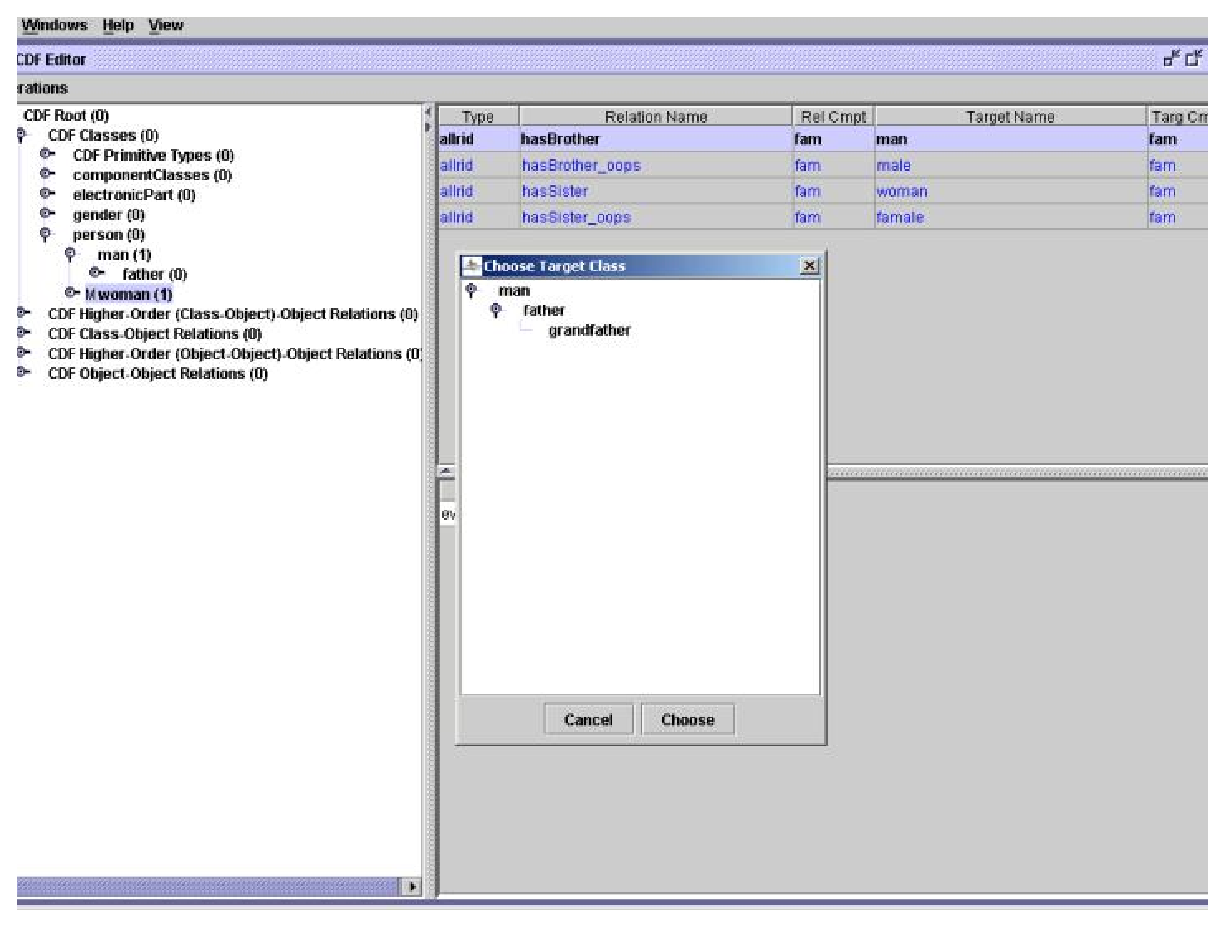
\epsfig{file=Figures/chooseFromTerms.eps,width=\textwidth}}
\caption{An example of {\tt chooseFromTerms/6} based on a term set of type {\tt XJTree}.}
\end{figure}
%-------------------------

%-------------------------------------------------------------------------------------------
\xjitem{xjConfirmUser(+ParWin, +Title, +Message)}{xjConfirmUser/3}
%
Creates a window \footnote{A \jclass{JOptionPane} of type
{\tt Confirm Dialog}.} allowing a user to confirm or cancel an
operation.  An example is shown in Figure~\ref{fig:xjConfirmUser}.

%-------------------------
\begin{figure}[htbp] \label{fig:xjConfirmUser}
\centering {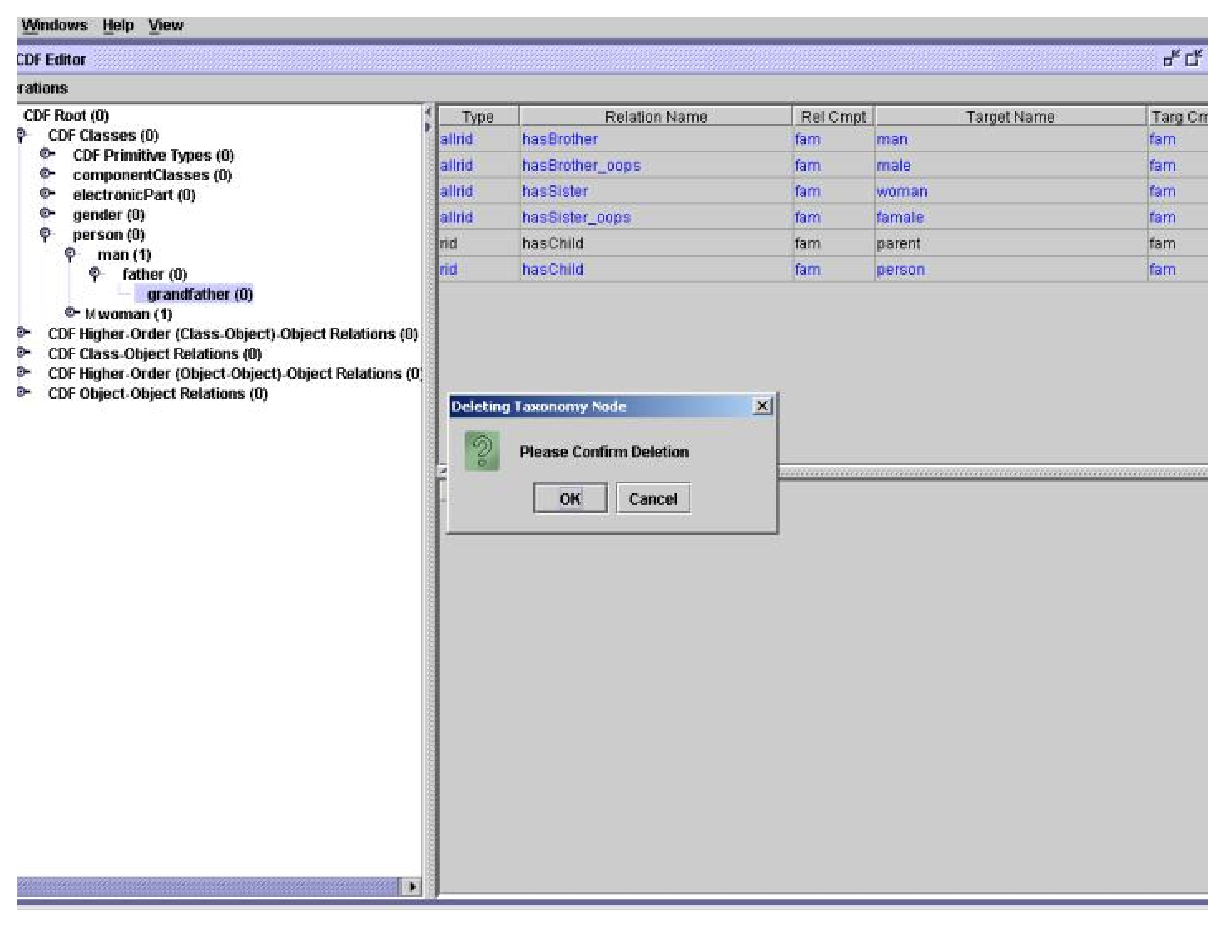
\epsfig{file=Figures/xjConfirmUser.eps,width=\textwidth}}
\caption{An example of xjConfirmUser}
\end{figure}
%-------------------------

%-------------------------------------------------------------------------------------------
%\xjrptitem{xjAskUser(+ParWin,+Question,?DefaultAnswer,-Answer)}{xjAskUser/5}
%
\xjitem{xjAskUser(+ParWin,+Title,+Question,?DefaultAnswer,-Answer)}
	{xjAskUser/5}
%
Creates a window \footnote{A \jclass{JOptionPane} of type {\tt Input
Dialog}.} allowing a user to input data and confirm or cancel that
data once it is input.
%-------------------------------------------------------------------------------------------

\xjitem{xjReportError(+ParWin,+Title,+Message)}{xjReportError/3}
Creates a window \footnote{A \jclass{JOptionPane} of type {\tt
Error Message Dialog} with an error icon.} informing a user of an error
condition specified by {\tt Message}.

\xjitem{xjNotifyUser(+ParWin,+Title,+Message)}{xjNotifyUser/3}
Creates a window \footnote{A \jclass{JOptionPane} of type {\tt
Inform Message Dialog} with a  icon.} notifying the user of an event
or condition specified by {\tt Message}.

%-------------------------------------------------------------------------------------------
%\xjitem{xjAskNumber(+ParWin,+Question,+Title,?InitialValue,+Type,-num(Result))} {xjAskNumber/5}
%
%Produces a modal dialog window  asking the user for a number.  Type can be
%the atom float or the atom Integer.

%-------------------------------------------------------------------------------------------

% Just a generic message.
%\xjitem{xjShowAboutDialog(+ParWin, +Title, +Message, +IconLocation)}
%{xjShowAboutDialog/4}
%Displays generic about dialog. 

%-------------------------------------------------------------------------------------------

% TLS ParWin in different place in the code.
\xjitem{xjShowOptionDialog(+ParWin,+Title,+Message,+ButtonList,-ButtonChosen)} {xjShowAboutDialog/5}
%
Display a modal dialog window \footnote{A \jclass{JOptionPane} of type
{\tt Question Message Dialog}.} with a question message and a set of
buttons to click on to answer that message.  An example is shown in
Figure~\ref{fig:xjShowOptionDialog}.

%-------------------------
\begin{figure}[htbp] \label{fig:xjShowOptionDialog}
\centering {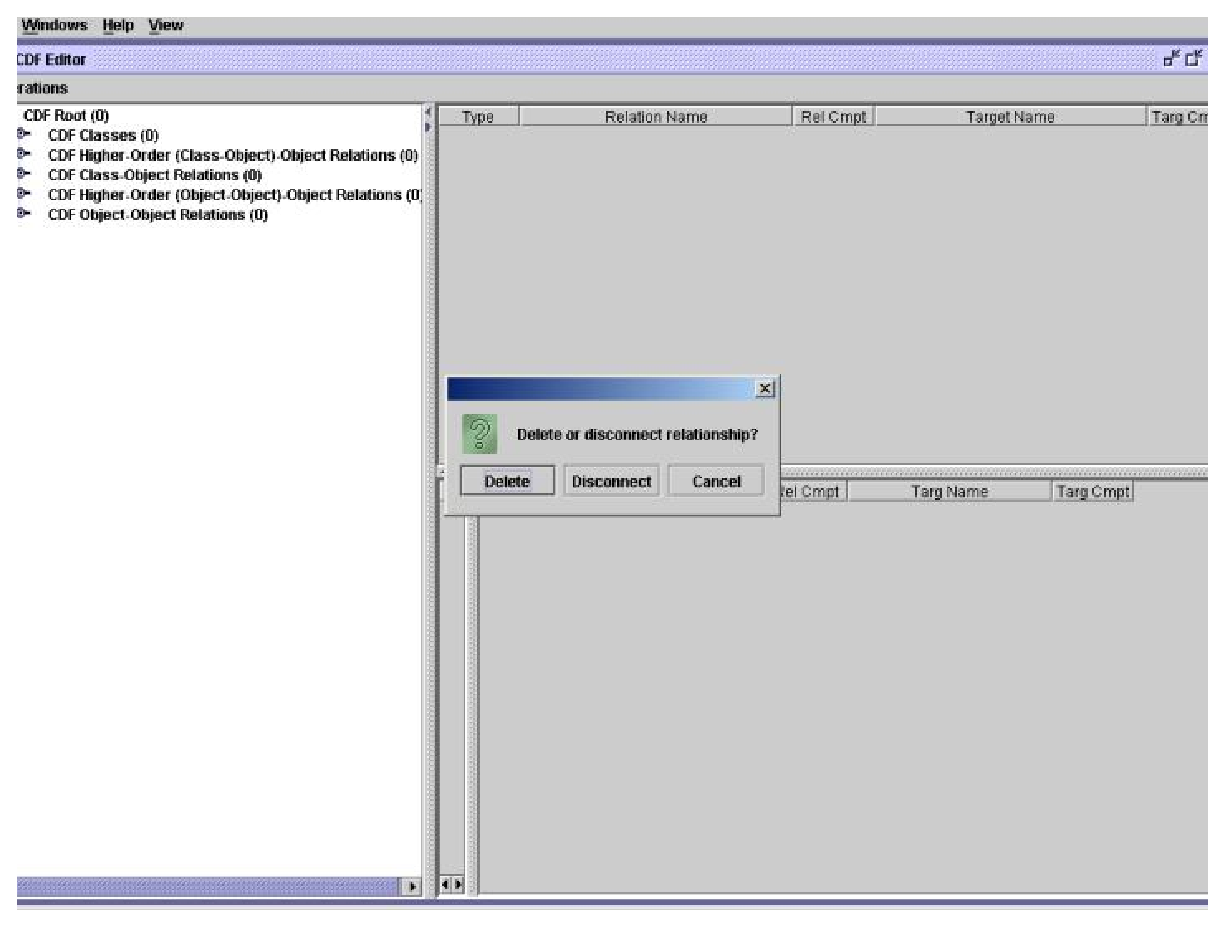
\epsfig{file=Figures/xjShowOptionDialog.eps,width=\textwidth}}
\caption{An example of xjShowOptionDialog}
\end{figure}
%-------------------------

%-------------------------------------------------------------------------------------------

\xjitem{xjPickFile(+Parent,+StartDir,+ExtensionList,+ApproveText,-File)
	}{xjPickFile/5}	
%
%\xjrptitem{xjPickFile(+StartDir,+ExtensionList,+ApproveText,-File)}{xjPickFile/4}
%
%\xjitem{xjPickFile(+ExtensionList,+ApproveText,-File)}{xjPickFile/3}
%
This predicate displays a Swing file chooser, and fails if the user
cancels the choice.  {\tt StartDir} is an atom signifying the starting
directory for the chooser, {\tt ApproveTest} is an atom , and {\tt
ExtensionList} is a list of atoms containing all file types that
should be shown without dot, e.g.  ['P',java].  {\tt xjPickFile/3}
uses the user home directory as the starting directory. {\tt ???
Parent}.

%--------------
\begin{figure}[htbp] \label{fig:xjPickFile}
\centering {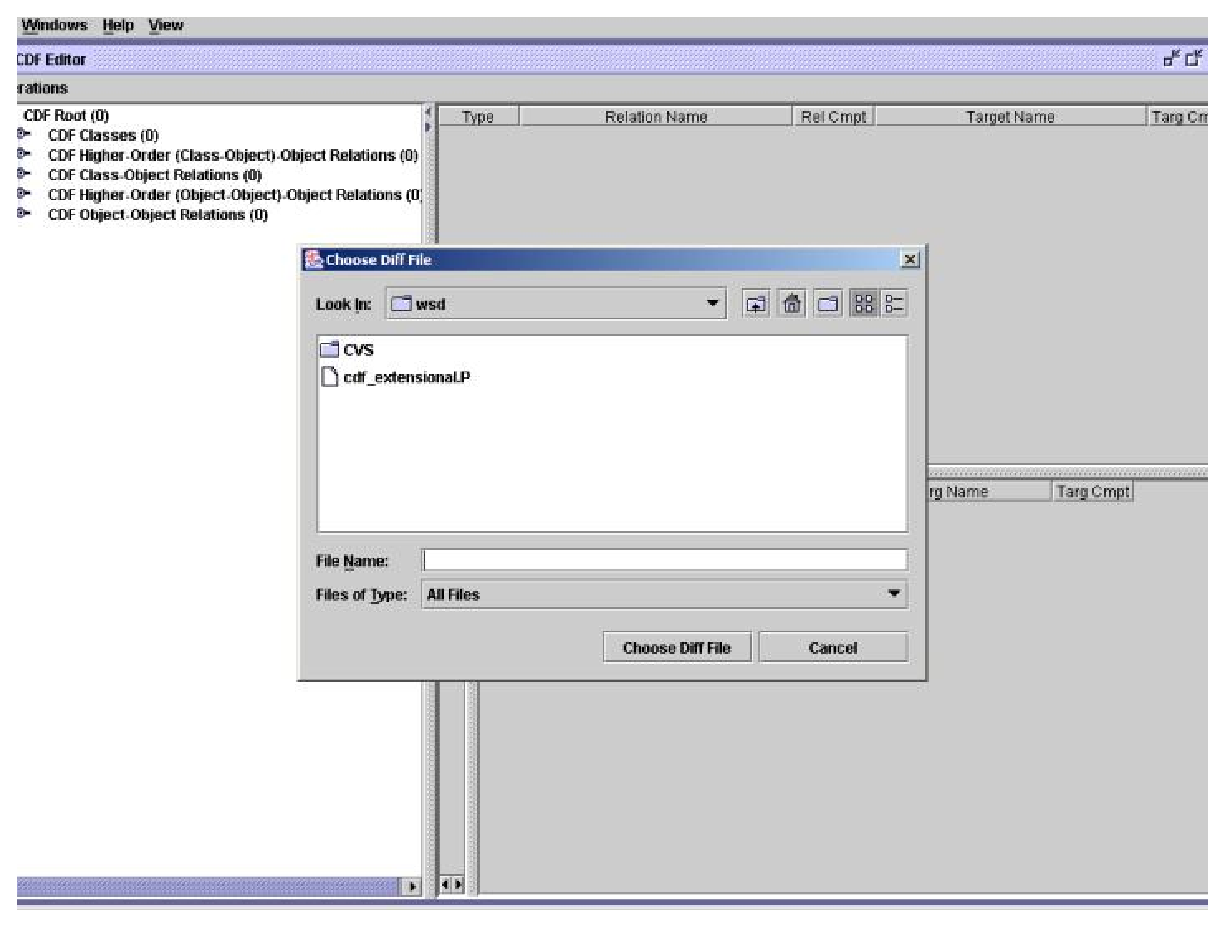
\epsfig{file=Figures/xjPickFile.eps,width=\textwidth}}
\caption{An example of xjPickFile}
\end{figure}
%--------------

\xjitem{xjPickDirectory(+Parent,+StartDir,+ApproveText,-Dir)}{xjPickDirectory/4}
%\xjrptitem{xjPickDirectory(+StartDir,+ApproveText,-File)}{xjPickDirectory/3}
%\xjitem{xjPickDirectory(+ApproveText,-File)}{xjPickDirectory/2}
%
This predicate displays a Swing file chooser, and fails if the user
cancels the choice.  For this predicate, only directories will be
displayed and chosen.  {\tt StartDir} is an atom signifying the
starting directory for the chooser, {\tt ApproveTest} is an atom.
{\tt xjPickDirectory/2} uses the user home directory as the starting
directory. {\tt ???  Parent}.

%-------------------------------------------------------------------------------------------

%\xjitem{xjShowURL(+URL)}{xjShowURL/1}
%Displays URL using system browser.

%\xjitem{xjViewDocument(+Location,+Viewer)}{xjViewDocument/2}
%Allows the use of the system viewer.

%-------------------------------------------------------------------------------------------

% Check out xj_display_errors, editTermGetResult
\end{description}

\subsection{Tree Templates}
	Generic class tree.

\subsection{Toolbar Widgets}
%    createNewMenu('Open',OPMenu),
%    addMenuItem(OPMenu, 'Project ...', open_project_commit),
%    addSubMenu(FileMenu,OPMenu),



\printindex

\end{document}

